% This is the LaTeX source file for the instructions on typesetting PDG
% reviews. It is included with your review source files so you can include
% these instructions into your own review and see some examples.
%
% These same instructions are also provided as a standalone PDF file
% in instructions.pdf.
%
% ---------- Special definitions for PDG review instructions ----------
% The following redefinitions ensure that the example documentation is
% inserted at the correct section level in user reviews:
\let\Isection\section
\let\Isubsection\subsection

\lstdefinestyle{tex}{
	language={[LaTeX]TeX},
	%alsoletter={\\,*,\&},
	basicstyle=\footnotesize\ttfamily,
	texcsstyle=*\ttfamily\color{blue!50!gray},
	keywordstyle=\ttfamily\color{blue!60!gray},
	stringstyle=\ttfamily\color{red!60!gray},
	commentstyle=\ttfamily\color{black!50}, 
	moredelim=**[s][\ttfamily\color{red!60!gray}]{<}{>},
	mathescape,
	%columns=fixed,
    	showtabs=false,
   	keepspaces,
	upquote=true, 
	showstringspaces=false,
	tabsize=4,
	morekeywords={bookcr,bookletcr,webcr,bookalign,bookletalign,webalign,includegraphics,
	setfootnotestyle,captionsetup,rotatebox,multicolumn, multirow, multispan, makecell, iswebbook,balancedlastpagefalse,blankendpagetrue,crossref,tag,xspace},
	breakatwhitespace,
	%literate={>}{}{0},
}
\lstset{style=tex}
\lstnewenvironment{verbtex}{}{}
\newcommand{\invt}[1]{\lstinline!#1!}

%TOC depth
\setcounter{tocdepth}{4}
\setlength{\cftsecnumwidth}{6em} 
\setlength{\cftsubsecnumwidth}{6em} 
\tableofcontents
\setlength{\parskip}{5pt} 
% ---------- End of special definitions for PDG review instructions ----------


\Isection{Typesetting PDG reviews}
These instructions contain documentation and examples for typesetting PDG reviews using the PDG \LaTeX \ class.

They are initially included in the template source files for your own review as an example.
Once you begin writing your review, you should comment out the \lstinline!% This is the LaTeX source file for the instructions on typesetting PDG
% reviews. It is included with your review source files so you can include
% these instructions into your own review and see some examples.
%
% These same instructions are also provided as a standalone PDF file
% in instructions.pdf.
%
% ---------- Special definitions for PDG review instructions ----------
% The following redefinitions ensure that the example documentation is
% inserted at the correct section level in user reviews:
\let\Isection\section
\let\Isubsection\subsection

\lstdefinestyle{tex}{
	language={[LaTeX]TeX},
	%alsoletter={\\,*,\&},
	basicstyle=\footnotesize\ttfamily,
	texcsstyle=*\ttfamily\color{blue!50!gray},
	keywordstyle=\ttfamily\color{blue!60!gray},
	stringstyle=\ttfamily\color{red!60!gray},
	commentstyle=\ttfamily\color{black!50}, 
	moredelim=**[s][\ttfamily\color{red!60!gray}]{<}{>},
	mathescape,
	%columns=fixed,
    	showtabs=false,
   	keepspaces,
	upquote=true, 
	showstringspaces=false,
	tabsize=4,
	morekeywords={bookcr,bookletcr,webcr,bookalign,bookletalign,webalign,includegraphics,
	setfootnotestyle,captionsetup,rotatebox,multicolumn, multirow, multispan, makecell, iswebbook,balancedlastpagefalse,blankendpagetrue,crossref,tag,xspace},
	breakatwhitespace,
	%literate={>}{}{0},
}
\lstset{style=tex}
\lstnewenvironment{verbtex}{}{}
\newcommand{\invt}[1]{\lstinline!#1!}

%TOC depth
\setcounter{tocdepth}{4}
\setlength{\cftsecnumwidth}{6em} 
\setlength{\cftsubsecnumwidth}{6em} 
\tableofcontents
\setlength{\parskip}{5pt} 
% ---------- End of special definitions for PDG review instructions ----------


\Isection{Typesetting PDG reviews}
These instructions contain documentation and examples for typesetting PDG reviews using the PDG \LaTeX \ class.

They are initially included in the template source files for your own review as an example.
Once you begin writing your review, you should comment out the \lstinline!% This is the LaTeX source file for the instructions on typesetting PDG
% reviews. It is included with your review source files so you can include
% these instructions into your own review and see some examples.
%
% These same instructions are also provided as a standalone PDF file
% in instructions.pdf.
%
% ---------- Special definitions for PDG review instructions ----------
% The following redefinitions ensure that the example documentation is
% inserted at the correct section level in user reviews:
\let\Isection\section
\let\Isubsection\subsection

\lstdefinestyle{tex}{
	language={[LaTeX]TeX},
	%alsoletter={\\,*,\&},
	basicstyle=\footnotesize\ttfamily,
	texcsstyle=*\ttfamily\color{blue!50!gray},
	keywordstyle=\ttfamily\color{blue!60!gray},
	stringstyle=\ttfamily\color{red!60!gray},
	commentstyle=\ttfamily\color{black!50}, 
	moredelim=**[s][\ttfamily\color{red!60!gray}]{<}{>},
	mathescape,
	%columns=fixed,
    	showtabs=false,
   	keepspaces,
	upquote=true, 
	showstringspaces=false,
	tabsize=4,
	morekeywords={bookcr,bookletcr,webcr,bookalign,bookletalign,webalign,includegraphics,
	setfootnotestyle,captionsetup,rotatebox,multicolumn, multirow, multispan, makecell, iswebbook,balancedlastpagefalse,blankendpagetrue,crossref,tag,xspace},
	breakatwhitespace,
	%literate={>}{}{0},
}
\lstset{style=tex}
\lstnewenvironment{verbtex}{}{}
\newcommand{\invt}[1]{\lstinline!#1!}

%TOC depth
\setcounter{tocdepth}{4}
\setlength{\cftsecnumwidth}{6em} 
\setlength{\cftsubsecnumwidth}{6em} 
\tableofcontents
\setlength{\parskip}{5pt} 
% ---------- End of special definitions for PDG review instructions ----------


\Isection{Typesetting PDG reviews}
These instructions contain documentation and examples for typesetting PDG reviews using the PDG \LaTeX \ class.

They are initially included in the template source files for your own review as an example.
Once you begin writing your review, you should comment out the \lstinline!% This is the LaTeX source file for the instructions on typesetting PDG
% reviews. It is included with your review source files so you can include
% these instructions into your own review and see some examples.
%
% These same instructions are also provided as a standalone PDF file
% in instructions.pdf.
%
% ---------- Special definitions for PDG review instructions ----------
% The following redefinitions ensure that the example documentation is
% inserted at the correct section level in user reviews:
\let\Isection\section
\let\Isubsection\subsection

\lstdefinestyle{tex}{
	language={[LaTeX]TeX},
	%alsoletter={\\,*,\&},
	basicstyle=\footnotesize\ttfamily,
	texcsstyle=*\ttfamily\color{blue!50!gray},
	keywordstyle=\ttfamily\color{blue!60!gray},
	stringstyle=\ttfamily\color{red!60!gray},
	commentstyle=\ttfamily\color{black!50}, 
	moredelim=**[s][\ttfamily\color{red!60!gray}]{<}{>},
	mathescape,
	%columns=fixed,
    	showtabs=false,
   	keepspaces,
	upquote=true, 
	showstringspaces=false,
	tabsize=4,
	morekeywords={bookcr,bookletcr,webcr,bookalign,bookletalign,webalign,includegraphics,
	setfootnotestyle,captionsetup,rotatebox,multicolumn, multirow, multispan, makecell, iswebbook,balancedlastpagefalse,blankendpagetrue,crossref,tag,xspace},
	breakatwhitespace,
	%literate={>}{}{0},
}
\lstset{style=tex}
\lstnewenvironment{verbtex}{}{}
\newcommand{\invt}[1]{\lstinline!#1!}

%TOC depth
\setcounter{tocdepth}{4}
\setlength{\cftsecnumwidth}{6em} 
\setlength{\cftsubsecnumwidth}{6em} 
\tableofcontents
\setlength{\parskip}{5pt} 
% ---------- End of special definitions for PDG review instructions ----------


\Isection{Typesetting PDG reviews}
These instructions contain documentation and examples for typesetting PDG reviews using the PDG \LaTeX \ class.

They are initially included in the template source files for your own review as an example.
Once you begin writing your review, you should comment out the \lstinline!\input{examples.tex}! line that includes these instructions in the main source file of your review, \invt{databases-main.tex}.

This documentation focuses mostly on the specialized functionality of the PDG \LaTeX \ class: %There are many resources that provide more general guidance for typesetting in \LaTeX.
For further support, or any \LaTeX-related questions, we invite authors to contact
\vspace{-0.2cm}
\begin{center}
\scalebox{1.5}{
	\invt{latexsupport@pdg.lbl.gov}
}
\end{center}

\Isubsection{File structure}
The source files for a PDG review are kept in separate directories within a SVN repository. 
Some files in each directory are auto-generated, while others are designed to be edited by review authors. 
\textbf{Do not edit auto-generated files, as any edits to these files will be overwritten periodically.}

Each review is assigned a unique name ("basename") that is used to label the relevant review files and will be referred to as \invt{BASENAME} in the following. For example, the QCD review is assigned basename \invt{qcd}. Therefore \invt{BASENAME-main.tex} in this documentation refers to file \invt{qcd-main.tex} for the QCD review.

Your review is assigned basename \invt{databases}.

The basename is further used to label cross-references to the review (see Sec.~\ref{sec:labels}) and specialized citations (see Sec.~\ref{sec:cites}). 
The file structure of a typical review is as follows:
\begin{itemize}
\item \invt{BASENAME-main.tex} --- contains the text of your review. 
\item \invt{BASENAME-booklet.tex} --- contains the text of the booklet version of your review (if there is one)
\item \invt{BASENAME-preamble.tex} --- contains review-specific definitions or inclusion of packages, that need to go into the document's preamble
\item \invt{BASENAME.bib} --- BibTeX bibliography entries (see Sec~\ref{sec:cites})
\item \invt{/figures} --- directory containing all figures
\item Auxiliary files (\invt{.aux}, \invt{.out}, \invt{.log}) --- these are generated by the \LaTeX compiler
\item Other \invt{.tex} files --- may be added and included in \invt{BASENAME-main.tex} or \invt{BASENAME-booklet.tex} with the \lstinline{\input} command.
\item \textbf{[auto-generated]} \invt{BASENAME.tex} --- compilation file for the review
\item \textbf{[auto-generated]} \invt{Makefile} --- Makefile to compile the review automatically (see Sec.~\ref{sec:make})
\item \textbf{[auto-generated]} \invt{pdg.cls} --- PDG \LaTeX \ class file
\item \textbf{[auto-generated]} \invt{pdg.bst} --- BibTeX PDG style file
\item \textbf{[auto-generated]} \invt{pdg-xr-hyper.sty} --- helper BibTeX style file
\item \textbf{[auto-generated]} \invt{pdgdefs.tex} --- PDG standard symbols and macros
\item \textbf{[auto-generated]} \invt{examples.tex} --- This file
\end{itemize}

\begin{center}
~\\
%!%\vspace{-12pt}
%!%In your review, the basename is databases.
\end{center}
To identify the  \invt{BASENAME} of yours or another review, you may also login into the 
\href{https://pdgworkspace.lbl.gov/Reviews.action}{PDG Workspace} (click to be redirected). 
Under \emph{Reviews} select from the drop-down menu \emph{All reviews}. 
Click on the title of the review you are interested in, and then select the \emph{Technical details} tab. 
The \invt{BASENAME} is the first entry.

\Isubsection{Multiversion typesetting}
The PDG \LaTeX \ class has functionality to typeset in four different versions or styles: draft, web, book and booklet. 
(The draft and web versions are referred to below jointly as `web', since they are broadly similar). 
See Table~\ref{examples:tab:styles} for a broad summary.

\begin{pdgxtable}[place=h,bookscale = 0.9,bookbbscale=2]
	\caption{Styles for the different typesetting versions}
	\label{examples:tab:styles}
	\begin{pdgxtabular}{ccccc}
		Version 		& Columns  & Font size 	& Helper Tags\footnote{
			Tags for each equation, table, figure, and bibliography entry are displayed in margin or interspaced} & Line numbers\\
		\hline
		\invt{draft} 	& 1		   & 11pt		& Yes & Yes \\
		\invt{web} 		& 1		   & 11pt		& No  & No\\
		\invt{book} 	& 2		   & 8pt		& No  & No\\
		\invt{booklet} 	& 1		   & 8pt		& No & No \\
	\end{pdgxtabular}
\end{pdgxtable}

Specialized macros may also have version-specific implementations. 
These follow the naming convention \invt{<version><macroname>}, where \invt{<version>} may take values of \invt{book}, \invt{booklet} and \invt{web}.
See for example, Sec.~\ref{sec:align}.
Specialized option keys follow the same convention. See e.g. Sec.~\ref{sec:ginkeys}.


\Isubsection{Makefile}
\label{sec:make}
We recommend to compile the review using \invt{make} on the command line. The usage is as follows:
\begin{itemize}
	\item \invt{make} --- compiles in draft mode.
	\item \invt{make  <version>} --- compiles in \invt{<version>} mode. For example \invt{make web}.
	\item \invt{make bib} --- compiles only the BibTeX files.
	\item \invt{make clean} --- cleans out all auxiliary files.
	\item \invt{make cleanall} --- cleans out the compiled pdf and all auxiliary files.
	\item \invt{make prod} --- cleans all auxiliary files, then compiles the web version.
	\item {\footnotesize{\texttt{make crossref}}} --- compiles required cross-referencing files (advanced: requires checkout of the other reviews to be cross-referenced).
\end{itemize}



\Isection{Style guides}
\Isubsection{Particle symbols}
Particle symbols are italic (or slanted) characters: \en, \pbar, \Lb, \pizero, \Klong, \Dstar. 
Charge is indicated by a superscript: $B^{-}$, $\Delta^{++}$. 
Charge is not normally indicated for $p$, $n$, or the quarks, and is optional for neutral isosinglets: $\eta$ or $\eta^{0}$. 
Antiparticles and particles are distinguished by charge for
charged leptons and mesons: $\tau^{+}$, $\kaon^{-}$ 
Otherwise, distinct antiparticles are indicated by a bar (overline): $\nbar_{\mu}$, \tbar, \pbar, \Kzerobar.

\Isubsection{Macros and shortcuts}
The \invt{pdgdefs.tex} file implements a series of useful macros for particle symbols, units and other common notation. 
All definitions are terminated with  \lstinline!\string\xspace!, so you can simply write ``\lstinline!\ttbar production!'' to typeset inline ``\ttbar production''.
The entire list of macros is provided in Sec.~\ref{sec:macros}.

Most Monte Carlo generators have a macro with a suffix 'V' that allows you to include the version. E.g. \lstinline!\PYTHIAV{8.1}! produces \PYTHIAV{8.1}.
In case you need to define other symbols, please add them to the \invt{BASENAME-preamble.tex} file.

\Isubsection{Column switching}

The web version is typeset as single column, singleside 11pt style, the book as 8pt double column, double sided.

In all versions of the review, switching between single and double column mode can be done \emph{in situ} with \lstinline{\onecolumn} or \lstinline{\twocolumn}
respectively. For example

\medskip
\ifrppbook
	\onecolumn
\else
	\twocolumn
\fi
{\footnotesize{Lorem ipsum dolor sit amet, consectetur adipiscing elit. Duis congue lectus at lectus tristique porta. Vivamus scelerisque porta massa, laoreet pulvinar dolor blandit vitae. Nam rhoncus id risus in tincidunt. Maecenas ultrices, arcu id gravida tempor, urna libero sodales nunc, quis dapibus ipsum quam eget est. Quisque eget convallis odio, at pellentesque quam. Mauris pretium eu metus ac imperdiet. Class aptent taciti sociosqu ad litora torquent per conubia nostra, per inceptos himenaeos. Nulla quis tincidunt libero. Aliquam posuere at quam quis posuere. Etiam turpis nulla, faucibus eget massa sagittis, porttitor sagittis elit. Proin a lorem eleifend, rhoncus orci quis, mattis metus. Donec sit amet lobortis lacus. Quisque magna augue, elementum nec ipsum non, feugiat ultricies urna. Sed tincidunt nisl vestibulum leo finibus, vitae sollicitudin sapien bibendum. Duis maximus ipsum nec urna lobortis, sed scelerisque nulla facilisis. Sed id finibus libero. }}
\ifrppbook
	\twocolumn
\else
	\onecolumn
\fi
\medskip

\Isection{Equations}
Equations may be typeset using the \invt{equation}, \invt{array}, \invt{multline}, and \invt{gather} etc environments provided by \invt{amsmath} package. 
We do not recommend using \invt{eqnarray}. As a trivial example
\begin{verbtex}
\begin{equation}
\label{BASENAME:eq:equation}
	N_{exp} = \sigma_{exp} \times \int L(t) dt
\end{equation}
\end{verbtex}
which produces
\begin{equation}
	N_{exp} = \sigma_{exp} \times \int L(t) dt
\end{equation}


To tag a set of equations with a common numbering and label, please use the \invt{subequation} environment, together with \invt{align}.
As an example:
\begin{verbtex}
\begin{subequations}
	\label{BASENAME:eq:equation1}
	\begin{align}
		A + B = C\\
		D= \frac{E}{F}  
	\end{align}
\end{subequations}
\end{verbtex}
which produces
\begin{subequations}
\begin{align}
	A + B = C\\
	D= \frac{E}{F}  
\end{align}
\end{subequations}


\Isubsection{Wide equations: \invt{pdgstrip}}
Some wide equations are not easily amenable to display in the PDG book double column format. 
Similar to the ReVTeX \invt{widetext} environment, the PDG style provides a \invt{pdgstrip} environment, that may wrap any other equation (or align, array etc) environment. 
The \invt{pdgstrip} environment is not a float, and will respect absolute placement in the typesetting stream. 
For example:
\begin{verbtex}
	\begin{pdgstrip}
		\begin{equation} % or any other display environment
		...

		\end{equation}
	\end{pdgstrip}
\end{verbtex}
In the web and booklet versions, this environment performs no operation on the wrapped environment. 
In the book version, the equation is preserved as a single `strip' across both columns, with column-wide rules to guide the reader's eye. 
The column-wide rules may be disabled -- e.g if the strip environment falls at the top or bottom of a page --  by passing the option \invt{plain} to the \invt{pdgstrip} environment. I.e. 
\lstinline!\begin{pdgstrip}[plain]!.

In principle, the pdgstrip envirornment may also wrap a floating environment such as a figure. 
In the book version, this will disable the ability of the figure to float, and fix it to a desired location.

\Isubsection{Alignment}
\label{sec:align}
Within \invt{align} environments or any other environment that uses the special \invt{&} and \invt{\\\\} (or \lstinline{\cr}) control characters for alignment, one may use
use version specific \lstinline!\bookalign!, \lstinline!\webalign!, \lstinline!\bookletalign! and \lstinline!\bookcr!, \lstinline!\webcr!, \lstinline!\bookletcr! macros.

The \lstinline!\<version>align! macros insert a `\invt{&}' control character only in the \invt{<version>} of the review. 
The \lstinline!\<version>cr! macro similarly inserts a carriage return `\invt{\\\\}' only in the \invt{<version>} of the review, 
but takes two additional arguments that are placed before and after the carriage return, respectively. For instance,
\lstinline!\bookcr{\nonumber}{[10pt]}! inserts \lstinline!\nonumber\\[10pt]!.  An example usage is
\begin{verbtex}
\begin{align}
	{\cal A}_f 
	\bookalign = \frac{\Gamma(\bar{B}^0(t) \to f) - \Gamma(B^0(t) \to f)}
		{\Gamma(\bar{B}^0(t) \to f) + \Gamma(B^0(t) \to f)} \bookcr{\,,\nonumber}{}
	\bookalign = S_f \sin(\Delta m_d\, t) - C_f \cos(\Delta m_d\, t) \,.
\end{align}
\end{verbtex}
This produces in the web version
\ifrppbook
\onecolumn
	\begin{align}
		{\cal A}_f  = \frac{ \Gamma(\bar{B}^0(t) \to f) - \Gamma(B^0(t) \to  f) }
			{ \Gamma(\bar{B}^0(t) \to f) + \Gamma(B^0(t) \to  f) } 
			= S_f \sin(\Delta m_d\, t) - C_f \cos(\Delta m_d\, t) \,,
	\end{align}
\twocolumn
\else
	\begin{align}
		{\cal A}_f 
		\bookalign = \frac{ \Gamma(\bar{B}^0(t) \to f) - \Gamma(B^0(t) \to  f) }
			{ \Gamma(\bar{B}^0(t) \to f) + \Gamma(B^0(t) \to  f) } \bookcr{\,,\nonumber}{}
		\bookalign = S_f \sin(\Delta m_d\, t) - C_f \cos(\Delta m_d\, t) \,,
	\end{align}
\fi	
and in the two column book version
\addtocounter{equation}{-1}
\ifrppweb
	\twocolumn
	\begin{align}
		{\cal A}_f 
		& = \frac{ \Gamma(\bar{B}^0(t) \to f) - \Gamma(B^0(t) \to  f) }
			{ \Gamma(\bar{B}^0(t) \to f) + \Gamma(B^0(t) \to  f) } \,,\nonumber\\
		& = S_f \sin(\Delta m_d\, t) - C_f \cos(\Delta m_d\, t) \,,
	\end{align}
	\onecolumn
\else
	\begin{align}
		{\cal A}_f 
		\bookalign = \frac{ \Gamma(\bar{B}^0(t) \to f) - \Gamma(B^0(t) \to  f) }
			{ \Gamma(\bar{B}^0(t) \to f) + \Gamma(B^0(t) \to  f) } \bookcr{\,,\nonumber}{}
		\bookalign = S_f \sin(\Delta m_d\, t) - C_f \cos(\Delta m_d\, t) \,,
	\end{align}
\fi

\Isection{Figures}

\Isubsection{Figure requirements}
Permitted figure formats (for pdflatex) are pdf, png and jpg, in order of preferred format. 
In addition, please note:
\begin{itemize}
	\item Submissions should be be provided with a minimum resolution of 150DPI. However, 300DPI or greater is preferred.
	\item Our preference for the submission color palette is CMYK, but RGB is acceptable.
	\item Visible line (stroke) weight must be no less than $0.5$px, preferably at least $1$px.
	\item Submissions should be provided with fonts embedded, if possible.
	\item In print, colors are often not as vibrant or saturated as they appear on screen. Therefore, overlapping areas of color should be high contrast for visual clarity: 
	e.g. do not place magenta over blue, or light blue over a light green.	
\end{itemize}
If you are unsure your figure is of sufficient resolution or quality, please contact \invt{latexsupport@pdg.lbl.gov} for advice.

Encapsulated postscript or postscript figures may also be used, but they require conversion to pdf. 
Depending on your \LaTeX \ engine settings, running \invt{pdflatex} may automatically convert eps or ps files. 
If not, the conversion can be done manually with various programs, such as ImageMagick, or \invt{epstopdf} and \invt{pstopdf}.

\textbf{Note:} Make sure that the figure file is added into the subdirectory \invt{figures}, and that it is commited to svn or provided with your text.

\Isubsection{\invt{pdgxfigure} environment}
The multipurpose figure environment \invt{pdgxfigure} is now available, as an alternative to the various \invt{pdgfigure} and related commands.
These operate similarly to the standard \invt{figure} environments: \invt{(pdgx)figure} creates a floating environment.

The \lstinline!\caption! and \lstinline!\label! commands may be used as in the usual \invt{figure} environment. 
\textbf{Note: A figure caption should be placed below the figure.}
In addition, \invt{pdgxfigure} takes an array of additional option keys that implement features and formatting of the prior PDG figure commands.
These include keys that control placement, multicolumn spanning, and version-specific widths. 
The generic usage is
\begin{verbtex}
\begin{pdgxfigure}[<option keys>]
	\caption{This is a PDG figure}
	\label{examples:fig:label}
	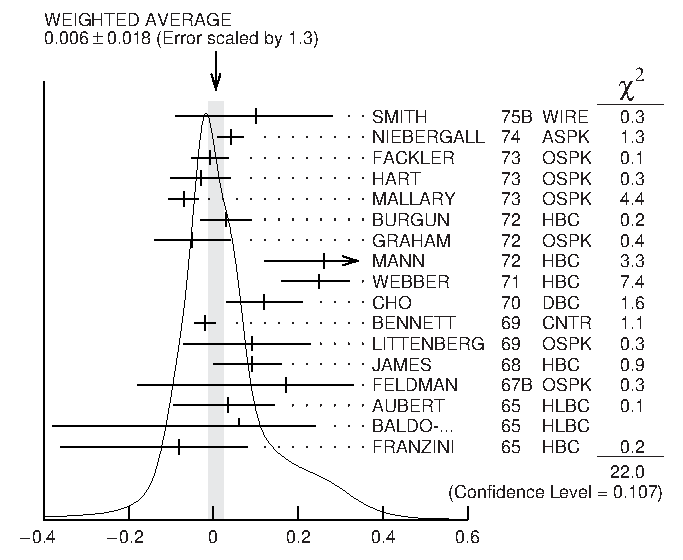
\includegraphics{filename} %multiple includegraphics may be used, 
	% with usual \hfill and \\ newline structures. 
\end{pdgxfigure}
\end{verbtex}

Figures placed in the \invt{figures} directory will be automaticallly found. 
Option keys may also be passed to individual \lstinline{\includegraphics} commands,  
as usual, if separate control is desired of multiple \lstinline{\includegraphics} in the same \invt{pdgxfigure} environment.
I.e. \lstinline!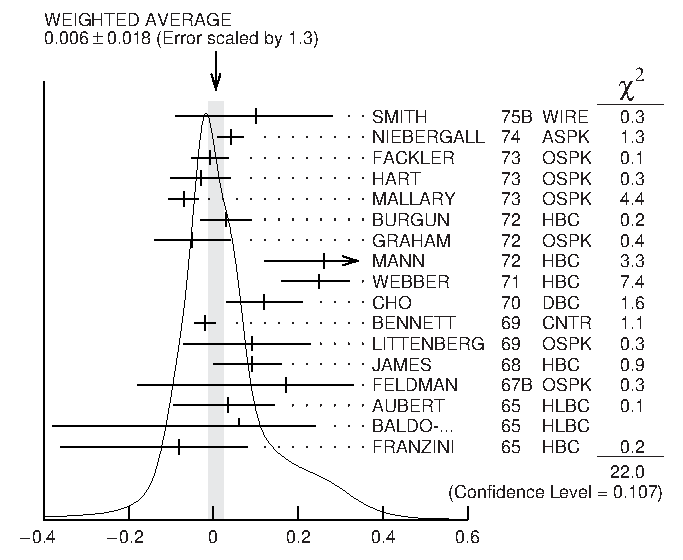
\includegraphics[<option keys>]{filename}!.

\Isubsection{Float scaling and width keys}
\label{sec:ginkeys}
As in the usual implementation of the \invt{graphicx} package, the \lstinline{\includegraphics} command takes optional standard keys \invt{width = ...}, \invt{scale = ...}.
which are used to control the width or scale of the bounding box. 
We use the same key structure to pass options to the \invt{pdgxfigure} environment, as well as to the \invt{pdgxtable} environment (see Sec.~\ref{sec:tables}).

The version specific keys \lstinline!<version>width! and \lstinline!<version>scale! have been added, 
that implement width or scaling choices only in the specific \invt{<version>}.
One may use these keys in concert with the usual \invt{width} and \invt{scale} keys, with the caveat that the order of keys matters: 
Keys are read left to right, and rightwards keys typically override leftwards ones. 
For example, passing the option keys (to either \invt{pdgxfigure} or \invt{pdgxtable}, or \lstinline{\includegraphics})
\begin{verbtex}
	[width=0.8\linewidth, bookwidth=0.9\linewidth]
\end{verbtex}
implements the \invt{width} key setting except in the book version. 
The option \lstinline!bookwidth=0.9\linewidth! followed by
\lstinline!width=0.8\linewidth! would instead implement only the version-general \lstinline!width=0.8\linewidth! setting.

\textbf{Note:} Because of specialization of the \invt{graphicx} key structure in the PDG class,
to use a \invt{scale} or \invt{<version>scale} key in an \lstinline{\includegraphics} command or \invt{pdgxfigure} environment
one must first pass an option key \invt{width=!}. This is not required for  \invt{pdgxtable}.

An additional key \lstinline!<version>bbscale! scales the float bounding box.
For some overwide floats that are larger than the nominal page width---in particular, overwide tables, see Sec.~\ref{sec:tables}---simply 
rescaling down the float does not allow it to be properly aligned on the page.
This key can be increased above $1$ (the default), to provide a sufficiently large bounding box for the float, that may then be scaled down to size with correct alignment.

\Isubsection{Available keys for \invt{pdgxfigure}}
Following is a list of available optional keys for \invt{pdgxfigure}, and default settings if not invoked.
As usual, keys are evaluated left to right. 
The version-general \invt{width} key can be used (and will override any preceeding version-specfic width key).
\begin{itemize}
	\item \invt{place}: Takes any combination of \invt{h}, \invt{t}, \invt{b}, \invt{p} (with optional \invt{\!}) that specifies float placement. Default is \invt{\!ht}.
	\item \invt{wide}: Takes \invt{true} or \invt{false} to specify the figure as full page width in either single or two column mode. Default is \invt{false}.
	\item \invt{width} or \invt{<version>width}: Sets the global or version specific width of the figure bounding box, respectively. Default is 0.75 of the line width (or text width, for wide figures).
	\item \invt{scale} or \invt{<version>scale}: Scales the figure according to float value passed to the key. 
	The option \lstinline{width=!} must be passed to turn off default width behavior and enable scaling keys.
\end{itemize}

\Isubsection{Examples}
The following produces a default-style, shown in Figure~\ref{examples:fig:example}. 
We recommend including the file extension in the \lstinline{\includegraphics} argument, to assist our editorial staff in addressing any figure quality problems.
\begin{verbtex}
\begin{pdgxfigure}[place=t] 
	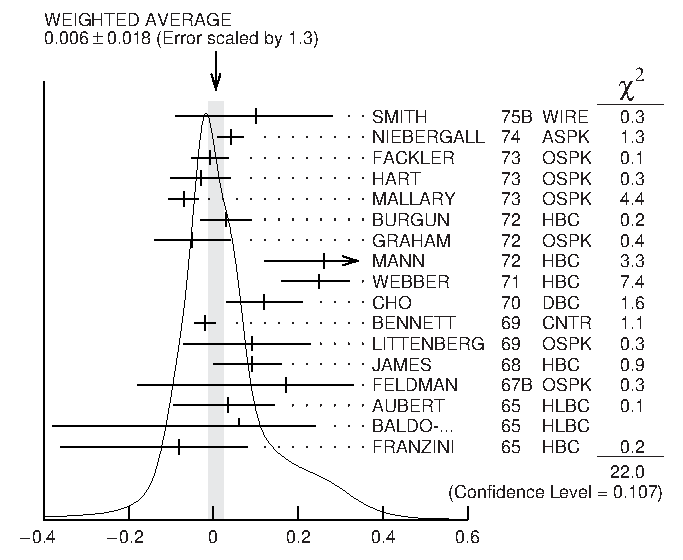
\includegraphics{filename.pdf}
	\caption{Example default figure}
	\label{examples:fig:example}
\end{pdgxfigure}
\end{verbtex}
\begin{pdgxfigure}[place=t]
	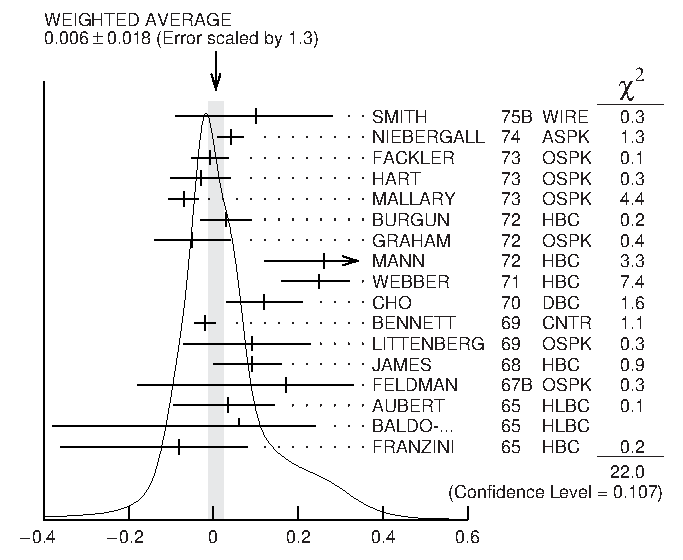
\includegraphics{filename.pdf}
	\caption{Example default figure}
	\label{examples:fig:example}
\end{pdgxfigure}

A double wide figure, shown in Fig.~\ref{examples:fig:example2}:
\begin{verbtex}
\begin{pdgxfigure}[wide=true,place=h, webwidth=0.45\linewidth, 
		bookwidth=0.9\linewidth] 
	%width key applies to all includegraphics instances
	%compiling in different versions will produce different widths
	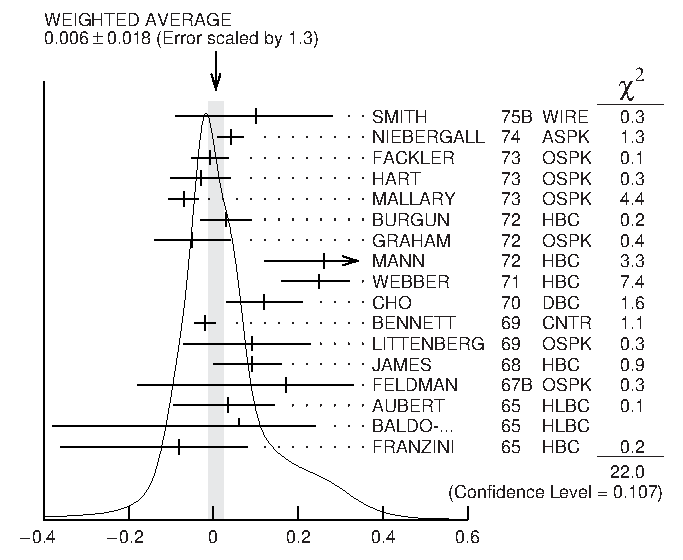
\includegraphics{filename.pdf}\hfill
	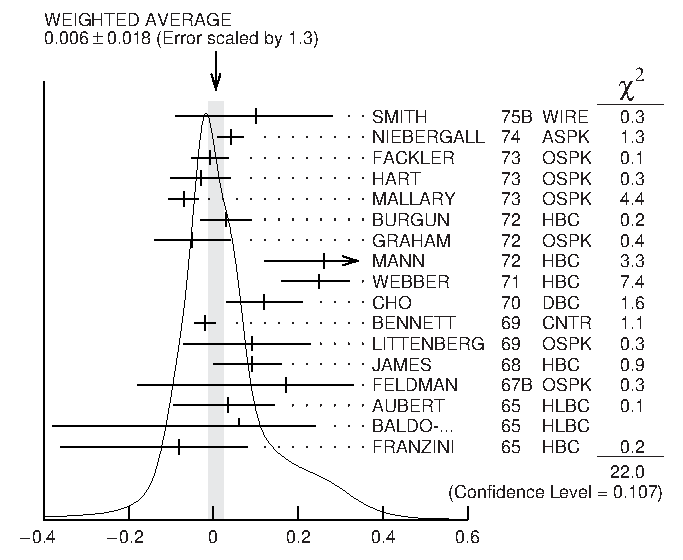
\includegraphics{filename.pdf}
	\caption{Example double wide figure, 
		with different book and web versions}
	\label{examples:fig:example2}
\end{pdgxfigure}
\end{verbtex}
\begin{pdgxfigure}[wide=true,place=h,width=0.45\textwidth] 
	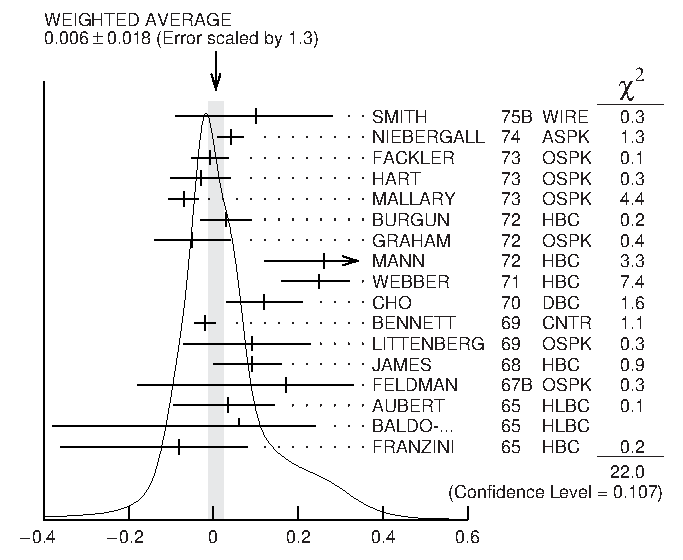
\includegraphics{filename.pdf}\hfill
	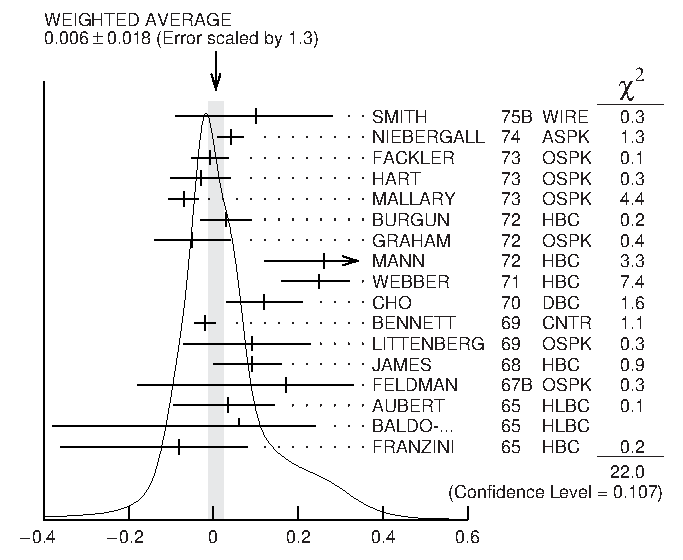
\includegraphics{filename.pdf}
	\caption{Example double wide figure, with different book and web versions}
	\label{examples:fig:example2}
\end{pdgxfigure}

A double wide figure with separate option and scaling keys, shown in Fig.~\ref{examples:fig:example3}:
\begin{verbtex}
\begin{pdgxfigure}[wide=true,place=h,width = 0.3\linewidth] 
	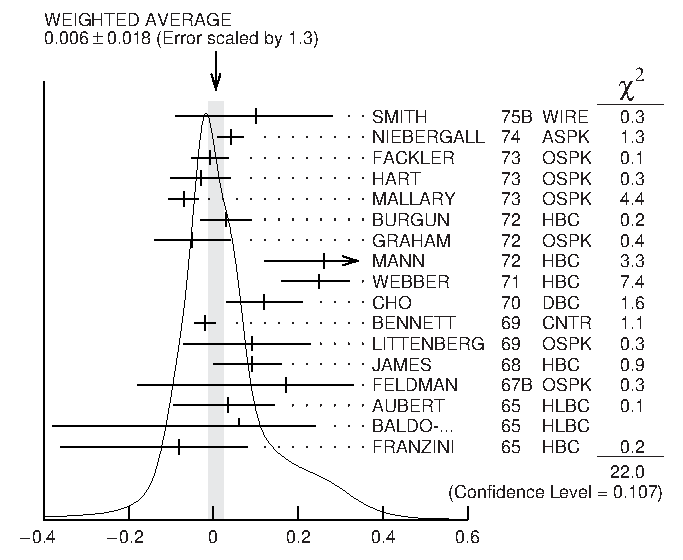
\includegraphics{filename.pdf}\hspace{1cm}
	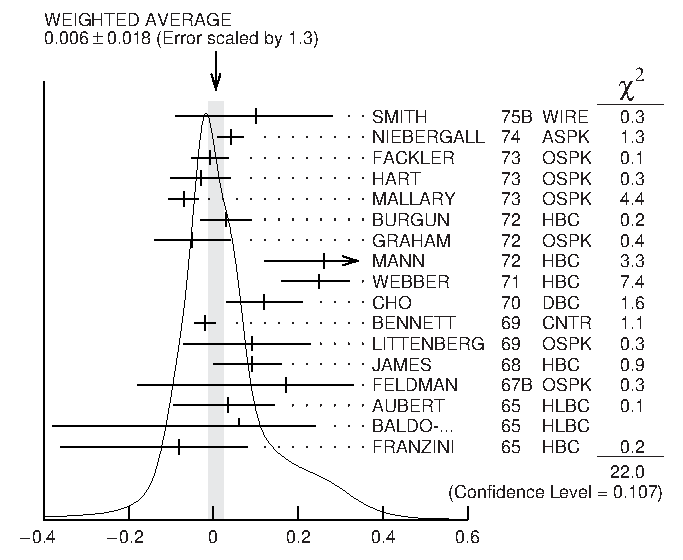
\includegraphics[width = !,scale =0.3,angle = 90]{filename}
	\caption{Example double figure, 
		with separate option and scaling keys, in both book and web versions}
	\label{examples:fig:example3}
\end{pdgxfigure}
\end{verbtex}
\begin{pdgxfigure}[wide=true,place=h,width = 0.3\linewidth] 
	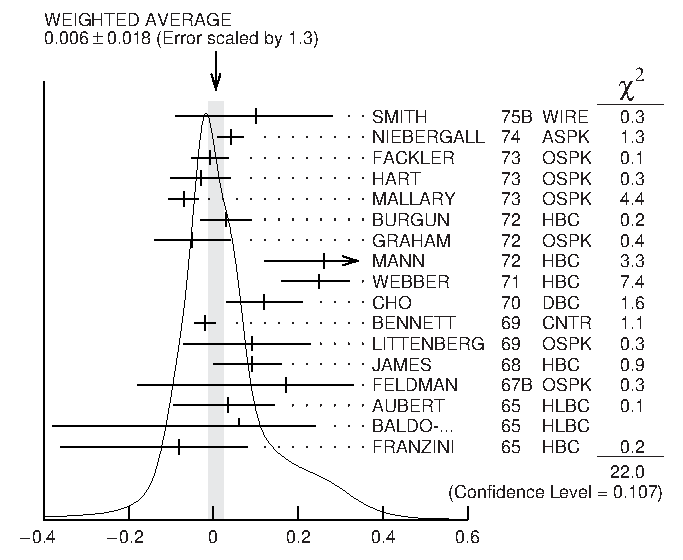
\includegraphics{filename.pdf}\hspace{1cm}
	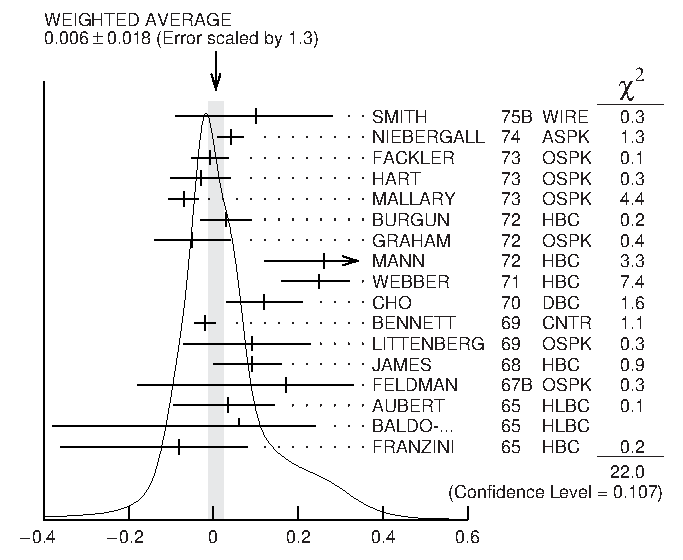
\includegraphics[width = !,scale =0.3,angle = 90]{filename}
	\caption{Example double wide figure, with separate option and scaling keys, in both book and web versions}
	\label{examples:fig:example3}
\end{pdgxfigure}

\Isubsection{\invt{pdgfigure} commands}
To add a figure, one may also use the \lstinline{\pdgfigure} or \lstinline{\pdgwidefigure} commands 
to typeset a single-column figure or double-column wide figure (for the book version), respectively. 
To include two images in one figure one may use \lstinline{\pdgdoublefigure}.
These commands are less powerful than \invt{pdgxfigure}, but automatically incorporate all PDG styles.

The macros \lstinline{\pdgfigure} and \lstinline{\pdgwidefigure} take the following arguments:
\begin{verbtex}
	\pdgfigure{<filename>}
	{<caption>}{<label>}{<placement options>}
	{<other option keys>}
\end{verbtex}
\vspace{-10pt}
while the macro \lstinline{\pdgdoublefigure} takes the following arguments:
\begin{verbtex}
	\pdgdoublefigure{<filename1>}{<filename2>}
	{<caption>}{<label>}{<placement options>}
	{<other option keys>}
\end{verbtex}
Some examples of the \invt{pdgfigure} commands are shown in Figs.~\ref{examples:fig:ideogram1}, \ref{examples:fig:ideogram2} and \ref{examples:fig:ideogram3}, respectively:
\begin{verbtex}
	\pdgfigure{filename.pdf}{Figure with caption and label}
	{examples:fig:ideogram1}{ht!}{}
	
	\pdgdoublefigure{filename.pdf}{filename.pdf}
	{Two figures, with caption and label, reduced in size}
	{examples:fig:ideogram2}{ht!}{width=0.3\textwidth}
	
	\pdgwidefigure{filename.pdf}{Wide figure}
	{examples:fig:ideogram3}{t}{}
\end{verbtex}
\FloatBarrier
\pdgfigure{filename.pdf}{Figure with caption and label}{examples:fig:ideogram1}{ht!}{}
\pdgdoublefigure{filename.pdf}{filename.pdf}{Two figures, with caption and label, reduced in size}{examples:fig:ideogram2}{ht!}{width=0.3\textwidth}
\pdgwidefigure{filename.pdf}{Wide figure}{examples:fig:ideogram3}{t}{}
\FloatBarrier

\Isection{Tables}
\label{sec:tables}
\Isubsection{ \invt{pdgxtable} and \invt{pdgxtabular}}
The PDG class provides multipurpose table and tabular environments, \invt{pdgxtable} and \invt{pdgxtabular}. 
These operate similarly to the standard \invt{table} and \invt{tabular} environments: \invt{(pdgx)table} creates a floating environment, 
while \invt{(pdgx)tabular} creates the actual tabulated display. 

The \lstinline!\caption! and \lstinline!\label! commands may be used as in the usual \invt{table} environment.
\textbf{Note: A table caption should be placed above the table.}
In addition, \invt{pdgxtable} takes a wide array of additional option keys that implement features and formatting of the prior PDG table commands/environments.  
These include keys that control placement, multicolumn spanning, version-specific widths and scaling (see Sec.~\ref{sec:ginkeys}), rotation, stretching, and caption widths.
The generic usage is
\begin{verbtex}
\begin{pdgxtable}[<option keys>]
	\caption{This is a PDG table}
	\label{tab:label}
	\begin{pdgxtabular}{<column settings>} % the usual c, l, r, | etc
		\pdgtableheader{...} %column header & separated entries go here
		%table & separated entries go here
	\end{pdgxtabular}
	%multiple pdgtabular environments are allowed
\end{pdgxtable}
\end{verbtex}

As for the usual \invt{table} environment, one may include multiple \invt{pdgxtabular}s in a single \invt{pdgxtable}.
While the \invt{pdgxtable} environment has default handling for caption widths in wide and regular tables, for both book and web versions, 
absolute control of the caption width can be implmented with a \lstinline{\captionsetup} command inside the \invt{pdgxtable} environment. 
For example \lstinline!\captionsetup{width=\linewidth}! gives a full width caption.

\Isubsection{Available keys for \invt{pdgxtable}}
Following is a list of available optional keys, and default settings if not invoked.
As usual, keys are evaluated left to right. 
While, the version-general \invt{width} key can be used (and will override any preceeding version-specfic width key), 
there is no version-general \invt{scale} key. 
Scaling of the tables is best done with the \invt{<version>scale} keys.

\begin{itemize}
	\item \invt{place}: Takes any combination of \invt{h}, \invt{t}, \invt{b}, \invt{p} (with optional \invt{\!}) that specifies float placement. Default is \invt{\!ht}.
	\item \invt{wide}: Takes \invt{true} or \invt{false} to specify the table as full page width in either single or two column mode. Default is \invt{false}.
	\item \invt{width} or \invt{<version>width}: Sets the version specific maximum width of the table bounding box. 
	Default is the maximum text width implied by the \invt{wide} key setting.
	Width settings exceeding this default are ineffective. Footnotes are scaled, but caption width is not affected.
	\item \invt{<version>scale}: Scales the table according to float value passed to the key. 
	For overwide tables, there is always a value $<1$ at which the table will be properly set to maximum page width.
	Footnotes are scaled, but caption width is not affected. Note the global \invt{scale} is disabled for \invt{pdgxtable}.
	\item \invt{<version>bbscale}: Scales the bounding box of the table. 
	For some overwide tables that are larger than the nominal page width, simply rescaling down the table does not allow the table to be properly aligned on the page.
	This key can be increased above $1$ (the default), to provide a sufficiently large bounding box for the table, that may then be scaled down to size with correct alignment.
	\item \invt{widecaptionscale}: For \invt{wide = true} tables, scales the caption width with respect to the maximum page width. Default is $0.75$.
	\item \invt{narrowcaptionscale}: For \invt{wide = false} or default tables, scales the caption width with respect to the maximum column width. Default is $0.9$.
	\item \invt{rotated}: Takes \invt{left} or \invt{right} to rotate the table, but not the caption, $90^\circ$ anticlockwise or clockwise, respectively. 
	The caption may be rotated independently, as needed with a \lstinline{\rotatebox}.
	\item \invt{sideways}: Takes \invt{true} or \invt{false} to rotate the table, including the caption, $90^\circ$ anticlockwise or clockwise, 
	according to whether the page number is even or odd.
	In a sideways table, other key width and scaling settings are still effective, but scale with respect to the page height. 
\end{itemize}


\Isubsection{Examples}
Some (simple) examples of \invt{pdgxtable} can be found in Table~\ref{examples:tab:styles} and Sec~\ref{sec:macros}.
For example, Tab.~\ref{examples:tab:styles} is typeset as
\begin{verbtex}
\begin{pdgxtable}[place=h,bookscale = 0.9,bookbbscale=2]
	\caption{Styles for the different typesetting versions}
	\label{examples:tab:styles}
	\begin{pdgxtabular}{ccccc}
		Version 		& Columns  & Font size 	& Helper Tags\footnote{
			Tags for each equation, table, figure, and bibliography entry 
			are displayed in margin or interspaced} & Line numbers\\
		\hline
		draft	& 1		   & 11pt		& Yes & Yes \\
		...
	\end{pdgxtabular}
\end{pdgxtable}
\end{verbtex}

Tables~\ref{examples:tab:commu} and~\ref{examples:tab:commp} are typeset as a two \invt{pdgxtabular}s in a single \invt{pdgxtable}, via
\begin{verbtex}
\begin{pdgxtable}[wide=true, place=!ht, webscale = 0.8]
	\caption{Common units}
	\label{examples:tab:commu}
	\begin{pdgxtabular}{lr | lr | lr}
		\showsymbol{\TeV} &  \showsymbol{\syin} & \showsymbol{\barn}   \\
		...
	\end{pdgxtabular}
	\caption{Common particles}
	\label{examples:tab:commp}
	\begin{pdgxtabular}{lr | lr | lr}
   		\showsymbol{\pp} &  \showsymbol{\ee} & \showsymbol{\pizero}   \\
  		...
	\end{pdgxtabular}
\end{pdgxtable}
\end{verbtex}

\Isubsection{Common problems and recommendations}
The \invt{pdgxtabular} environment is capable of handling the usual \lstinline{\multicolumn} and \lstinline{\multirow} objects, 
that allow for more complicated tables with cells spanning multiple rows and/or columns. 
We recommend avoiding use of \lstinline{\multispan}. 
For multiline cells, the \lstinline{\makecell} command from the \invt{makecell} package is recommended.

\Isection{Labels and referencing}
\label{sec:labels}

\Isubsection{Style guide}
As usual, the \lstinline{\label} and \lstinline{\ref} commands (and their derivatives) may be used to reference equations, tables, figures, and so on. 
To permit easy cross-referencing throughout the entire review, we request that you use the following labelling convention: \invt{BASENAME:type:name}
with \invt{type} corresponding to one of the following options
\begin{itemize}
\item {\tt fig} for figures
\item {\tt eq } for equation
\item {\tt tab} for tables
\item {\tt sec} for section, subsection etc..
\item {\tt foot} for footnotes.
\end{itemize}

\Isubsection{Missing references}

In default LaTeX, missing references are typically typeset as ``\textbf{??}''. 
To improve the typesetting experience, the \lstinline{\ref} command has been modified in the PDG class so that missing reference keys are printed out explicitly: 
For instance, a \lstinline!\ref{eqn:name}! that references a missing label called \invt{eqn:name}, will display as \ref{eqn:name}.
Similarly, the \lstinline{\cite} command will explicitly print out missing citation references. E.g. 
a \lstinline!\cite{name:2021ab}! that references a missing label called \invt{name:2021ab}, will display as \cite{name:2021ab}

\Isubsection{Cross-review referencing}
It is occasionally necessary or useful to reference (sub)sections, equations, figures, tables and so on belonging to other reviews or other reviews themselves. 
\textbf{Note:} Please use the \lstinline{\crossref} command for cross-review referencing.

Implementing a cross-reference to another review requires knowledge of its  \invt{BASENAME}:  
You must use the \invt{BASENAME} associated with the target review, not the \invt{BASENAME} of the review you're currently working on. 
To identify the  \invt{BASENAME} of another review, login into the \href{https://pdgworkspace.lbl.gov/Reviews.action}{PDG Workspace} (click to be redirected). 
Under \emph{Reviews} select from the drop-down menu \emph{All reviews}. 
Click on the title of the review you are interested in, and then select the \emph{Technical details} tab. 
The \invt{BASENAME} is the first entry.


If the full \invt{BASENAME:type:name} reference is known, you may include it with the usage \\
\lstinline!\crossref{BASENAME:type:name}!. 
This will typeset in your document as ``\crossref{BASENAME:type:name}'', because your local auxiliary files do not have the reference information of the other review.
PDG editorial staff will implement the cross-reference properly, when your review is prepared for production.

If the \invt{BASENAME:type:name} reference is not known, or the authors of the other review did not label the obect that you wish to reference, 
you may instead provide any descriptive argument to \lstinline{\crossref}. 
For example, \lstinline!\crossref{Equation 34.1.10}!.  
PDG editorial staff will implement the cross-reference properly, when your review and the other review are prepared for production.

\Isubsection{Booklet labeling and referencing}
If your review has a booklet version, it needs to be prepared at the same time as you prepare your full review.
The content to be displayed in the booklet needs to be included in \invt{BASENAME-booklet.tex}. 

The numerical tags for equations, tables, and figures in the booklet version of a review should match the tags in the full version. 
This can be achieved automatically in the booklet version by using a \lstinline!\tag{\ref{BASENAME:type:name}}! construction instead of \lstinline{\label}
to refer to the reference in the full version.
For example, if the full version has a labelled equation
\begin{verbtex}
\begin{equation}
	\label{BASENAME:eq:name}
	...
\end{equation}
\end{verbtex}
then including in \invt{BASENAME-booklet.tex}
\begin{verbtex}
\begin{equation}
	\tag{\ref{BASENAME:eq:name}}
	...
\end{equation}
\end{verbtex}
will automatically label the equation correctly. 
To achieve the same result for figures and tables, one may place in the booklet version
\begin{verbtex}
	\renewcommand{\thetable}{\ref{BASENAME:type:name}}
	\renewcommand{\thefigure}{\ref{BASENAME:type:name}}
\end{verbtex}
before each table or figure environment, respectively. 


\Isection{Index entries}
\label{sec:index}

Review authors should think about any keywords that should be included into the index of the Review of Particle Physics. PDG uses the standard \LaTeX\  \invt{makeidx} package. Thus an entry ``sample text'' can be added to the index by placing
\begin{verbtex}
\index{sample text}
\end{verbtex}
at the appropriate place in the source file. Formatting of entries with Greek letters or math symbols as well as subentries are also supported. For example
\begin{verbtex}
\index{sigma@$\$$\sigma$\$$} 
\end{verbtex}
creates an index entry $\sigma$ in the proper alphabetical order, while
\begin{verbtex}
\index{Searches!Axion searches} 
\end{verbtex}
produces a subentry ``Axion searches'' under the ``Searches'' index entry.

All index entries defined in a given review will be shown on the last page when the draft version is made. PDG staff will standardize all index entries during the final processing of all reviews. Therefore what matters is not the final formatting of index entries but that all relevant entries are added in the correct place.


\Isection{Bibliography}
\label{sec:cites}

Citations are handled using BibTeX. To add a citation to your review:
\begin{itemize}
\item Look up the reference in INSPIRE and download its BibTeX entry (see bottom of the \emph{Information} tab for the article, under \emph{Export}).
\item Add the BibTeX entry to the \invt{BASENAME.bib} file. Note the article tag assigned by INSPIRE: You can see it in the first line of the BibTeX entry, after \lstinline!@article{!.
\item Cite the reference with \lstinline{\cite}, using the article tag assigned by INSPIRE.
\end{itemize}

For example, to add a reference to the Review of Particle Physics (2018) 
add the following code to \invt{BASENAME.bib}:
\begin{verbtex}
@article{Tanabashi:2018oca,
      author         = "Tanabashi, M. and others",
      title          = "{Review of Particle Physics}",
      collaboration  = "Particle Data Group",
      journal        = "Phys. Rev.",
      volume         = "D98",
      year           = "2018",
      number         = "3",
      pages          = "030001",
      doi            = "10.1103/PhysRevD.98.030001",
      SLACcitation   = "%%CITATION = PHRVA,D98,030001;%%"
 }
\end{verbtex}
and then one may add a reference to it in \invt{BASENAME-main.tex} via \lstinline!\cite{Tanabashi:2018oca}!.

If a BibTeX entry downloaded from INSPIRE does not render correctly, 
you should first make sure you have the latest PDG style files, by running \invt{svn update} (after committing any edits you have made).
If this doesn't fix the issue please contact \invt{latexsupport@pdg.lbl.gov} for advice.  
If it appears, however, to be simply a mistake in INSPIRE's entry, 
rename the label to the form \invt{BASENAME:<INSPIRE label>} and then edit the entry as needed.
\textbf{Please do not edit entries downloaded from INSPIRE without changing the label.}
Changing the label will permit PDG editorial staff to easily identify and track edited citations, as well as notify INSPIRE of required corrections.
In case the reference does not appear in INSPIRE at all, please also use the convention for the label: \invt{BASENAME:name}.

Multiple references can be added to a single set of brackets with \lstinline!\cite{cite-key-1,cite-key-2,...}!.
One may group multiple references into the same numerical citation tag, using a \invt{*} prefix on subsequent citation keys: For example \lstinline!\cite{cite-key-1,*cite-key-2,*cite-key-3}!.
If a paper citation key is preceded by the asterisk, it can't be cited separately later, and doing so will result in a compilation error.
We recommend citing papers individually, without using the asterisk to group them.


\Isection{Footnotes}
Footnote styles are standardized throughout the review. In (rare) cases that the style needs to be changed, this is achieved via \lstinline!\setfootnotestyle{<style>}!,
where \invt{<style>} can be \lstinline{\fnsymbol} or \lstinline{\alph}, \lstinline{\Alph}, \lstinline{\arabic}, \lstinline{\roman}, \lstinline{\Roman} etc.

Sometimes the \LaTeX \ engine miscalculates the amount of space required for a footnote, resulting in overprinting of the footer.
One can help the engine obtain a better estimate by adjusting the effective page size. 
This can be done by placing \lstinline!\enlargethispage{-2\baselineskip}! somewhere just before the \lstinline{\footnote}; the \invt{-2} may be changed to any number. 

\Isection{Miscellaneous control commands}

\Isubsection{Unbalanced last page}
In the book version, the columns of the final page are automatically balanced. 
If this behavior is undesired, it may be altered by invoking \lstinline!\balancedlastpagefalse!.
The invocation may be added anywhere in the document.

\Isubsection{Blank last page}
In the book version, a blank final page may be added via \lstinline!\blankendpagetrue!.
The invocation may be added anywhere in the document.

\Isubsection{Book-only reviews}
Certain reviews are typeset for the web using the book version formatting. 
This is enforced automatically within the PDG system by \lstinline!\def\iswebbook{1}! before the \lstinline{\documentclass} invocation. 
The draft version, however, for such reviews are typeset in the usual draft/web format.

\clearpage
\Isection{PDG Macros}
\label{sec:macros}

\begin{pdgxtable}[wide=true, place=!ht, webscale = 0.8]
	\vspace{-10pt}
	\caption{Common units}
	\label{examples:tab:commu}
	\begin{pdgxtabular}{lr | lr | lr}
		\showsymbol{\TeV     } &  \showsymbol{\syin} & \showsymbol{\barn     }   \\
		\showsymbol{\MeV     } &  \showsymbol{\inch} & \showsymbol{\mbarn    }   \\
		\showsymbol{\keV     } &  \showsymbol{\ft  } & \showsymbol{\microbarn}   \\
		\showsymbol{\eV      } &  \showsymbol{\km  } & \showsymbol{\nb       }   \\
		\showsymbol{\GeVc    } &  \showsymbol{\m   } & \showsymbol{\pb       }   \\
		\showsymbol{\GeVcSq  } &  \showsymbol{\cm  } & \showsymbol{\fb       }   \\
		\showsymbol{\GeVcc   } &  \showsymbol{\mm  } & \showsymbol{\invnb    }   \\
		\showsymbol{\GeVccSq } &  \showsymbol{\mum } & \showsymbol{\invpb    }   \\
		\showsymbol{\MeVc    } &  \showsymbol{\nm  } & \showsymbol{\invfb    }   \\
		\showsymbol{\MeVcc   } &  \showsymbol{\fm  } & \showsymbol{\invab    }   \\
		\showsymbol{\invps   } &  \showsymbol{\nm  } & \showsymbol{\lum      }   \\
			&&  \showsymbol{\ma  } &&  \\
		\showsymbol{\degr    }  &  \showsymbol{\cma } && \\
			&&  \showsymbol{\mma } &&   \\
			&&  \showsymbol{\muma} &&   \\
	\end{pdgxtabular}
	\vspace{10pt}
	\caption{Common particles}
	\label{examples:tab:commp}
	\vspace{-10pt}
	\begin{pdgxtabular}{lr | lr | lr}
   \showsymbol{\pp         } &  \showsymbol{\ee           } & \showsymbol{\pizero   }   \\
   \showsymbol{\pbar       } &  \showsymbol{\epm          } & \showsymbol{\piplus   }   \\
   \showsymbol{\ppbar      } &  \showsymbol{\epem         } & \showsymbol{\piminus  }   \\
   \showsymbol{\tbar       } &  \showsymbol{\en           } & \showsymbol{\pipm     }   \\
   \showsymbol{\ttbar      } &  \showsymbol{\ep           } & \showsymbol{\pimp     }   \\
   \showsymbol{\bbar       } &  \showsymbol{\mumu         } & \showsymbol{\etaprime }   \\
   \showsymbol{\bbbar      } &  \showsymbol{\mun          } & \showsymbol{\Kzero    }   \\
   \showsymbol{\cbar       } &  \showsymbol{\mup          } & \showsymbol{\Kzerobar }   \\
   \showsymbol{\ccbar      } &  \showsymbol{\tautau       } & \showsymbol{\kaon     }   \\
   \showsymbol{\sbar       } &  \showsymbol{\taup         } & \showsymbol{\Kplus    }   \\
   \showsymbol{\ssbar      } &  \showsymbol{\taum         } & \showsymbol{\Kminus   }   \\
   \showsymbol{\ubar       } &  \showsymbol{\lepton       } & \showsymbol{\KzeroL   }   \\
   \showsymbol{\uubar      } &  \showsymbol{\leptonm      } & \showsymbol{\Kzerol   }   \\
   \showsymbol{\dbar       } &  \showsymbol{\ellm         } & \showsymbol{\Klong    }   \\
   \showsymbol{\ddbar      } &  \showsymbol{\leptonp      } & \showsymbol{\KzeroS   }   \\
   \showsymbol{\fbar       } &  \showsymbol{\ellp         } & \showsymbol{\Kzeros   }   \\
   \showsymbol{\ffbar      } &  \showsymbol{\leptonlepton } & \showsymbol{\Kshort   }   \\
   \showsymbol{\qbar       } &  \showsymbol{\ellell       } & \showsymbol{\Kstar    }   \\
   \showsymbol{\qqbar      } &  \showsymbol{\enu          } & \showsymbol{\jpsi     }   \\
   \showsymbol{\nbar       } &  \showsymbol{\munu         } & \showsymbol{\Jpsi     }   \\
   \showsymbol{\nnbar      } &  \showsymbol{\taunu        } & \showsymbol{\psip     }   \\
   \showsymbol{\neutron    } &  \showsymbol{\lnu          } & \showsymbol{\chic     }   \\
   \showsymbol{\antineutron} &  \showsymbol{\nub          } & \showsymbol{\UoneS    }   \\
   \showsymbol{\deuteron   } &  \showsymbol{\nunub        } & \showsymbol{\chib     }   \\
   \showsymbol{\Zzero      } &  \showsymbol{\nue          } & \showsymbol{\Dstar    }   \\
   \showsymbol{\Zboson     } &  \showsymbol{\nueb         } & \showsymbol{\Bd       }   \\
   \showsymbol{\Wplus      } &  \showsymbol{\nuenueb      } & \showsymbol{\Bs       }   \\
   \showsymbol{\Wminus	   } &  \showsymbol{\num          } & \showsymbol{\Bu       }   \\
   \showsymbol{\Wboson	   } &  \showsymbol{\numb         } & \showsymbol{\Bc       }   \\ 
   \showsymbol{\Wpm   	   } &  \showsymbol{\numnumb      } & \showsymbol{\Lb       }   \\
   \showsymbol{\Wmp        } &  \showsymbol{\nut          } & \showsymbol{\Bstar    }   \\
   \showsymbol{\Hzero } &  \showsymbol{\nutb         } & \showsymbol{\BoBo     }   \\
   \showsymbol{\Hboson}  &	\showsymbol{\nutnutb      } & \showsymbol{\BodBod   }    \\		    
   \showsymbol{            } &	\showsymbol{              } & \showsymbol{\BosBos   }    \\		    
   \showsymbol{            } &	\showsymbol{              } & \showsymbol{\LambdaStar}  \\
	\end{pdgxtabular}
\end{pdgxtable}

\begin{pdgxtable}[wide=true, place=h, webscale = 0.8]
	\caption{Hypothetical particles}
	\begin{pdgxtabular}{lr | lr | lr}
   \showsymbol{\Azero }      &  \showsymbol{\gravino   } & \showsymbol{\slepton   }   \\
   \showsymbol{\hzero }      &  \showsymbol{\Zprime    } & \showsymbol{\sleptonL  }   \\
   \showsymbol{\Hzero }      &  \showsymbol{\Zstar     } & \showsymbol{\sleptonR  }   \\
   \showsymbol{\Hplus }  	  &  \showsymbol{\squark    } & \showsymbol{\sel       }   \\
   \showsymbol{\Hminus}       &  \showsymbol{\squarkL   } & \showsymbol{\selL      }   \\
   \showsymbol{\Hpm   }   	&  \showsymbol{\squarkR   } & \showsymbol{\selR      }   \\
   \showsymbol{\Hmp   }       &  \showsymbol{\gluino    } & \showsymbol{\smu       }   \\
   \showsymbol{\ggino }     &  \showsymbol{\stop      } & \showsymbol{\smuL      }   \\
   \showsymbol{\chinop}      &  \showsymbol{\stopone   } & \showsymbol{\smuR      }   \\
   \showsymbol{\chinom}      &  \showsymbol{\stoptwo   } & \showsymbol{\stau      }   \\
   \showsymbol{\chinopm}      &  \showsymbol{\stopL     } & \showsymbol{\stauL     }   \\
   \showsymbol{\chinomp}     &  \showsymbol{\stopR     } & \showsymbol{\stauR     }   \\
   \showsymbol{\chinoonep}     &  \showsymbol{\sbottom   } & \showsymbol{\stauone   }   \\
   \showsymbol{\chinoonem}   &  \showsymbol{\sbottomone} & \showsymbol{\stautwo   }   \\
   \showsymbol{\chinoonepm}   &  \showsymbol{\sbottomtwo} & \showsymbol{\snu       }   \\
   \showsymbol{\chinotwop}  &  \showsymbol{\sbottomL  } & \showsymbol{           }   \\
   \showsymbol{\chinotwom}   &  \showsymbol{\sbottomR  } & \showsymbol{           }   \\
   \showsymbol{\chinotwopm}   &  \showsymbol{           } & \showsymbol{           }   \\
   \showsymbol{\nino}  &  \showsymbol{           } & \showsymbol{           }   \\
   \showsymbol{\ninoone}        &  \showsymbol{           } & \showsymbol{           }   \\
   \showsymbol{\ninotwo}     &  \showsymbol{           } & \showsymbol{           }   \\
   \showsymbol{\ninothree}     &  \showsymbol{           } & \showsymbol{           }   \\
   \showsymbol{\ninofour}   &  \showsymbol{           } & \showsymbol{           }   \\
	\end{pdgxtabular}
\vspace*{10pt}
	\caption{Useful symbols for proton-proton physics}
\vspace*{-10pt}	
	\begin{pdgxtabular}{lr | lr }
   \showsymbol{\pT  }      &  \showsymbol{\rts }   \\
   \showsymbol{\pt  }      &  \showsymbol{\sqs } \\
   \showsymbol{\ET  }      &  \showsymbol{\mh}  \\
   \showsymbol{\eT  }      &  \showsymbol{\mW}  \\
   \showsymbol{\et  }      & \showsymbol{\mZ}   \\
   \showsymbol{\HT  }      & \showsymbol{\mH}   \\
   \showsymbol{\pTsq}      &&   \\
   \showsymbol{\MET }      &&   \\
   \showsymbol{\met }      &&   \\
   \showsymbol{\Ecm }      &&   \\
	\end{pdgxtabular}
\vspace*{10pt}
	\caption{Monte Carlo Generators}
\vspace*{-10pt}		
	\begin{pdgxtabular}{lr | lr | lr}	
   \showsymbol{\ACERMC    }      &  \showsymbol{\MCatNLO   } & \showsymbol{\Comphep    }   \\
   \showsymbol{\ALPGEN    }      &  \showsymbol{\AMCatNLO  } & \showsymbol{\Prospino   }   \\
   \showsymbol{\GEANT     }      &  \showsymbol{\MCFM      } & \showsymbol{\LO         }   \\
   \showsymbol{\Herwigpp  }      &  \showsymbol{\METOP     } & \showsymbol{\NLO        }   \\
   \showsymbol{\HERWIGpp  }      &  \showsymbol{\POWHEG    } & \showsymbol{\NLL        }   \\
   \showsymbol{\Herwig    }      &  \showsymbol{\POWHEGBOX } & \showsymbol{\NNLO       }   \\
   \showsymbol{\HERWIG    }      &  \showsymbol{\POWPYTHIA } & \showsymbol{\muF        }   \\
   \showsymbol{\JIMMY     }      &  \showsymbol{\PROTOS    } & \showsymbol{\muR        }   \\
   \showsymbol{\MADSPIN   }      &  \showsymbol{\PYTHIA    } & \showsymbol{            }   \\
   \showsymbol{\MADGRAPH  }      &  \showsymbol{\SHERPA    } & \showsymbol{            }   \\
   \showsymbol{\MGMCatNLO }      &  \showsymbol{           } & \showsymbol{            }   \\
	\end{pdgxtabular}
\end{pdgxtable}

\Isection{Tables: Legacy commands}

Though no longer recommended, legacy \lstinline{\pdgtable} or \lstinline{\pdgwidetable} commands 
to typeset a single-column table or double-column wide table (for the book version), respectively.
The \lstinline{\pdgtableheader} macro may be used in the first line of the table to automatically typeset a header.

The macros \lstinline{\pdgtable} and \lstinline{\pdgwidetable} take the following arguments:
\begin{verbtex}
	\pdgtable{<column styles>}
	{<caption>}{<label>}{<option keys>}
\end{verbtex}
Some examples usages of these commands follow, in Tables~\ref{examples:tab:table1}, \ref{examples:tab:table2} and~\ref{examples:tab:table3} below.
\begin{verbtex}
\begin{pdgtable}{c c c} 
	{Table}{examples:tab:table1}{h!}
	\pdgtableheader{ Column 1 & Column 2 & Column 3}
	row1  & 1  & 2\\
	row2  & 1  & 2\\
	row3  & 1  & 2\\
\end{pdgtable}
\end{verbtex}   
\begin{verbtex}
\begin{pdgtable}{|c | c | c | c|} 
	{Multicolumn table}{examples:tab:table2}{h!}
	\pdgtableheader{ \multicolumn{2}{c}{Column 1} & 
	\multicolumn{2}{c}{Column 2}}
	\pdgtableheader{ A & B& C & D }
	row1  & 1 & 2 &3 \\
	row2  & 1 & 2 &3 \\
\end{pdgtable}
\end{verbtex}  
\begin{verbtex}
\begin{pdgtable}{c l}
	{Table with footnotes}{examples:tab:table3}{}
	One value & another\footnote{This is something to notice
	\label{kmmix:foot:one}}\\
	Two values\footref{kmmix:foot:one} & another \\
\end{pdgtable}
\end{verbtex} 
 
\FloatBarrier 
\begin{pdgtable}{c c c} 
{Table}{examples:tab:table1}{h!}
\pdgtableheader{ Column 1 & Column 2 & Column 3}
row1  & 1  & 2\\
row2  & 1  & 2\\
row3  & 1  & 2\\
\end{pdgtable}
\begin{pdgtable}{|c | c | c | c|} 
{Multicolumn table}{examples:tab:table2}{h!}
\pdgtableheader{ \multicolumn{2}{|c|}{Column 1} & 
\multicolumn{2}{|c|}{Column 2}}
\pdgtableheader{ A & B& C & D }
row1  & 1 & 2 &3 \\
row2  & 1 & 2 &3 \\
\end{pdgtable}
\begin{pdgtable}{c l}
{Table with footnotes}{examples:tab:table3}{}
One value & another\footnote{This is something to notice\label{kmmix:foot:one}}\\
Two values\footref{kmmix:foot:one} & another \\
\end{pdgtable}
! line that includes these instructions in the main source file of your review, \invt{databases-main.tex}.

This documentation focuses mostly on the specialized functionality of the PDG \LaTeX \ class: %There are many resources that provide more general guidance for typesetting in \LaTeX.
For further support, or any \LaTeX-related questions, we invite authors to contact
\vspace{-0.2cm}
\begin{center}
\scalebox{1.5}{
	\invt{latexsupport@pdg.lbl.gov}
}
\end{center}

\Isubsection{File structure}
The source files for a PDG review are kept in separate directories within a SVN repository. 
Some files in each directory are auto-generated, while others are designed to be edited by review authors. 
\textbf{Do not edit auto-generated files, as any edits to these files will be overwritten periodically.}

Each review is assigned a unique name ("basename") that is used to label the relevant review files and will be referred to as \invt{BASENAME} in the following. For example, the QCD review is assigned basename \invt{qcd}. Therefore \invt{BASENAME-main.tex} in this documentation refers to file \invt{qcd-main.tex} for the QCD review.

Your review is assigned basename \invt{databases}.

The basename is further used to label cross-references to the review (see Sec.~\ref{sec:labels}) and specialized citations (see Sec.~\ref{sec:cites}). 
The file structure of a typical review is as follows:
\begin{itemize}
\item \invt{BASENAME-main.tex} --- contains the text of your review. 
\item \invt{BASENAME-booklet.tex} --- contains the text of the booklet version of your review (if there is one)
\item \invt{BASENAME-preamble.tex} --- contains review-specific definitions or inclusion of packages, that need to go into the document's preamble
\item \invt{BASENAME.bib} --- BibTeX bibliography entries (see Sec~\ref{sec:cites})
\item \invt{/figures} --- directory containing all figures
\item Auxiliary files (\invt{.aux}, \invt{.out}, \invt{.log}) --- these are generated by the \LaTeX compiler
\item Other \invt{.tex} files --- may be added and included in \invt{BASENAME-main.tex} or \invt{BASENAME-booklet.tex} with the \lstinline{\input} command.
\item \textbf{[auto-generated]} \invt{BASENAME.tex} --- compilation file for the review
\item \textbf{[auto-generated]} \invt{Makefile} --- Makefile to compile the review automatically (see Sec.~\ref{sec:make})
\item \textbf{[auto-generated]} \invt{pdg.cls} --- PDG \LaTeX \ class file
\item \textbf{[auto-generated]} \invt{pdg.bst} --- BibTeX PDG style file
\item \textbf{[auto-generated]} \invt{pdg-xr-hyper.sty} --- helper BibTeX style file
\item \textbf{[auto-generated]} \invt{pdgdefs.tex} --- PDG standard symbols and macros
\item \textbf{[auto-generated]} \invt{examples.tex} --- This file
\end{itemize}

\begin{center}
~\\
%!%\vspace{-12pt}
%!%In your review, the basename is databases.
\end{center}
To identify the  \invt{BASENAME} of yours or another review, you may also login into the 
\href{https://pdgworkspace.lbl.gov/Reviews.action}{PDG Workspace} (click to be redirected). 
Under \emph{Reviews} select from the drop-down menu \emph{All reviews}. 
Click on the title of the review you are interested in, and then select the \emph{Technical details} tab. 
The \invt{BASENAME} is the first entry.

\Isubsection{Multiversion typesetting}
The PDG \LaTeX \ class has functionality to typeset in four different versions or styles: draft, web, book and booklet. 
(The draft and web versions are referred to below jointly as `web', since they are broadly similar). 
See Table~\ref{examples:tab:styles} for a broad summary.

\begin{pdgxtable}[place=h,bookscale = 0.9,bookbbscale=2]
	\caption{Styles for the different typesetting versions}
	\label{examples:tab:styles}
	\begin{pdgxtabular}{ccccc}
		Version 		& Columns  & Font size 	& Helper Tags\footnote{
			Tags for each equation, table, figure, and bibliography entry are displayed in margin or interspaced} & Line numbers\\
		\hline
		\invt{draft} 	& 1		   & 11pt		& Yes & Yes \\
		\invt{web} 		& 1		   & 11pt		& No  & No\\
		\invt{book} 	& 2		   & 8pt		& No  & No\\
		\invt{booklet} 	& 1		   & 8pt		& No & No \\
	\end{pdgxtabular}
\end{pdgxtable}

Specialized macros may also have version-specific implementations. 
These follow the naming convention \invt{<version><macroname>}, where \invt{<version>} may take values of \invt{book}, \invt{booklet} and \invt{web}.
See for example, Sec.~\ref{sec:align}.
Specialized option keys follow the same convention. See e.g. Sec.~\ref{sec:ginkeys}.


\Isubsection{Makefile}
\label{sec:make}
We recommend to compile the review using \invt{make} on the command line. The usage is as follows:
\begin{itemize}
	\item \invt{make} --- compiles in draft mode.
	\item \invt{make  <version>} --- compiles in \invt{<version>} mode. For example \invt{make web}.
	\item \invt{make bib} --- compiles only the BibTeX files.
	\item \invt{make clean} --- cleans out all auxiliary files.
	\item \invt{make cleanall} --- cleans out the compiled pdf and all auxiliary files.
	\item \invt{make prod} --- cleans all auxiliary files, then compiles the web version.
	\item {\footnotesize{\texttt{make crossref}}} --- compiles required cross-referencing files (advanced: requires checkout of the other reviews to be cross-referenced).
\end{itemize}



\Isection{Style guides}
\Isubsection{Particle symbols}
Particle symbols are italic (or slanted) characters: \en, \pbar, \Lb, \pizero, \Klong, \Dstar. 
Charge is indicated by a superscript: $B^{-}$, $\Delta^{++}$. 
Charge is not normally indicated for $p$, $n$, or the quarks, and is optional for neutral isosinglets: $\eta$ or $\eta^{0}$. 
Antiparticles and particles are distinguished by charge for
charged leptons and mesons: $\tau^{+}$, $\kaon^{-}$ 
Otherwise, distinct antiparticles are indicated by a bar (overline): $\nbar_{\mu}$, \tbar, \pbar, \Kzerobar.

\Isubsection{Macros and shortcuts}
The \invt{pdgdefs.tex} file implements a series of useful macros for particle symbols, units and other common notation. 
All definitions are terminated with  \lstinline!\string\xspace!, so you can simply write ``\lstinline!\ttbar production!'' to typeset inline ``\ttbar production''.
The entire list of macros is provided in Sec.~\ref{sec:macros}.

Most Monte Carlo generators have a macro with a suffix 'V' that allows you to include the version. E.g. \lstinline!\PYTHIAV{8.1}! produces \PYTHIAV{8.1}.
In case you need to define other symbols, please add them to the \invt{BASENAME-preamble.tex} file.

\Isubsection{Column switching}

The web version is typeset as single column, singleside 11pt style, the book as 8pt double column, double sided.

In all versions of the review, switching between single and double column mode can be done \emph{in situ} with \lstinline{\onecolumn} or \lstinline{\twocolumn}
respectively. For example

\medskip
\ifrppbook
	\onecolumn
\else
	\twocolumn
\fi
{\footnotesize{Lorem ipsum dolor sit amet, consectetur adipiscing elit. Duis congue lectus at lectus tristique porta. Vivamus scelerisque porta massa, laoreet pulvinar dolor blandit vitae. Nam rhoncus id risus in tincidunt. Maecenas ultrices, arcu id gravida tempor, urna libero sodales nunc, quis dapibus ipsum quam eget est. Quisque eget convallis odio, at pellentesque quam. Mauris pretium eu metus ac imperdiet. Class aptent taciti sociosqu ad litora torquent per conubia nostra, per inceptos himenaeos. Nulla quis tincidunt libero. Aliquam posuere at quam quis posuere. Etiam turpis nulla, faucibus eget massa sagittis, porttitor sagittis elit. Proin a lorem eleifend, rhoncus orci quis, mattis metus. Donec sit amet lobortis lacus. Quisque magna augue, elementum nec ipsum non, feugiat ultricies urna. Sed tincidunt nisl vestibulum leo finibus, vitae sollicitudin sapien bibendum. Duis maximus ipsum nec urna lobortis, sed scelerisque nulla facilisis. Sed id finibus libero. }}
\ifrppbook
	\twocolumn
\else
	\onecolumn
\fi
\medskip

\Isection{Equations}
Equations may be typeset using the \invt{equation}, \invt{array}, \invt{multline}, and \invt{gather} etc environments provided by \invt{amsmath} package. 
We do not recommend using \invt{eqnarray}. As a trivial example
\begin{verbtex}
\begin{equation}
\label{BASENAME:eq:equation}
	N_{exp} = \sigma_{exp} \times \int L(t) dt
\end{equation}
\end{verbtex}
which produces
\begin{equation}
	N_{exp} = \sigma_{exp} \times \int L(t) dt
\end{equation}


To tag a set of equations with a common numbering and label, please use the \invt{subequation} environment, together with \invt{align}.
As an example:
\begin{verbtex}
\begin{subequations}
	\label{BASENAME:eq:equation1}
	\begin{align}
		A + B = C\\
		D= \frac{E}{F}  
	\end{align}
\end{subequations}
\end{verbtex}
which produces
\begin{subequations}
\begin{align}
	A + B = C\\
	D= \frac{E}{F}  
\end{align}
\end{subequations}


\Isubsection{Wide equations: \invt{pdgstrip}}
Some wide equations are not easily amenable to display in the PDG book double column format. 
Similar to the ReVTeX \invt{widetext} environment, the PDG style provides a \invt{pdgstrip} environment, that may wrap any other equation (or align, array etc) environment. 
The \invt{pdgstrip} environment is not a float, and will respect absolute placement in the typesetting stream. 
For example:
\begin{verbtex}
	\begin{pdgstrip}
		\begin{equation} % or any other display environment
		...

		\end{equation}
	\end{pdgstrip}
\end{verbtex}
In the web and booklet versions, this environment performs no operation on the wrapped environment. 
In the book version, the equation is preserved as a single `strip' across both columns, with column-wide rules to guide the reader's eye. 
The column-wide rules may be disabled -- e.g if the strip environment falls at the top or bottom of a page --  by passing the option \invt{plain} to the \invt{pdgstrip} environment. I.e. 
\lstinline!\begin{pdgstrip}[plain]!.

In principle, the pdgstrip envirornment may also wrap a floating environment such as a figure. 
In the book version, this will disable the ability of the figure to float, and fix it to a desired location.

\Isubsection{Alignment}
\label{sec:align}
Within \invt{align} environments or any other environment that uses the special \invt{&} and \invt{\\\\} (or \lstinline{\cr}) control characters for alignment, one may use
use version specific \lstinline!\bookalign!, \lstinline!\webalign!, \lstinline!\bookletalign! and \lstinline!\bookcr!, \lstinline!\webcr!, \lstinline!\bookletcr! macros.

The \lstinline!\<version>align! macros insert a `\invt{&}' control character only in the \invt{<version>} of the review. 
The \lstinline!\<version>cr! macro similarly inserts a carriage return `\invt{\\\\}' only in the \invt{<version>} of the review, 
but takes two additional arguments that are placed before and after the carriage return, respectively. For instance,
\lstinline!\bookcr{\nonumber}{[10pt]}! inserts \lstinline!\nonumber\\[10pt]!.  An example usage is
\begin{verbtex}
\begin{align}
	{\cal A}_f 
	\bookalign = \frac{\Gamma(\bar{B}^0(t) \to f) - \Gamma(B^0(t) \to f)}
		{\Gamma(\bar{B}^0(t) \to f) + \Gamma(B^0(t) \to f)} \bookcr{\,,\nonumber}{}
	\bookalign = S_f \sin(\Delta m_d\, t) - C_f \cos(\Delta m_d\, t) \,.
\end{align}
\end{verbtex}
This produces in the web version
\ifrppbook
\onecolumn
	\begin{align}
		{\cal A}_f  = \frac{ \Gamma(\bar{B}^0(t) \to f) - \Gamma(B^0(t) \to  f) }
			{ \Gamma(\bar{B}^0(t) \to f) + \Gamma(B^0(t) \to  f) } 
			= S_f \sin(\Delta m_d\, t) - C_f \cos(\Delta m_d\, t) \,,
	\end{align}
\twocolumn
\else
	\begin{align}
		{\cal A}_f 
		\bookalign = \frac{ \Gamma(\bar{B}^0(t) \to f) - \Gamma(B^0(t) \to  f) }
			{ \Gamma(\bar{B}^0(t) \to f) + \Gamma(B^0(t) \to  f) } \bookcr{\,,\nonumber}{}
		\bookalign = S_f \sin(\Delta m_d\, t) - C_f \cos(\Delta m_d\, t) \,,
	\end{align}
\fi	
and in the two column book version
\addtocounter{equation}{-1}
\ifrppweb
	\twocolumn
	\begin{align}
		{\cal A}_f 
		& = \frac{ \Gamma(\bar{B}^0(t) \to f) - \Gamma(B^0(t) \to  f) }
			{ \Gamma(\bar{B}^0(t) \to f) + \Gamma(B^0(t) \to  f) } \,,\nonumber\\
		& = S_f \sin(\Delta m_d\, t) - C_f \cos(\Delta m_d\, t) \,,
	\end{align}
	\onecolumn
\else
	\begin{align}
		{\cal A}_f 
		\bookalign = \frac{ \Gamma(\bar{B}^0(t) \to f) - \Gamma(B^0(t) \to  f) }
			{ \Gamma(\bar{B}^0(t) \to f) + \Gamma(B^0(t) \to  f) } \bookcr{\,,\nonumber}{}
		\bookalign = S_f \sin(\Delta m_d\, t) - C_f \cos(\Delta m_d\, t) \,,
	\end{align}
\fi

\Isection{Figures}

\Isubsection{Figure requirements}
Permitted figure formats (for pdflatex) are pdf, png and jpg, in order of preferred format. 
In addition, please note:
\begin{itemize}
	\item Submissions should be be provided with a minimum resolution of 150DPI. However, 300DPI or greater is preferred.
	\item Our preference for the submission color palette is CMYK, but RGB is acceptable.
	\item Visible line (stroke) weight must be no less than $0.5$px, preferably at least $1$px.
	\item Submissions should be provided with fonts embedded, if possible.
	\item In print, colors are often not as vibrant or saturated as they appear on screen. Therefore, overlapping areas of color should be high contrast for visual clarity: 
	e.g. do not place magenta over blue, or light blue over a light green.	
\end{itemize}
If you are unsure your figure is of sufficient resolution or quality, please contact \invt{latexsupport@pdg.lbl.gov} for advice.

Encapsulated postscript or postscript figures may also be used, but they require conversion to pdf. 
Depending on your \LaTeX \ engine settings, running \invt{pdflatex} may automatically convert eps or ps files. 
If not, the conversion can be done manually with various programs, such as ImageMagick, or \invt{epstopdf} and \invt{pstopdf}.

\textbf{Note:} Make sure that the figure file is added into the subdirectory \invt{figures}, and that it is commited to svn or provided with your text.

\Isubsection{\invt{pdgxfigure} environment}
The multipurpose figure environment \invt{pdgxfigure} is now available, as an alternative to the various \invt{pdgfigure} and related commands.
These operate similarly to the standard \invt{figure} environments: \invt{(pdgx)figure} creates a floating environment.

The \lstinline!\caption! and \lstinline!\label! commands may be used as in the usual \invt{figure} environment. 
\textbf{Note: A figure caption should be placed below the figure.}
In addition, \invt{pdgxfigure} takes an array of additional option keys that implement features and formatting of the prior PDG figure commands.
These include keys that control placement, multicolumn spanning, and version-specific widths. 
The generic usage is
\begin{verbtex}
\begin{pdgxfigure}[<option keys>]
	\caption{This is a PDG figure}
	\label{examples:fig:label}
	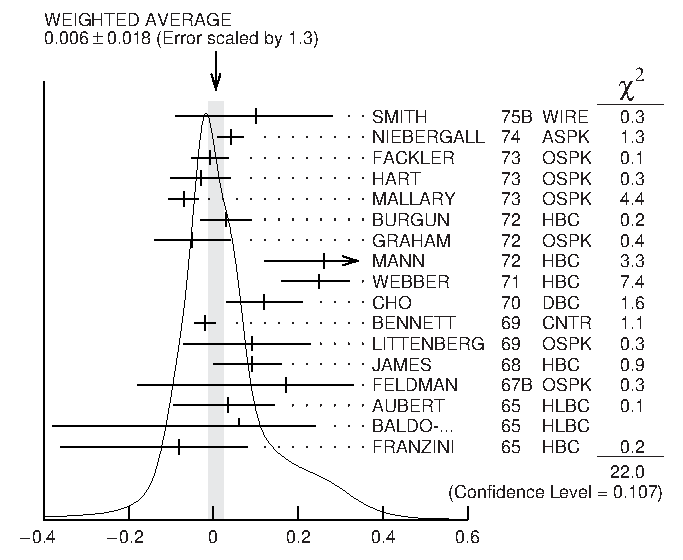
\includegraphics{filename} %multiple includegraphics may be used, 
	% with usual \hfill and \\ newline structures. 
\end{pdgxfigure}
\end{verbtex}

Figures placed in the \invt{figures} directory will be automaticallly found. 
Option keys may also be passed to individual \lstinline{\includegraphics} commands,  
as usual, if separate control is desired of multiple \lstinline{\includegraphics} in the same \invt{pdgxfigure} environment.
I.e. \lstinline!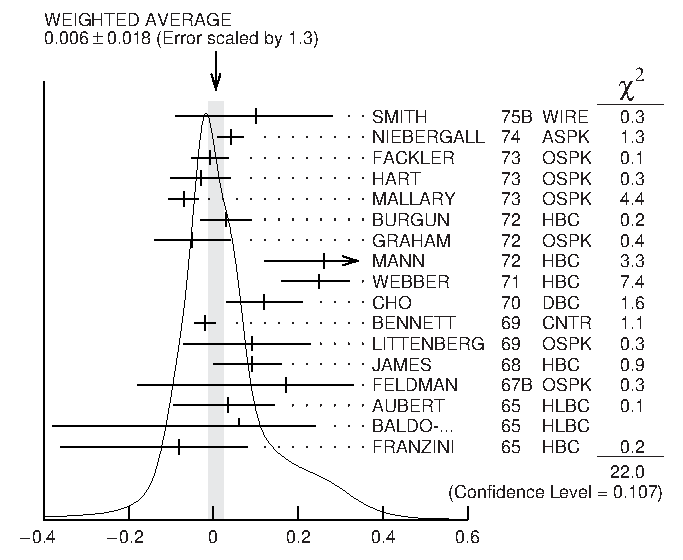
\includegraphics[<option keys>]{filename}!.

\Isubsection{Float scaling and width keys}
\label{sec:ginkeys}
As in the usual implementation of the \invt{graphicx} package, the \lstinline{\includegraphics} command takes optional standard keys \invt{width = ...}, \invt{scale = ...}.
which are used to control the width or scale of the bounding box. 
We use the same key structure to pass options to the \invt{pdgxfigure} environment, as well as to the \invt{pdgxtable} environment (see Sec.~\ref{sec:tables}).

The version specific keys \lstinline!<version>width! and \lstinline!<version>scale! have been added, 
that implement width or scaling choices only in the specific \invt{<version>}.
One may use these keys in concert with the usual \invt{width} and \invt{scale} keys, with the caveat that the order of keys matters: 
Keys are read left to right, and rightwards keys typically override leftwards ones. 
For example, passing the option keys (to either \invt{pdgxfigure} or \invt{pdgxtable}, or \lstinline{\includegraphics})
\begin{verbtex}
	[width=0.8\linewidth, bookwidth=0.9\linewidth]
\end{verbtex}
implements the \invt{width} key setting except in the book version. 
The option \lstinline!bookwidth=0.9\linewidth! followed by
\lstinline!width=0.8\linewidth! would instead implement only the version-general \lstinline!width=0.8\linewidth! setting.

\textbf{Note:} Because of specialization of the \invt{graphicx} key structure in the PDG class,
to use a \invt{scale} or \invt{<version>scale} key in an \lstinline{\includegraphics} command or \invt{pdgxfigure} environment
one must first pass an option key \invt{width=!}. This is not required for  \invt{pdgxtable}.

An additional key \lstinline!<version>bbscale! scales the float bounding box.
For some overwide floats that are larger than the nominal page width---in particular, overwide tables, see Sec.~\ref{sec:tables}---simply 
rescaling down the float does not allow it to be properly aligned on the page.
This key can be increased above $1$ (the default), to provide a sufficiently large bounding box for the float, that may then be scaled down to size with correct alignment.

\Isubsection{Available keys for \invt{pdgxfigure}}
Following is a list of available optional keys for \invt{pdgxfigure}, and default settings if not invoked.
As usual, keys are evaluated left to right. 
The version-general \invt{width} key can be used (and will override any preceeding version-specfic width key).
\begin{itemize}
	\item \invt{place}: Takes any combination of \invt{h}, \invt{t}, \invt{b}, \invt{p} (with optional \invt{\!}) that specifies float placement. Default is \invt{\!ht}.
	\item \invt{wide}: Takes \invt{true} or \invt{false} to specify the figure as full page width in either single or two column mode. Default is \invt{false}.
	\item \invt{width} or \invt{<version>width}: Sets the global or version specific width of the figure bounding box, respectively. Default is 0.75 of the line width (or text width, for wide figures).
	\item \invt{scale} or \invt{<version>scale}: Scales the figure according to float value passed to the key. 
	The option \lstinline{width=!} must be passed to turn off default width behavior and enable scaling keys.
\end{itemize}

\Isubsection{Examples}
The following produces a default-style, shown in Figure~\ref{examples:fig:example}. 
We recommend including the file extension in the \lstinline{\includegraphics} argument, to assist our editorial staff in addressing any figure quality problems.
\begin{verbtex}
\begin{pdgxfigure}[place=t] 
	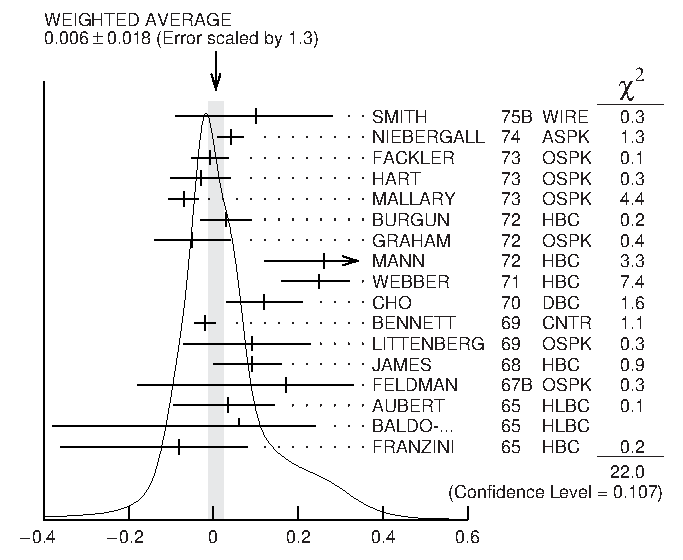
\includegraphics{filename.pdf}
	\caption{Example default figure}
	\label{examples:fig:example}
\end{pdgxfigure}
\end{verbtex}
\begin{pdgxfigure}[place=t]
	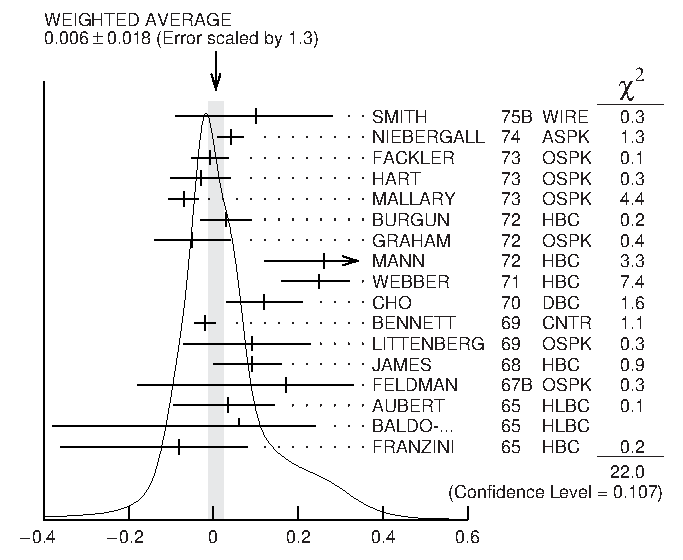
\includegraphics{filename.pdf}
	\caption{Example default figure}
	\label{examples:fig:example}
\end{pdgxfigure}

A double wide figure, shown in Fig.~\ref{examples:fig:example2}:
\begin{verbtex}
\begin{pdgxfigure}[wide=true,place=h, webwidth=0.45\linewidth, 
		bookwidth=0.9\linewidth] 
	%width key applies to all includegraphics instances
	%compiling in different versions will produce different widths
	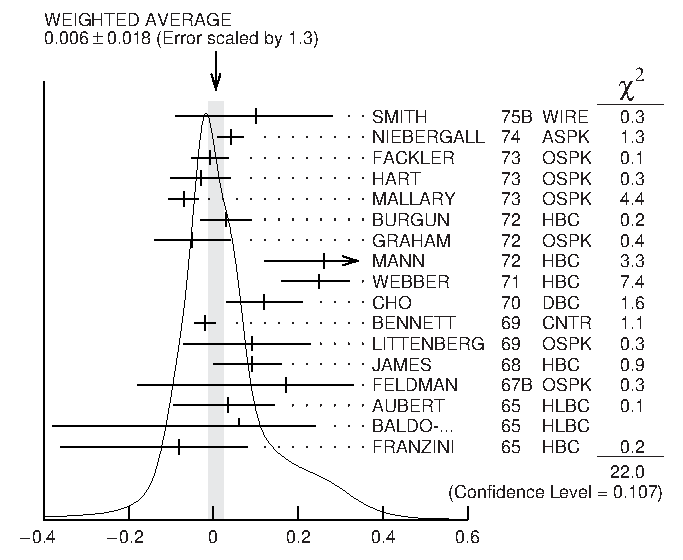
\includegraphics{filename.pdf}\hfill
	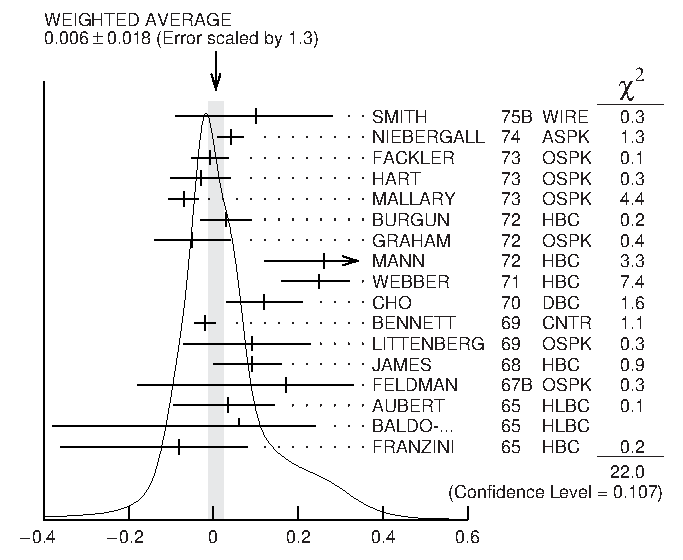
\includegraphics{filename.pdf}
	\caption{Example double wide figure, 
		with different book and web versions}
	\label{examples:fig:example2}
\end{pdgxfigure}
\end{verbtex}
\begin{pdgxfigure}[wide=true,place=h,width=0.45\textwidth] 
	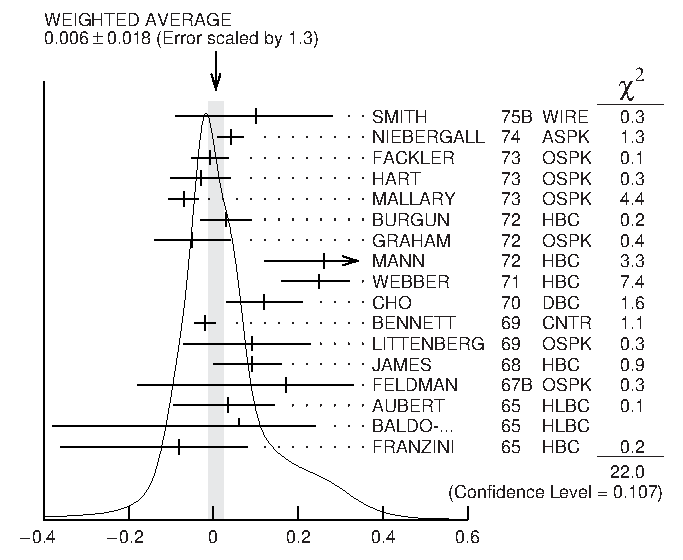
\includegraphics{filename.pdf}\hfill
	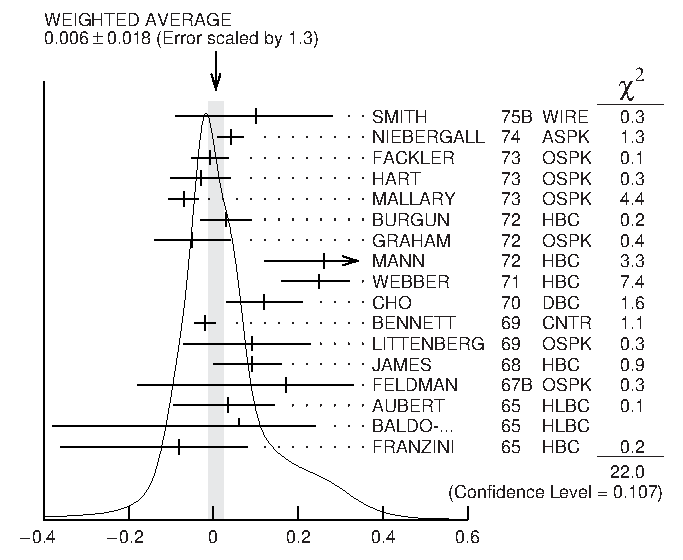
\includegraphics{filename.pdf}
	\caption{Example double wide figure, with different book and web versions}
	\label{examples:fig:example2}
\end{pdgxfigure}

A double wide figure with separate option and scaling keys, shown in Fig.~\ref{examples:fig:example3}:
\begin{verbtex}
\begin{pdgxfigure}[wide=true,place=h,width = 0.3\linewidth] 
	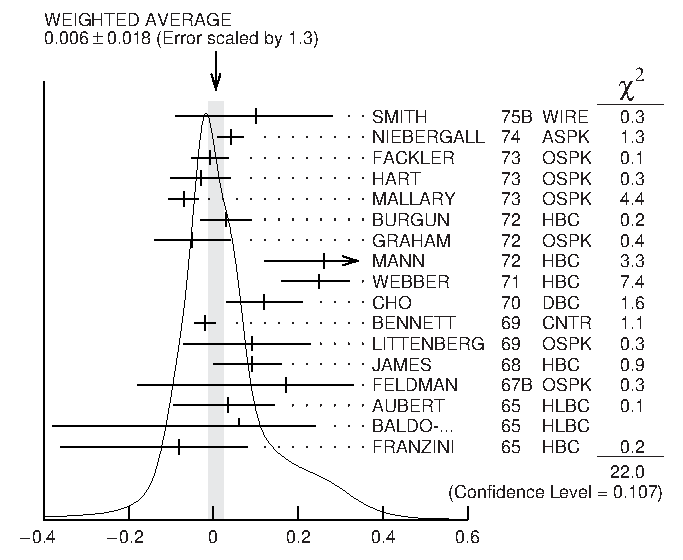
\includegraphics{filename.pdf}\hspace{1cm}
	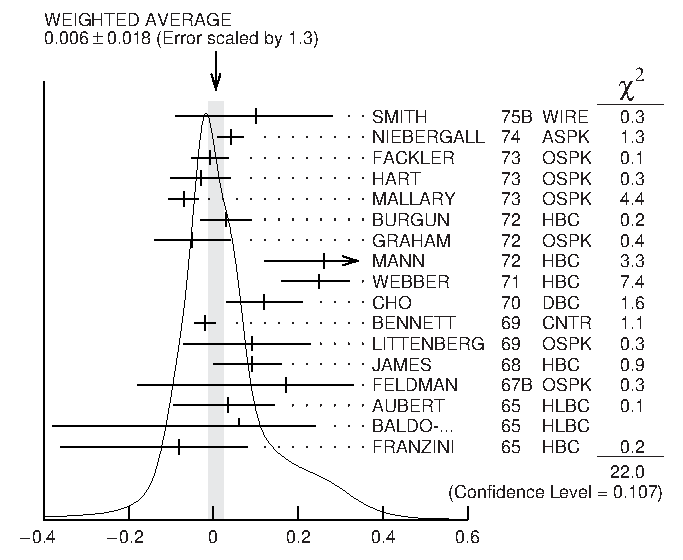
\includegraphics[width = !,scale =0.3,angle = 90]{filename}
	\caption{Example double figure, 
		with separate option and scaling keys, in both book and web versions}
	\label{examples:fig:example3}
\end{pdgxfigure}
\end{verbtex}
\begin{pdgxfigure}[wide=true,place=h,width = 0.3\linewidth] 
	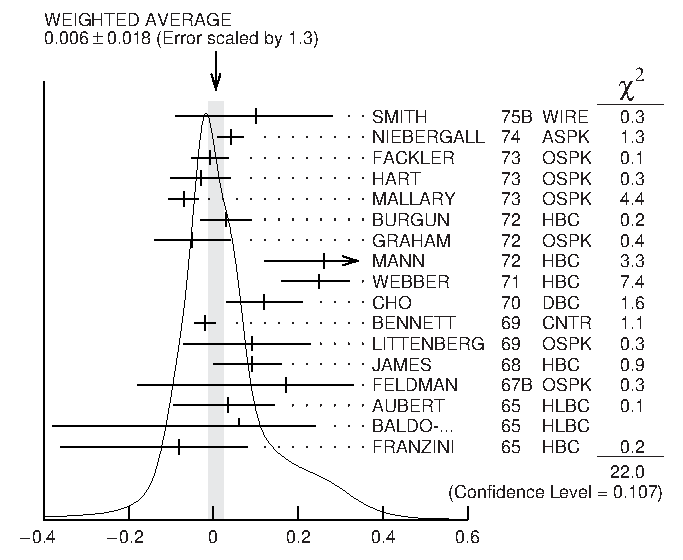
\includegraphics{filename.pdf}\hspace{1cm}
	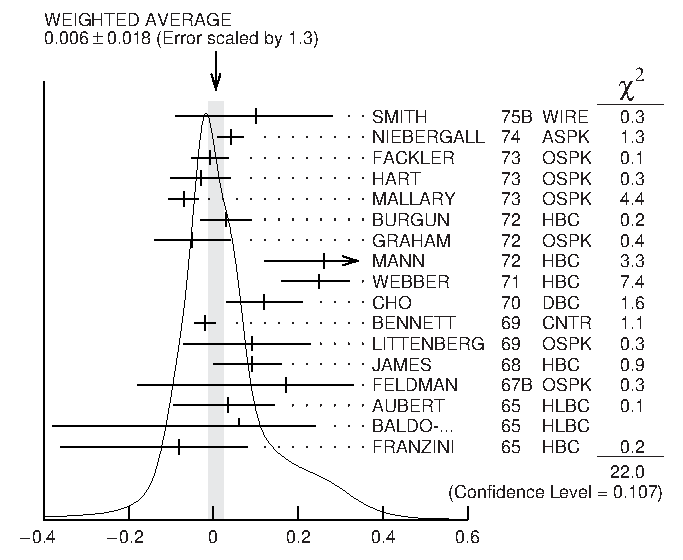
\includegraphics[width = !,scale =0.3,angle = 90]{filename}
	\caption{Example double wide figure, with separate option and scaling keys, in both book and web versions}
	\label{examples:fig:example3}
\end{pdgxfigure}

\Isubsection{\invt{pdgfigure} commands}
To add a figure, one may also use the \lstinline{\pdgfigure} or \lstinline{\pdgwidefigure} commands 
to typeset a single-column figure or double-column wide figure (for the book version), respectively. 
To include two images in one figure one may use \lstinline{\pdgdoublefigure}.
These commands are less powerful than \invt{pdgxfigure}, but automatically incorporate all PDG styles.

The macros \lstinline{\pdgfigure} and \lstinline{\pdgwidefigure} take the following arguments:
\begin{verbtex}
	\pdgfigure{<filename>}
	{<caption>}{<label>}{<placement options>}
	{<other option keys>}
\end{verbtex}
\vspace{-10pt}
while the macro \lstinline{\pdgdoublefigure} takes the following arguments:
\begin{verbtex}
	\pdgdoublefigure{<filename1>}{<filename2>}
	{<caption>}{<label>}{<placement options>}
	{<other option keys>}
\end{verbtex}
Some examples of the \invt{pdgfigure} commands are shown in Figs.~\ref{examples:fig:ideogram1}, \ref{examples:fig:ideogram2} and \ref{examples:fig:ideogram3}, respectively:
\begin{verbtex}
	\pdgfigure{filename.pdf}{Figure with caption and label}
	{examples:fig:ideogram1}{ht!}{}
	
	\pdgdoublefigure{filename.pdf}{filename.pdf}
	{Two figures, with caption and label, reduced in size}
	{examples:fig:ideogram2}{ht!}{width=0.3\textwidth}
	
	\pdgwidefigure{filename.pdf}{Wide figure}
	{examples:fig:ideogram3}{t}{}
\end{verbtex}
\FloatBarrier
\pdgfigure{filename.pdf}{Figure with caption and label}{examples:fig:ideogram1}{ht!}{}
\pdgdoublefigure{filename.pdf}{filename.pdf}{Two figures, with caption and label, reduced in size}{examples:fig:ideogram2}{ht!}{width=0.3\textwidth}
\pdgwidefigure{filename.pdf}{Wide figure}{examples:fig:ideogram3}{t}{}
\FloatBarrier

\Isection{Tables}
\label{sec:tables}
\Isubsection{ \invt{pdgxtable} and \invt{pdgxtabular}}
The PDG class provides multipurpose table and tabular environments, \invt{pdgxtable} and \invt{pdgxtabular}. 
These operate similarly to the standard \invt{table} and \invt{tabular} environments: \invt{(pdgx)table} creates a floating environment, 
while \invt{(pdgx)tabular} creates the actual tabulated display. 

The \lstinline!\caption! and \lstinline!\label! commands may be used as in the usual \invt{table} environment.
\textbf{Note: A table caption should be placed above the table.}
In addition, \invt{pdgxtable} takes a wide array of additional option keys that implement features and formatting of the prior PDG table commands/environments.  
These include keys that control placement, multicolumn spanning, version-specific widths and scaling (see Sec.~\ref{sec:ginkeys}), rotation, stretching, and caption widths.
The generic usage is
\begin{verbtex}
\begin{pdgxtable}[<option keys>]
	\caption{This is a PDG table}
	\label{tab:label}
	\begin{pdgxtabular}{<column settings>} % the usual c, l, r, | etc
		\pdgtableheader{...} %column header & separated entries go here
		%table & separated entries go here
	\end{pdgxtabular}
	%multiple pdgtabular environments are allowed
\end{pdgxtable}
\end{verbtex}

As for the usual \invt{table} environment, one may include multiple \invt{pdgxtabular}s in a single \invt{pdgxtable}.
While the \invt{pdgxtable} environment has default handling for caption widths in wide and regular tables, for both book and web versions, 
absolute control of the caption width can be implmented with a \lstinline{\captionsetup} command inside the \invt{pdgxtable} environment. 
For example \lstinline!\captionsetup{width=\linewidth}! gives a full width caption.

\Isubsection{Available keys for \invt{pdgxtable}}
Following is a list of available optional keys, and default settings if not invoked.
As usual, keys are evaluated left to right. 
While, the version-general \invt{width} key can be used (and will override any preceeding version-specfic width key), 
there is no version-general \invt{scale} key. 
Scaling of the tables is best done with the \invt{<version>scale} keys.

\begin{itemize}
	\item \invt{place}: Takes any combination of \invt{h}, \invt{t}, \invt{b}, \invt{p} (with optional \invt{\!}) that specifies float placement. Default is \invt{\!ht}.
	\item \invt{wide}: Takes \invt{true} or \invt{false} to specify the table as full page width in either single or two column mode. Default is \invt{false}.
	\item \invt{width} or \invt{<version>width}: Sets the version specific maximum width of the table bounding box. 
	Default is the maximum text width implied by the \invt{wide} key setting.
	Width settings exceeding this default are ineffective. Footnotes are scaled, but caption width is not affected.
	\item \invt{<version>scale}: Scales the table according to float value passed to the key. 
	For overwide tables, there is always a value $<1$ at which the table will be properly set to maximum page width.
	Footnotes are scaled, but caption width is not affected. Note the global \invt{scale} is disabled for \invt{pdgxtable}.
	\item \invt{<version>bbscale}: Scales the bounding box of the table. 
	For some overwide tables that are larger than the nominal page width, simply rescaling down the table does not allow the table to be properly aligned on the page.
	This key can be increased above $1$ (the default), to provide a sufficiently large bounding box for the table, that may then be scaled down to size with correct alignment.
	\item \invt{widecaptionscale}: For \invt{wide = true} tables, scales the caption width with respect to the maximum page width. Default is $0.75$.
	\item \invt{narrowcaptionscale}: For \invt{wide = false} or default tables, scales the caption width with respect to the maximum column width. Default is $0.9$.
	\item \invt{rotated}: Takes \invt{left} or \invt{right} to rotate the table, but not the caption, $90^\circ$ anticlockwise or clockwise, respectively. 
	The caption may be rotated independently, as needed with a \lstinline{\rotatebox}.
	\item \invt{sideways}: Takes \invt{true} or \invt{false} to rotate the table, including the caption, $90^\circ$ anticlockwise or clockwise, 
	according to whether the page number is even or odd.
	In a sideways table, other key width and scaling settings are still effective, but scale with respect to the page height. 
\end{itemize}


\Isubsection{Examples}
Some (simple) examples of \invt{pdgxtable} can be found in Table~\ref{examples:tab:styles} and Sec~\ref{sec:macros}.
For example, Tab.~\ref{examples:tab:styles} is typeset as
\begin{verbtex}
\begin{pdgxtable}[place=h,bookscale = 0.9,bookbbscale=2]
	\caption{Styles for the different typesetting versions}
	\label{examples:tab:styles}
	\begin{pdgxtabular}{ccccc}
		Version 		& Columns  & Font size 	& Helper Tags\footnote{
			Tags for each equation, table, figure, and bibliography entry 
			are displayed in margin or interspaced} & Line numbers\\
		\hline
		draft	& 1		   & 11pt		& Yes & Yes \\
		...
	\end{pdgxtabular}
\end{pdgxtable}
\end{verbtex}

Tables~\ref{examples:tab:commu} and~\ref{examples:tab:commp} are typeset as a two \invt{pdgxtabular}s in a single \invt{pdgxtable}, via
\begin{verbtex}
\begin{pdgxtable}[wide=true, place=!ht, webscale = 0.8]
	\caption{Common units}
	\label{examples:tab:commu}
	\begin{pdgxtabular}{lr | lr | lr}
		\showsymbol{\TeV} &  \showsymbol{\syin} & \showsymbol{\barn}   \\
		...
	\end{pdgxtabular}
	\caption{Common particles}
	\label{examples:tab:commp}
	\begin{pdgxtabular}{lr | lr | lr}
   		\showsymbol{\pp} &  \showsymbol{\ee} & \showsymbol{\pizero}   \\
  		...
	\end{pdgxtabular}
\end{pdgxtable}
\end{verbtex}

\Isubsection{Common problems and recommendations}
The \invt{pdgxtabular} environment is capable of handling the usual \lstinline{\multicolumn} and \lstinline{\multirow} objects, 
that allow for more complicated tables with cells spanning multiple rows and/or columns. 
We recommend avoiding use of \lstinline{\multispan}. 
For multiline cells, the \lstinline{\makecell} command from the \invt{makecell} package is recommended.

\Isection{Labels and referencing}
\label{sec:labels}

\Isubsection{Style guide}
As usual, the \lstinline{\label} and \lstinline{\ref} commands (and their derivatives) may be used to reference equations, tables, figures, and so on. 
To permit easy cross-referencing throughout the entire review, we request that you use the following labelling convention: \invt{BASENAME:type:name}
with \invt{type} corresponding to one of the following options
\begin{itemize}
\item {\tt fig} for figures
\item {\tt eq } for equation
\item {\tt tab} for tables
\item {\tt sec} for section, subsection etc..
\item {\tt foot} for footnotes.
\end{itemize}

\Isubsection{Missing references}

In default LaTeX, missing references are typically typeset as ``\textbf{??}''. 
To improve the typesetting experience, the \lstinline{\ref} command has been modified in the PDG class so that missing reference keys are printed out explicitly: 
For instance, a \lstinline!\ref{eqn:name}! that references a missing label called \invt{eqn:name}, will display as \ref{eqn:name}.
Similarly, the \lstinline{\cite} command will explicitly print out missing citation references. E.g. 
a \lstinline!\cite{name:2021ab}! that references a missing label called \invt{name:2021ab}, will display as \cite{name:2021ab}

\Isubsection{Cross-review referencing}
It is occasionally necessary or useful to reference (sub)sections, equations, figures, tables and so on belonging to other reviews or other reviews themselves. 
\textbf{Note:} Please use the \lstinline{\crossref} command for cross-review referencing.

Implementing a cross-reference to another review requires knowledge of its  \invt{BASENAME}:  
You must use the \invt{BASENAME} associated with the target review, not the \invt{BASENAME} of the review you're currently working on. 
To identify the  \invt{BASENAME} of another review, login into the \href{https://pdgworkspace.lbl.gov/Reviews.action}{PDG Workspace} (click to be redirected). 
Under \emph{Reviews} select from the drop-down menu \emph{All reviews}. 
Click on the title of the review you are interested in, and then select the \emph{Technical details} tab. 
The \invt{BASENAME} is the first entry.


If the full \invt{BASENAME:type:name} reference is known, you may include it with the usage \\
\lstinline!\crossref{BASENAME:type:name}!. 
This will typeset in your document as ``\crossref{BASENAME:type:name}'', because your local auxiliary files do not have the reference information of the other review.
PDG editorial staff will implement the cross-reference properly, when your review is prepared for production.

If the \invt{BASENAME:type:name} reference is not known, or the authors of the other review did not label the obect that you wish to reference, 
you may instead provide any descriptive argument to \lstinline{\crossref}. 
For example, \lstinline!\crossref{Equation 34.1.10}!.  
PDG editorial staff will implement the cross-reference properly, when your review and the other review are prepared for production.

\Isubsection{Booklet labeling and referencing}
If your review has a booklet version, it needs to be prepared at the same time as you prepare your full review.
The content to be displayed in the booklet needs to be included in \invt{BASENAME-booklet.tex}. 

The numerical tags for equations, tables, and figures in the booklet version of a review should match the tags in the full version. 
This can be achieved automatically in the booklet version by using a \lstinline!\tag{\ref{BASENAME:type:name}}! construction instead of \lstinline{\label}
to refer to the reference in the full version.
For example, if the full version has a labelled equation
\begin{verbtex}
\begin{equation}
	\label{BASENAME:eq:name}
	...
\end{equation}
\end{verbtex}
then including in \invt{BASENAME-booklet.tex}
\begin{verbtex}
\begin{equation}
	\tag{\ref{BASENAME:eq:name}}
	...
\end{equation}
\end{verbtex}
will automatically label the equation correctly. 
To achieve the same result for figures and tables, one may place in the booklet version
\begin{verbtex}
	\renewcommand{\thetable}{\ref{BASENAME:type:name}}
	\renewcommand{\thefigure}{\ref{BASENAME:type:name}}
\end{verbtex}
before each table or figure environment, respectively. 


\Isection{Index entries}
\label{sec:index}

Review authors should think about any keywords that should be included into the index of the Review of Particle Physics. PDG uses the standard \LaTeX\  \invt{makeidx} package. Thus an entry ``sample text'' can be added to the index by placing
\begin{verbtex}
\index{sample text}
\end{verbtex}
at the appropriate place in the source file. Formatting of entries with Greek letters or math symbols as well as subentries are also supported. For example
\begin{verbtex}
\index{sigma@$\$$\sigma$\$$} 
\end{verbtex}
creates an index entry $\sigma$ in the proper alphabetical order, while
\begin{verbtex}
\index{Searches!Axion searches} 
\end{verbtex}
produces a subentry ``Axion searches'' under the ``Searches'' index entry.

All index entries defined in a given review will be shown on the last page when the draft version is made. PDG staff will standardize all index entries during the final processing of all reviews. Therefore what matters is not the final formatting of index entries but that all relevant entries are added in the correct place.


\Isection{Bibliography}
\label{sec:cites}

Citations are handled using BibTeX. To add a citation to your review:
\begin{itemize}
\item Look up the reference in INSPIRE and download its BibTeX entry (see bottom of the \emph{Information} tab for the article, under \emph{Export}).
\item Add the BibTeX entry to the \invt{BASENAME.bib} file. Note the article tag assigned by INSPIRE: You can see it in the first line of the BibTeX entry, after \lstinline!@article{!.
\item Cite the reference with \lstinline{\cite}, using the article tag assigned by INSPIRE.
\end{itemize}

For example, to add a reference to the Review of Particle Physics (2018) 
add the following code to \invt{BASENAME.bib}:
\begin{verbtex}
@article{Tanabashi:2018oca,
      author         = "Tanabashi, M. and others",
      title          = "{Review of Particle Physics}",
      collaboration  = "Particle Data Group",
      journal        = "Phys. Rev.",
      volume         = "D98",
      year           = "2018",
      number         = "3",
      pages          = "030001",
      doi            = "10.1103/PhysRevD.98.030001",
      SLACcitation   = "%%CITATION = PHRVA,D98,030001;%%"
 }
\end{verbtex}
and then one may add a reference to it in \invt{BASENAME-main.tex} via \lstinline!\cite{Tanabashi:2018oca}!.

If a BibTeX entry downloaded from INSPIRE does not render correctly, 
you should first make sure you have the latest PDG style files, by running \invt{svn update} (after committing any edits you have made).
If this doesn't fix the issue please contact \invt{latexsupport@pdg.lbl.gov} for advice.  
If it appears, however, to be simply a mistake in INSPIRE's entry, 
rename the label to the form \invt{BASENAME:<INSPIRE label>} and then edit the entry as needed.
\textbf{Please do not edit entries downloaded from INSPIRE without changing the label.}
Changing the label will permit PDG editorial staff to easily identify and track edited citations, as well as notify INSPIRE of required corrections.
In case the reference does not appear in INSPIRE at all, please also use the convention for the label: \invt{BASENAME:name}.

Multiple references can be added to a single set of brackets with \lstinline!\cite{cite-key-1,cite-key-2,...}!.
One may group multiple references into the same numerical citation tag, using a \invt{*} prefix on subsequent citation keys: For example \lstinline!\cite{cite-key-1,*cite-key-2,*cite-key-3}!.
If a paper citation key is preceded by the asterisk, it can't be cited separately later, and doing so will result in a compilation error.
We recommend citing papers individually, without using the asterisk to group them.


\Isection{Footnotes}
Footnote styles are standardized throughout the review. In (rare) cases that the style needs to be changed, this is achieved via \lstinline!\setfootnotestyle{<style>}!,
where \invt{<style>} can be \lstinline{\fnsymbol} or \lstinline{\alph}, \lstinline{\Alph}, \lstinline{\arabic}, \lstinline{\roman}, \lstinline{\Roman} etc.

Sometimes the \LaTeX \ engine miscalculates the amount of space required for a footnote, resulting in overprinting of the footer.
One can help the engine obtain a better estimate by adjusting the effective page size. 
This can be done by placing \lstinline!\enlargethispage{-2\baselineskip}! somewhere just before the \lstinline{\footnote}; the \invt{-2} may be changed to any number. 

\Isection{Miscellaneous control commands}

\Isubsection{Unbalanced last page}
In the book version, the columns of the final page are automatically balanced. 
If this behavior is undesired, it may be altered by invoking \lstinline!\balancedlastpagefalse!.
The invocation may be added anywhere in the document.

\Isubsection{Blank last page}
In the book version, a blank final page may be added via \lstinline!\blankendpagetrue!.
The invocation may be added anywhere in the document.

\Isubsection{Book-only reviews}
Certain reviews are typeset for the web using the book version formatting. 
This is enforced automatically within the PDG system by \lstinline!\def\iswebbook{1}! before the \lstinline{\documentclass} invocation. 
The draft version, however, for such reviews are typeset in the usual draft/web format.

\clearpage
\Isection{PDG Macros}
\label{sec:macros}

\begin{pdgxtable}[wide=true, place=!ht, webscale = 0.8]
	\vspace{-10pt}
	\caption{Common units}
	\label{examples:tab:commu}
	\begin{pdgxtabular}{lr | lr | lr}
		\showsymbol{\TeV     } &  \showsymbol{\syin} & \showsymbol{\barn     }   \\
		\showsymbol{\MeV     } &  \showsymbol{\inch} & \showsymbol{\mbarn    }   \\
		\showsymbol{\keV     } &  \showsymbol{\ft  } & \showsymbol{\microbarn}   \\
		\showsymbol{\eV      } &  \showsymbol{\km  } & \showsymbol{\nb       }   \\
		\showsymbol{\GeVc    } &  \showsymbol{\m   } & \showsymbol{\pb       }   \\
		\showsymbol{\GeVcSq  } &  \showsymbol{\cm  } & \showsymbol{\fb       }   \\
		\showsymbol{\GeVcc   } &  \showsymbol{\mm  } & \showsymbol{\invnb    }   \\
		\showsymbol{\GeVccSq } &  \showsymbol{\mum } & \showsymbol{\invpb    }   \\
		\showsymbol{\MeVc    } &  \showsymbol{\nm  } & \showsymbol{\invfb    }   \\
		\showsymbol{\MeVcc   } &  \showsymbol{\fm  } & \showsymbol{\invab    }   \\
		\showsymbol{\invps   } &  \showsymbol{\nm  } & \showsymbol{\lum      }   \\
			&&  \showsymbol{\ma  } &&  \\
		\showsymbol{\degr    }  &  \showsymbol{\cma } && \\
			&&  \showsymbol{\mma } &&   \\
			&&  \showsymbol{\muma} &&   \\
	\end{pdgxtabular}
	\vspace{10pt}
	\caption{Common particles}
	\label{examples:tab:commp}
	\vspace{-10pt}
	\begin{pdgxtabular}{lr | lr | lr}
   \showsymbol{\pp         } &  \showsymbol{\ee           } & \showsymbol{\pizero   }   \\
   \showsymbol{\pbar       } &  \showsymbol{\epm          } & \showsymbol{\piplus   }   \\
   \showsymbol{\ppbar      } &  \showsymbol{\epem         } & \showsymbol{\piminus  }   \\
   \showsymbol{\tbar       } &  \showsymbol{\en           } & \showsymbol{\pipm     }   \\
   \showsymbol{\ttbar      } &  \showsymbol{\ep           } & \showsymbol{\pimp     }   \\
   \showsymbol{\bbar       } &  \showsymbol{\mumu         } & \showsymbol{\etaprime }   \\
   \showsymbol{\bbbar      } &  \showsymbol{\mun          } & \showsymbol{\Kzero    }   \\
   \showsymbol{\cbar       } &  \showsymbol{\mup          } & \showsymbol{\Kzerobar }   \\
   \showsymbol{\ccbar      } &  \showsymbol{\tautau       } & \showsymbol{\kaon     }   \\
   \showsymbol{\sbar       } &  \showsymbol{\taup         } & \showsymbol{\Kplus    }   \\
   \showsymbol{\ssbar      } &  \showsymbol{\taum         } & \showsymbol{\Kminus   }   \\
   \showsymbol{\ubar       } &  \showsymbol{\lepton       } & \showsymbol{\KzeroL   }   \\
   \showsymbol{\uubar      } &  \showsymbol{\leptonm      } & \showsymbol{\Kzerol   }   \\
   \showsymbol{\dbar       } &  \showsymbol{\ellm         } & \showsymbol{\Klong    }   \\
   \showsymbol{\ddbar      } &  \showsymbol{\leptonp      } & \showsymbol{\KzeroS   }   \\
   \showsymbol{\fbar       } &  \showsymbol{\ellp         } & \showsymbol{\Kzeros   }   \\
   \showsymbol{\ffbar      } &  \showsymbol{\leptonlepton } & \showsymbol{\Kshort   }   \\
   \showsymbol{\qbar       } &  \showsymbol{\ellell       } & \showsymbol{\Kstar    }   \\
   \showsymbol{\qqbar      } &  \showsymbol{\enu          } & \showsymbol{\jpsi     }   \\
   \showsymbol{\nbar       } &  \showsymbol{\munu         } & \showsymbol{\Jpsi     }   \\
   \showsymbol{\nnbar      } &  \showsymbol{\taunu        } & \showsymbol{\psip     }   \\
   \showsymbol{\neutron    } &  \showsymbol{\lnu          } & \showsymbol{\chic     }   \\
   \showsymbol{\antineutron} &  \showsymbol{\nub          } & \showsymbol{\UoneS    }   \\
   \showsymbol{\deuteron   } &  \showsymbol{\nunub        } & \showsymbol{\chib     }   \\
   \showsymbol{\Zzero      } &  \showsymbol{\nue          } & \showsymbol{\Dstar    }   \\
   \showsymbol{\Zboson     } &  \showsymbol{\nueb         } & \showsymbol{\Bd       }   \\
   \showsymbol{\Wplus      } &  \showsymbol{\nuenueb      } & \showsymbol{\Bs       }   \\
   \showsymbol{\Wminus	   } &  \showsymbol{\num          } & \showsymbol{\Bu       }   \\
   \showsymbol{\Wboson	   } &  \showsymbol{\numb         } & \showsymbol{\Bc       }   \\ 
   \showsymbol{\Wpm   	   } &  \showsymbol{\numnumb      } & \showsymbol{\Lb       }   \\
   \showsymbol{\Wmp        } &  \showsymbol{\nut          } & \showsymbol{\Bstar    }   \\
   \showsymbol{\Hzero } &  \showsymbol{\nutb         } & \showsymbol{\BoBo     }   \\
   \showsymbol{\Hboson}  &	\showsymbol{\nutnutb      } & \showsymbol{\BodBod   }    \\		    
   \showsymbol{            } &	\showsymbol{              } & \showsymbol{\BosBos   }    \\		    
   \showsymbol{            } &	\showsymbol{              } & \showsymbol{\LambdaStar}  \\
	\end{pdgxtabular}
\end{pdgxtable}

\begin{pdgxtable}[wide=true, place=h, webscale = 0.8]
	\caption{Hypothetical particles}
	\begin{pdgxtabular}{lr | lr | lr}
   \showsymbol{\Azero }      &  \showsymbol{\gravino   } & \showsymbol{\slepton   }   \\
   \showsymbol{\hzero }      &  \showsymbol{\Zprime    } & \showsymbol{\sleptonL  }   \\
   \showsymbol{\Hzero }      &  \showsymbol{\Zstar     } & \showsymbol{\sleptonR  }   \\
   \showsymbol{\Hplus }  	  &  \showsymbol{\squark    } & \showsymbol{\sel       }   \\
   \showsymbol{\Hminus}       &  \showsymbol{\squarkL   } & \showsymbol{\selL      }   \\
   \showsymbol{\Hpm   }   	&  \showsymbol{\squarkR   } & \showsymbol{\selR      }   \\
   \showsymbol{\Hmp   }       &  \showsymbol{\gluino    } & \showsymbol{\smu       }   \\
   \showsymbol{\ggino }     &  \showsymbol{\stop      } & \showsymbol{\smuL      }   \\
   \showsymbol{\chinop}      &  \showsymbol{\stopone   } & \showsymbol{\smuR      }   \\
   \showsymbol{\chinom}      &  \showsymbol{\stoptwo   } & \showsymbol{\stau      }   \\
   \showsymbol{\chinopm}      &  \showsymbol{\stopL     } & \showsymbol{\stauL     }   \\
   \showsymbol{\chinomp}     &  \showsymbol{\stopR     } & \showsymbol{\stauR     }   \\
   \showsymbol{\chinoonep}     &  \showsymbol{\sbottom   } & \showsymbol{\stauone   }   \\
   \showsymbol{\chinoonem}   &  \showsymbol{\sbottomone} & \showsymbol{\stautwo   }   \\
   \showsymbol{\chinoonepm}   &  \showsymbol{\sbottomtwo} & \showsymbol{\snu       }   \\
   \showsymbol{\chinotwop}  &  \showsymbol{\sbottomL  } & \showsymbol{           }   \\
   \showsymbol{\chinotwom}   &  \showsymbol{\sbottomR  } & \showsymbol{           }   \\
   \showsymbol{\chinotwopm}   &  \showsymbol{           } & \showsymbol{           }   \\
   \showsymbol{\nino}  &  \showsymbol{           } & \showsymbol{           }   \\
   \showsymbol{\ninoone}        &  \showsymbol{           } & \showsymbol{           }   \\
   \showsymbol{\ninotwo}     &  \showsymbol{           } & \showsymbol{           }   \\
   \showsymbol{\ninothree}     &  \showsymbol{           } & \showsymbol{           }   \\
   \showsymbol{\ninofour}   &  \showsymbol{           } & \showsymbol{           }   \\
	\end{pdgxtabular}
\vspace*{10pt}
	\caption{Useful symbols for proton-proton physics}
\vspace*{-10pt}	
	\begin{pdgxtabular}{lr | lr }
   \showsymbol{\pT  }      &  \showsymbol{\rts }   \\
   \showsymbol{\pt  }      &  \showsymbol{\sqs } \\
   \showsymbol{\ET  }      &  \showsymbol{\mh}  \\
   \showsymbol{\eT  }      &  \showsymbol{\mW}  \\
   \showsymbol{\et  }      & \showsymbol{\mZ}   \\
   \showsymbol{\HT  }      & \showsymbol{\mH}   \\
   \showsymbol{\pTsq}      &&   \\
   \showsymbol{\MET }      &&   \\
   \showsymbol{\met }      &&   \\
   \showsymbol{\Ecm }      &&   \\
	\end{pdgxtabular}
\vspace*{10pt}
	\caption{Monte Carlo Generators}
\vspace*{-10pt}		
	\begin{pdgxtabular}{lr | lr | lr}	
   \showsymbol{\ACERMC    }      &  \showsymbol{\MCatNLO   } & \showsymbol{\Comphep    }   \\
   \showsymbol{\ALPGEN    }      &  \showsymbol{\AMCatNLO  } & \showsymbol{\Prospino   }   \\
   \showsymbol{\GEANT     }      &  \showsymbol{\MCFM      } & \showsymbol{\LO         }   \\
   \showsymbol{\Herwigpp  }      &  \showsymbol{\METOP     } & \showsymbol{\NLO        }   \\
   \showsymbol{\HERWIGpp  }      &  \showsymbol{\POWHEG    } & \showsymbol{\NLL        }   \\
   \showsymbol{\Herwig    }      &  \showsymbol{\POWHEGBOX } & \showsymbol{\NNLO       }   \\
   \showsymbol{\HERWIG    }      &  \showsymbol{\POWPYTHIA } & \showsymbol{\muF        }   \\
   \showsymbol{\JIMMY     }      &  \showsymbol{\PROTOS    } & \showsymbol{\muR        }   \\
   \showsymbol{\MADSPIN   }      &  \showsymbol{\PYTHIA    } & \showsymbol{            }   \\
   \showsymbol{\MADGRAPH  }      &  \showsymbol{\SHERPA    } & \showsymbol{            }   \\
   \showsymbol{\MGMCatNLO }      &  \showsymbol{           } & \showsymbol{            }   \\
	\end{pdgxtabular}
\end{pdgxtable}

\Isection{Tables: Legacy commands}

Though no longer recommended, legacy \lstinline{\pdgtable} or \lstinline{\pdgwidetable} commands 
to typeset a single-column table or double-column wide table (for the book version), respectively.
The \lstinline{\pdgtableheader} macro may be used in the first line of the table to automatically typeset a header.

The macros \lstinline{\pdgtable} and \lstinline{\pdgwidetable} take the following arguments:
\begin{verbtex}
	\pdgtable{<column styles>}
	{<caption>}{<label>}{<option keys>}
\end{verbtex}
Some examples usages of these commands follow, in Tables~\ref{examples:tab:table1}, \ref{examples:tab:table2} and~\ref{examples:tab:table3} below.
\begin{verbtex}
\begin{pdgtable}{c c c} 
	{Table}{examples:tab:table1}{h!}
	\pdgtableheader{ Column 1 & Column 2 & Column 3}
	row1  & 1  & 2\\
	row2  & 1  & 2\\
	row3  & 1  & 2\\
\end{pdgtable}
\end{verbtex}   
\begin{verbtex}
\begin{pdgtable}{|c | c | c | c|} 
	{Multicolumn table}{examples:tab:table2}{h!}
	\pdgtableheader{ \multicolumn{2}{c}{Column 1} & 
	\multicolumn{2}{c}{Column 2}}
	\pdgtableheader{ A & B& C & D }
	row1  & 1 & 2 &3 \\
	row2  & 1 & 2 &3 \\
\end{pdgtable}
\end{verbtex}  
\begin{verbtex}
\begin{pdgtable}{c l}
	{Table with footnotes}{examples:tab:table3}{}
	One value & another\footnote{This is something to notice
	\label{kmmix:foot:one}}\\
	Two values\footref{kmmix:foot:one} & another \\
\end{pdgtable}
\end{verbtex} 
 
\FloatBarrier 
\begin{pdgtable}{c c c} 
{Table}{examples:tab:table1}{h!}
\pdgtableheader{ Column 1 & Column 2 & Column 3}
row1  & 1  & 2\\
row2  & 1  & 2\\
row3  & 1  & 2\\
\end{pdgtable}
\begin{pdgtable}{|c | c | c | c|} 
{Multicolumn table}{examples:tab:table2}{h!}
\pdgtableheader{ \multicolumn{2}{|c|}{Column 1} & 
\multicolumn{2}{|c|}{Column 2}}
\pdgtableheader{ A & B& C & D }
row1  & 1 & 2 &3 \\
row2  & 1 & 2 &3 \\
\end{pdgtable}
\begin{pdgtable}{c l}
{Table with footnotes}{examples:tab:table3}{}
One value & another\footnote{This is something to notice\label{kmmix:foot:one}}\\
Two values\footref{kmmix:foot:one} & another \\
\end{pdgtable}
! line that includes these instructions in the main source file of your review, \invt{databases-main.tex}.

This documentation focuses mostly on the specialized functionality of the PDG \LaTeX \ class: %There are many resources that provide more general guidance for typesetting in \LaTeX.
For further support, or any \LaTeX-related questions, we invite authors to contact
\vspace{-0.2cm}
\begin{center}
\scalebox{1.5}{
	\invt{latexsupport@pdg.lbl.gov}
}
\end{center}

\Isubsection{File structure}
The source files for a PDG review are kept in separate directories within a SVN repository. 
Some files in each directory are auto-generated, while others are designed to be edited by review authors. 
\textbf{Do not edit auto-generated files, as any edits to these files will be overwritten periodically.}

Each review is assigned a unique name ("basename") that is used to label the relevant review files and will be referred to as \invt{BASENAME} in the following. For example, the QCD review is assigned basename \invt{qcd}. Therefore \invt{BASENAME-main.tex} in this documentation refers to file \invt{qcd-main.tex} for the QCD review.

Your review is assigned basename \invt{databases}.

The basename is further used to label cross-references to the review (see Sec.~\ref{sec:labels}) and specialized citations (see Sec.~\ref{sec:cites}). 
The file structure of a typical review is as follows:
\begin{itemize}
\item \invt{BASENAME-main.tex} --- contains the text of your review. 
\item \invt{BASENAME-booklet.tex} --- contains the text of the booklet version of your review (if there is one)
\item \invt{BASENAME-preamble.tex} --- contains review-specific definitions or inclusion of packages, that need to go into the document's preamble
\item \invt{BASENAME.bib} --- BibTeX bibliography entries (see Sec~\ref{sec:cites})
\item \invt{/figures} --- directory containing all figures
\item Auxiliary files (\invt{.aux}, \invt{.out}, \invt{.log}) --- these are generated by the \LaTeX compiler
\item Other \invt{.tex} files --- may be added and included in \invt{BASENAME-main.tex} or \invt{BASENAME-booklet.tex} with the \lstinline{\input} command.
\item \textbf{[auto-generated]} \invt{BASENAME.tex} --- compilation file for the review
\item \textbf{[auto-generated]} \invt{Makefile} --- Makefile to compile the review automatically (see Sec.~\ref{sec:make})
\item \textbf{[auto-generated]} \invt{pdg.cls} --- PDG \LaTeX \ class file
\item \textbf{[auto-generated]} \invt{pdg.bst} --- BibTeX PDG style file
\item \textbf{[auto-generated]} \invt{pdg-xr-hyper.sty} --- helper BibTeX style file
\item \textbf{[auto-generated]} \invt{pdgdefs.tex} --- PDG standard symbols and macros
\item \textbf{[auto-generated]} \invt{examples.tex} --- This file
\end{itemize}

\begin{center}
~\\
%!%\vspace{-12pt}
%!%In your review, the basename is databases.
\end{center}
To identify the  \invt{BASENAME} of yours or another review, you may also login into the 
\href{https://pdgworkspace.lbl.gov/Reviews.action}{PDG Workspace} (click to be redirected). 
Under \emph{Reviews} select from the drop-down menu \emph{All reviews}. 
Click on the title of the review you are interested in, and then select the \emph{Technical details} tab. 
The \invt{BASENAME} is the first entry.

\Isubsection{Multiversion typesetting}
The PDG \LaTeX \ class has functionality to typeset in four different versions or styles: draft, web, book and booklet. 
(The draft and web versions are referred to below jointly as `web', since they are broadly similar). 
See Table~\ref{examples:tab:styles} for a broad summary.

\begin{pdgxtable}[place=h,bookscale = 0.9,bookbbscale=2]
	\caption{Styles for the different typesetting versions}
	\label{examples:tab:styles}
	\begin{pdgxtabular}{ccccc}
		Version 		& Columns  & Font size 	& Helper Tags\footnote{
			Tags for each equation, table, figure, and bibliography entry are displayed in margin or interspaced} & Line numbers\\
		\hline
		\invt{draft} 	& 1		   & 11pt		& Yes & Yes \\
		\invt{web} 		& 1		   & 11pt		& No  & No\\
		\invt{book} 	& 2		   & 8pt		& No  & No\\
		\invt{booklet} 	& 1		   & 8pt		& No & No \\
	\end{pdgxtabular}
\end{pdgxtable}

Specialized macros may also have version-specific implementations. 
These follow the naming convention \invt{<version><macroname>}, where \invt{<version>} may take values of \invt{book}, \invt{booklet} and \invt{web}.
See for example, Sec.~\ref{sec:align}.
Specialized option keys follow the same convention. See e.g. Sec.~\ref{sec:ginkeys}.


\Isubsection{Makefile}
\label{sec:make}
We recommend to compile the review using \invt{make} on the command line. The usage is as follows:
\begin{itemize}
	\item \invt{make} --- compiles in draft mode.
	\item \invt{make  <version>} --- compiles in \invt{<version>} mode. For example \invt{make web}.
	\item \invt{make bib} --- compiles only the BibTeX files.
	\item \invt{make clean} --- cleans out all auxiliary files.
	\item \invt{make cleanall} --- cleans out the compiled pdf and all auxiliary files.
	\item \invt{make prod} --- cleans all auxiliary files, then compiles the web version.
	\item {\footnotesize{\texttt{make crossref}}} --- compiles required cross-referencing files (advanced: requires checkout of the other reviews to be cross-referenced).
\end{itemize}



\Isection{Style guides}
\Isubsection{Particle symbols}
Particle symbols are italic (or slanted) characters: \en, \pbar, \Lb, \pizero, \Klong, \Dstar. 
Charge is indicated by a superscript: $B^{-}$, $\Delta^{++}$. 
Charge is not normally indicated for $p$, $n$, or the quarks, and is optional for neutral isosinglets: $\eta$ or $\eta^{0}$. 
Antiparticles and particles are distinguished by charge for
charged leptons and mesons: $\tau^{+}$, $\kaon^{-}$ 
Otherwise, distinct antiparticles are indicated by a bar (overline): $\nbar_{\mu}$, \tbar, \pbar, \Kzerobar.

\Isubsection{Macros and shortcuts}
The \invt{pdgdefs.tex} file implements a series of useful macros for particle symbols, units and other common notation. 
All definitions are terminated with  \lstinline!\string\xspace!, so you can simply write ``\lstinline!\ttbar production!'' to typeset inline ``\ttbar production''.
The entire list of macros is provided in Sec.~\ref{sec:macros}.

Most Monte Carlo generators have a macro with a suffix 'V' that allows you to include the version. E.g. \lstinline!\PYTHIAV{8.1}! produces \PYTHIAV{8.1}.
In case you need to define other symbols, please add them to the \invt{BASENAME-preamble.tex} file.

\Isubsection{Column switching}

The web version is typeset as single column, singleside 11pt style, the book as 8pt double column, double sided.

In all versions of the review, switching between single and double column mode can be done \emph{in situ} with \lstinline{\onecolumn} or \lstinline{\twocolumn}
respectively. For example

\medskip
\ifrppbook
	\onecolumn
\else
	\twocolumn
\fi
{\footnotesize{Lorem ipsum dolor sit amet, consectetur adipiscing elit. Duis congue lectus at lectus tristique porta. Vivamus scelerisque porta massa, laoreet pulvinar dolor blandit vitae. Nam rhoncus id risus in tincidunt. Maecenas ultrices, arcu id gravida tempor, urna libero sodales nunc, quis dapibus ipsum quam eget est. Quisque eget convallis odio, at pellentesque quam. Mauris pretium eu metus ac imperdiet. Class aptent taciti sociosqu ad litora torquent per conubia nostra, per inceptos himenaeos. Nulla quis tincidunt libero. Aliquam posuere at quam quis posuere. Etiam turpis nulla, faucibus eget massa sagittis, porttitor sagittis elit. Proin a lorem eleifend, rhoncus orci quis, mattis metus. Donec sit amet lobortis lacus. Quisque magna augue, elementum nec ipsum non, feugiat ultricies urna. Sed tincidunt nisl vestibulum leo finibus, vitae sollicitudin sapien bibendum. Duis maximus ipsum nec urna lobortis, sed scelerisque nulla facilisis. Sed id finibus libero. }}
\ifrppbook
	\twocolumn
\else
	\onecolumn
\fi
\medskip

\Isection{Equations}
Equations may be typeset using the \invt{equation}, \invt{array}, \invt{multline}, and \invt{gather} etc environments provided by \invt{amsmath} package. 
We do not recommend using \invt{eqnarray}. As a trivial example
\begin{verbtex}
\begin{equation}
\label{BASENAME:eq:equation}
	N_{exp} = \sigma_{exp} \times \int L(t) dt
\end{equation}
\end{verbtex}
which produces
\begin{equation}
	N_{exp} = \sigma_{exp} \times \int L(t) dt
\end{equation}


To tag a set of equations with a common numbering and label, please use the \invt{subequation} environment, together with \invt{align}.
As an example:
\begin{verbtex}
\begin{subequations}
	\label{BASENAME:eq:equation1}
	\begin{align}
		A + B = C\\
		D= \frac{E}{F}  
	\end{align}
\end{subequations}
\end{verbtex}
which produces
\begin{subequations}
\begin{align}
	A + B = C\\
	D= \frac{E}{F}  
\end{align}
\end{subequations}


\Isubsection{Wide equations: \invt{pdgstrip}}
Some wide equations are not easily amenable to display in the PDG book double column format. 
Similar to the ReVTeX \invt{widetext} environment, the PDG style provides a \invt{pdgstrip} environment, that may wrap any other equation (or align, array etc) environment. 
The \invt{pdgstrip} environment is not a float, and will respect absolute placement in the typesetting stream. 
For example:
\begin{verbtex}
	\begin{pdgstrip}
		\begin{equation} % or any other display environment
		...

		\end{equation}
	\end{pdgstrip}
\end{verbtex}
In the web and booklet versions, this environment performs no operation on the wrapped environment. 
In the book version, the equation is preserved as a single `strip' across both columns, with column-wide rules to guide the reader's eye. 
The column-wide rules may be disabled -- e.g if the strip environment falls at the top or bottom of a page --  by passing the option \invt{plain} to the \invt{pdgstrip} environment. I.e. 
\lstinline!\begin{pdgstrip}[plain]!.

In principle, the pdgstrip envirornment may also wrap a floating environment such as a figure. 
In the book version, this will disable the ability of the figure to float, and fix it to a desired location.

\Isubsection{Alignment}
\label{sec:align}
Within \invt{align} environments or any other environment that uses the special \invt{&} and \invt{\\\\} (or \lstinline{\cr}) control characters for alignment, one may use
use version specific \lstinline!\bookalign!, \lstinline!\webalign!, \lstinline!\bookletalign! and \lstinline!\bookcr!, \lstinline!\webcr!, \lstinline!\bookletcr! macros.

The \lstinline!\<version>align! macros insert a `\invt{&}' control character only in the \invt{<version>} of the review. 
The \lstinline!\<version>cr! macro similarly inserts a carriage return `\invt{\\\\}' only in the \invt{<version>} of the review, 
but takes two additional arguments that are placed before and after the carriage return, respectively. For instance,
\lstinline!\bookcr{\nonumber}{[10pt]}! inserts \lstinline!\nonumber\\[10pt]!.  An example usage is
\begin{verbtex}
\begin{align}
	{\cal A}_f 
	\bookalign = \frac{\Gamma(\bar{B}^0(t) \to f) - \Gamma(B^0(t) \to f)}
		{\Gamma(\bar{B}^0(t) \to f) + \Gamma(B^0(t) \to f)} \bookcr{\,,\nonumber}{}
	\bookalign = S_f \sin(\Delta m_d\, t) - C_f \cos(\Delta m_d\, t) \,.
\end{align}
\end{verbtex}
This produces in the web version
\ifrppbook
\onecolumn
	\begin{align}
		{\cal A}_f  = \frac{ \Gamma(\bar{B}^0(t) \to f) - \Gamma(B^0(t) \to  f) }
			{ \Gamma(\bar{B}^0(t) \to f) + \Gamma(B^0(t) \to  f) } 
			= S_f \sin(\Delta m_d\, t) - C_f \cos(\Delta m_d\, t) \,,
	\end{align}
\twocolumn
\else
	\begin{align}
		{\cal A}_f 
		\bookalign = \frac{ \Gamma(\bar{B}^0(t) \to f) - \Gamma(B^0(t) \to  f) }
			{ \Gamma(\bar{B}^0(t) \to f) + \Gamma(B^0(t) \to  f) } \bookcr{\,,\nonumber}{}
		\bookalign = S_f \sin(\Delta m_d\, t) - C_f \cos(\Delta m_d\, t) \,,
	\end{align}
\fi	
and in the two column book version
\addtocounter{equation}{-1}
\ifrppweb
	\twocolumn
	\begin{align}
		{\cal A}_f 
		& = \frac{ \Gamma(\bar{B}^0(t) \to f) - \Gamma(B^0(t) \to  f) }
			{ \Gamma(\bar{B}^0(t) \to f) + \Gamma(B^0(t) \to  f) } \,,\nonumber\\
		& = S_f \sin(\Delta m_d\, t) - C_f \cos(\Delta m_d\, t) \,,
	\end{align}
	\onecolumn
\else
	\begin{align}
		{\cal A}_f 
		\bookalign = \frac{ \Gamma(\bar{B}^0(t) \to f) - \Gamma(B^0(t) \to  f) }
			{ \Gamma(\bar{B}^0(t) \to f) + \Gamma(B^0(t) \to  f) } \bookcr{\,,\nonumber}{}
		\bookalign = S_f \sin(\Delta m_d\, t) - C_f \cos(\Delta m_d\, t) \,,
	\end{align}
\fi

\Isection{Figures}

\Isubsection{Figure requirements}
Permitted figure formats (for pdflatex) are pdf, png and jpg, in order of preferred format. 
In addition, please note:
\begin{itemize}
	\item Submissions should be be provided with a minimum resolution of 150DPI. However, 300DPI or greater is preferred.
	\item Our preference for the submission color palette is CMYK, but RGB is acceptable.
	\item Visible line (stroke) weight must be no less than $0.5$px, preferably at least $1$px.
	\item Submissions should be provided with fonts embedded, if possible.
	\item In print, colors are often not as vibrant or saturated as they appear on screen. Therefore, overlapping areas of color should be high contrast for visual clarity: 
	e.g. do not place magenta over blue, or light blue over a light green.	
\end{itemize}
If you are unsure your figure is of sufficient resolution or quality, please contact \invt{latexsupport@pdg.lbl.gov} for advice.

Encapsulated postscript or postscript figures may also be used, but they require conversion to pdf. 
Depending on your \LaTeX \ engine settings, running \invt{pdflatex} may automatically convert eps or ps files. 
If not, the conversion can be done manually with various programs, such as ImageMagick, or \invt{epstopdf} and \invt{pstopdf}.

\textbf{Note:} Make sure that the figure file is added into the subdirectory \invt{figures}, and that it is commited to svn or provided with your text.

\Isubsection{\invt{pdgxfigure} environment}
The multipurpose figure environment \invt{pdgxfigure} is now available, as an alternative to the various \invt{pdgfigure} and related commands.
These operate similarly to the standard \invt{figure} environments: \invt{(pdgx)figure} creates a floating environment.

The \lstinline!\caption! and \lstinline!\label! commands may be used as in the usual \invt{figure} environment. 
\textbf{Note: A figure caption should be placed below the figure.}
In addition, \invt{pdgxfigure} takes an array of additional option keys that implement features and formatting of the prior PDG figure commands.
These include keys that control placement, multicolumn spanning, and version-specific widths. 
The generic usage is
\begin{verbtex}
\begin{pdgxfigure}[<option keys>]
	\caption{This is a PDG figure}
	\label{examples:fig:label}
	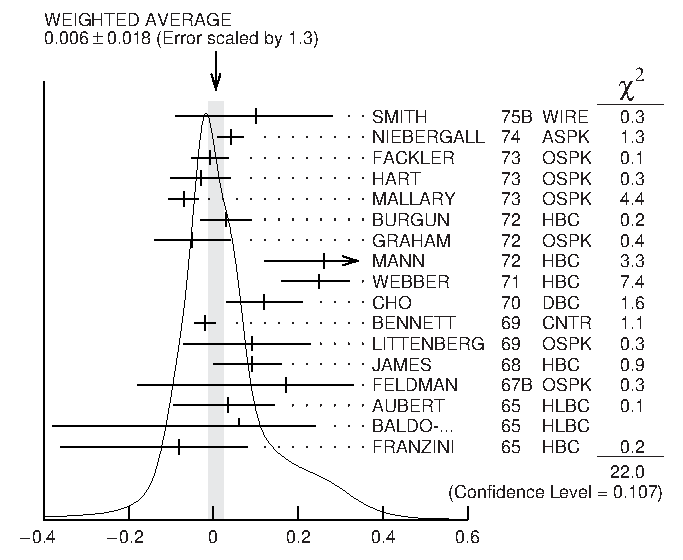
\includegraphics{filename} %multiple includegraphics may be used, 
	% with usual \hfill and \\ newline structures. 
\end{pdgxfigure}
\end{verbtex}

Figures placed in the \invt{figures} directory will be automaticallly found. 
Option keys may also be passed to individual \lstinline{\includegraphics} commands,  
as usual, if separate control is desired of multiple \lstinline{\includegraphics} in the same \invt{pdgxfigure} environment.
I.e. \lstinline!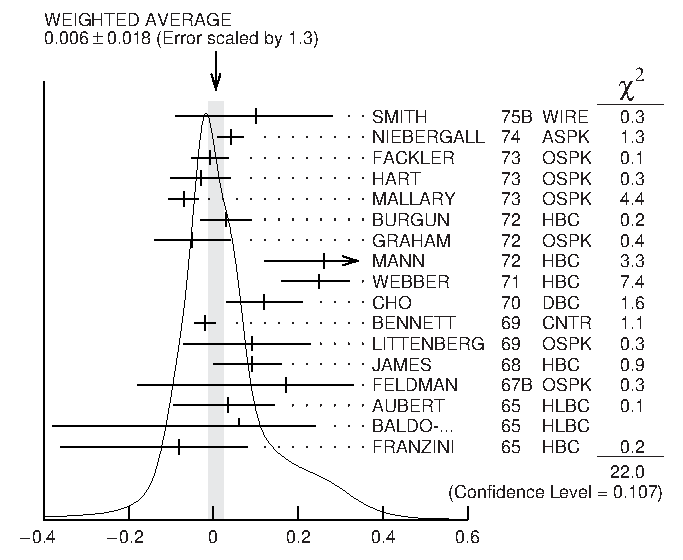
\includegraphics[<option keys>]{filename}!.

\Isubsection{Float scaling and width keys}
\label{sec:ginkeys}
As in the usual implementation of the \invt{graphicx} package, the \lstinline{\includegraphics} command takes optional standard keys \invt{width = ...}, \invt{scale = ...}.
which are used to control the width or scale of the bounding box. 
We use the same key structure to pass options to the \invt{pdgxfigure} environment, as well as to the \invt{pdgxtable} environment (see Sec.~\ref{sec:tables}).

The version specific keys \lstinline!<version>width! and \lstinline!<version>scale! have been added, 
that implement width or scaling choices only in the specific \invt{<version>}.
One may use these keys in concert with the usual \invt{width} and \invt{scale} keys, with the caveat that the order of keys matters: 
Keys are read left to right, and rightwards keys typically override leftwards ones. 
For example, passing the option keys (to either \invt{pdgxfigure} or \invt{pdgxtable}, or \lstinline{\includegraphics})
\begin{verbtex}
	[width=0.8\linewidth, bookwidth=0.9\linewidth]
\end{verbtex}
implements the \invt{width} key setting except in the book version. 
The option \lstinline!bookwidth=0.9\linewidth! followed by
\lstinline!width=0.8\linewidth! would instead implement only the version-general \lstinline!width=0.8\linewidth! setting.

\textbf{Note:} Because of specialization of the \invt{graphicx} key structure in the PDG class,
to use a \invt{scale} or \invt{<version>scale} key in an \lstinline{\includegraphics} command or \invt{pdgxfigure} environment
one must first pass an option key \invt{width=!}. This is not required for  \invt{pdgxtable}.

An additional key \lstinline!<version>bbscale! scales the float bounding box.
For some overwide floats that are larger than the nominal page width---in particular, overwide tables, see Sec.~\ref{sec:tables}---simply 
rescaling down the float does not allow it to be properly aligned on the page.
This key can be increased above $1$ (the default), to provide a sufficiently large bounding box for the float, that may then be scaled down to size with correct alignment.

\Isubsection{Available keys for \invt{pdgxfigure}}
Following is a list of available optional keys for \invt{pdgxfigure}, and default settings if not invoked.
As usual, keys are evaluated left to right. 
The version-general \invt{width} key can be used (and will override any preceeding version-specfic width key).
\begin{itemize}
	\item \invt{place}: Takes any combination of \invt{h}, \invt{t}, \invt{b}, \invt{p} (with optional \invt{\!}) that specifies float placement. Default is \invt{\!ht}.
	\item \invt{wide}: Takes \invt{true} or \invt{false} to specify the figure as full page width in either single or two column mode. Default is \invt{false}.
	\item \invt{width} or \invt{<version>width}: Sets the global or version specific width of the figure bounding box, respectively. Default is 0.75 of the line width (or text width, for wide figures).
	\item \invt{scale} or \invt{<version>scale}: Scales the figure according to float value passed to the key. 
	The option \lstinline{width=!} must be passed to turn off default width behavior and enable scaling keys.
\end{itemize}

\Isubsection{Examples}
The following produces a default-style, shown in Figure~\ref{examples:fig:example}. 
We recommend including the file extension in the \lstinline{\includegraphics} argument, to assist our editorial staff in addressing any figure quality problems.
\begin{verbtex}
\begin{pdgxfigure}[place=t] 
	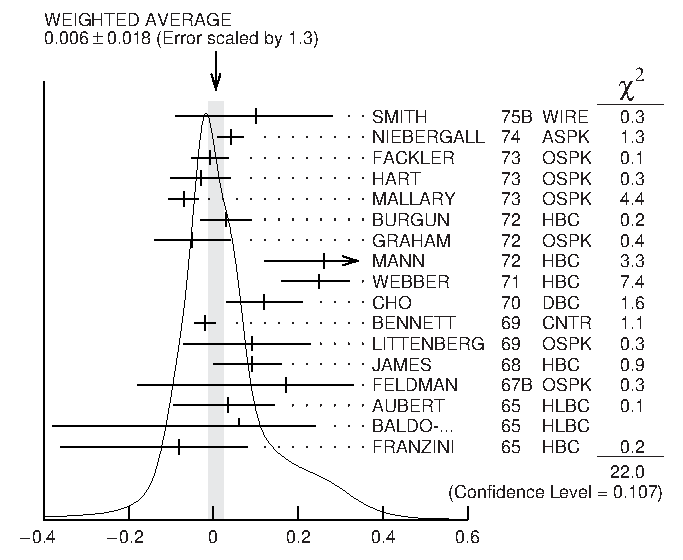
\includegraphics{filename.pdf}
	\caption{Example default figure}
	\label{examples:fig:example}
\end{pdgxfigure}
\end{verbtex}
\begin{pdgxfigure}[place=t]
	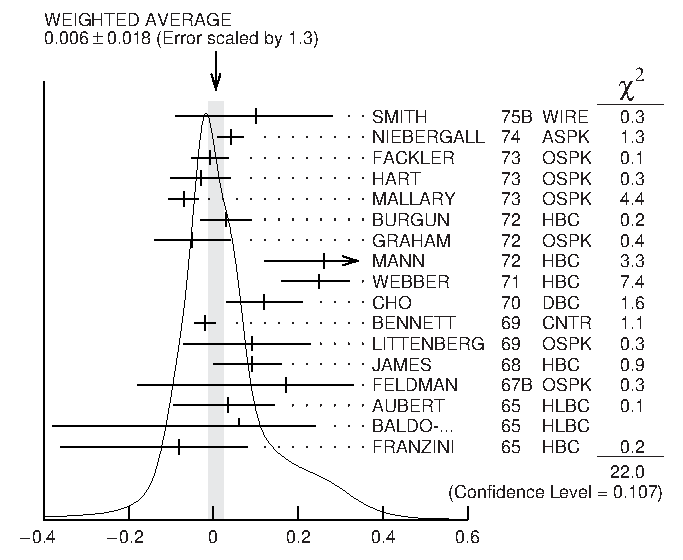
\includegraphics{filename.pdf}
	\caption{Example default figure}
	\label{examples:fig:example}
\end{pdgxfigure}

A double wide figure, shown in Fig.~\ref{examples:fig:example2}:
\begin{verbtex}
\begin{pdgxfigure}[wide=true,place=h, webwidth=0.45\linewidth, 
		bookwidth=0.9\linewidth] 
	%width key applies to all includegraphics instances
	%compiling in different versions will produce different widths
	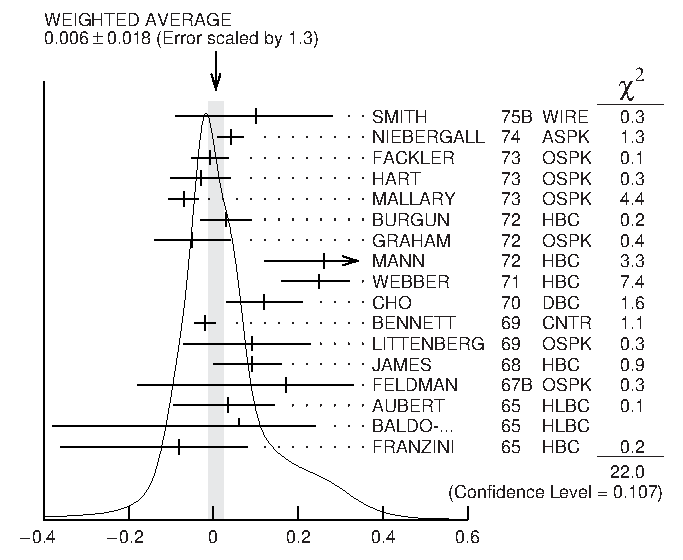
\includegraphics{filename.pdf}\hfill
	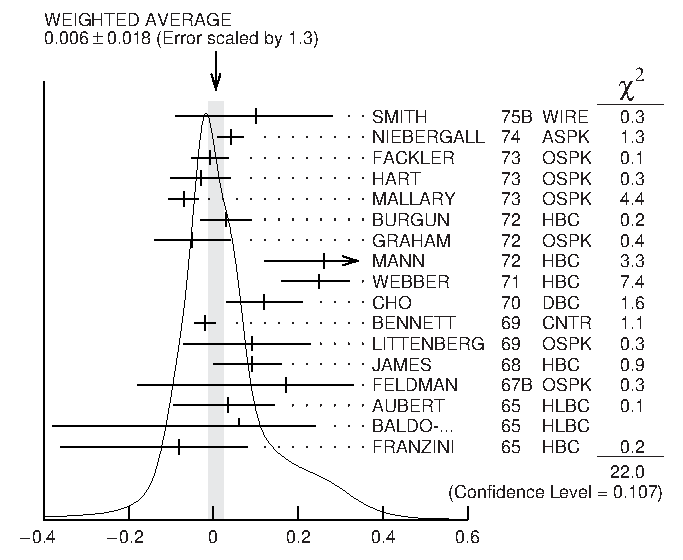
\includegraphics{filename.pdf}
	\caption{Example double wide figure, 
		with different book and web versions}
	\label{examples:fig:example2}
\end{pdgxfigure}
\end{verbtex}
\begin{pdgxfigure}[wide=true,place=h,width=0.45\textwidth] 
	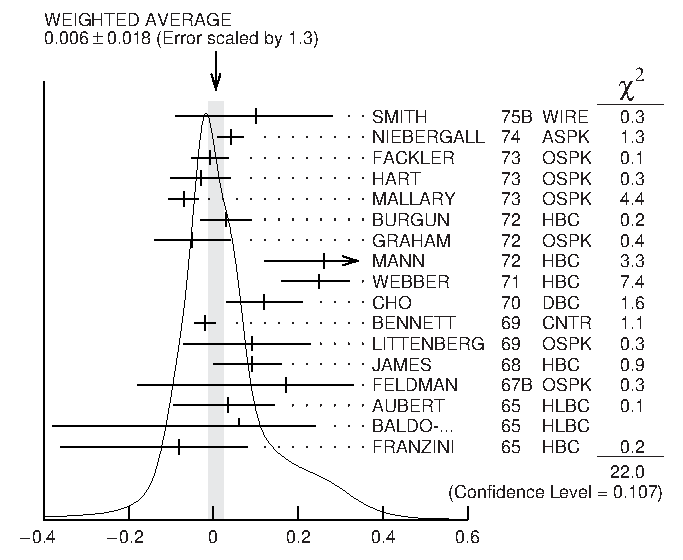
\includegraphics{filename.pdf}\hfill
	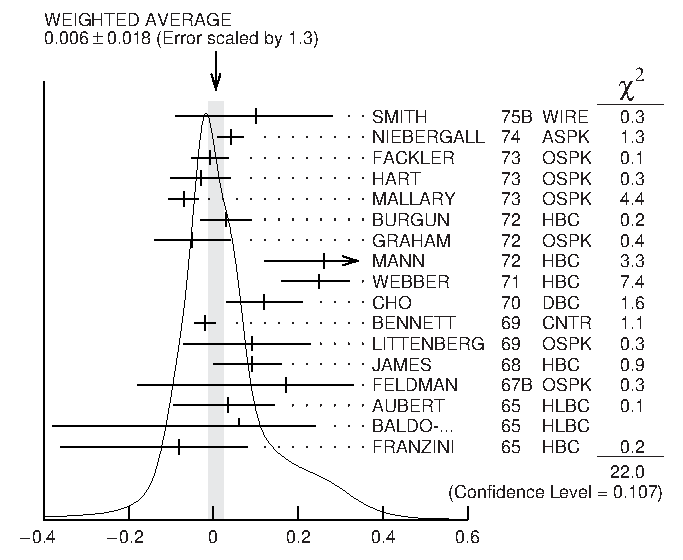
\includegraphics{filename.pdf}
	\caption{Example double wide figure, with different book and web versions}
	\label{examples:fig:example2}
\end{pdgxfigure}

A double wide figure with separate option and scaling keys, shown in Fig.~\ref{examples:fig:example3}:
\begin{verbtex}
\begin{pdgxfigure}[wide=true,place=h,width = 0.3\linewidth] 
	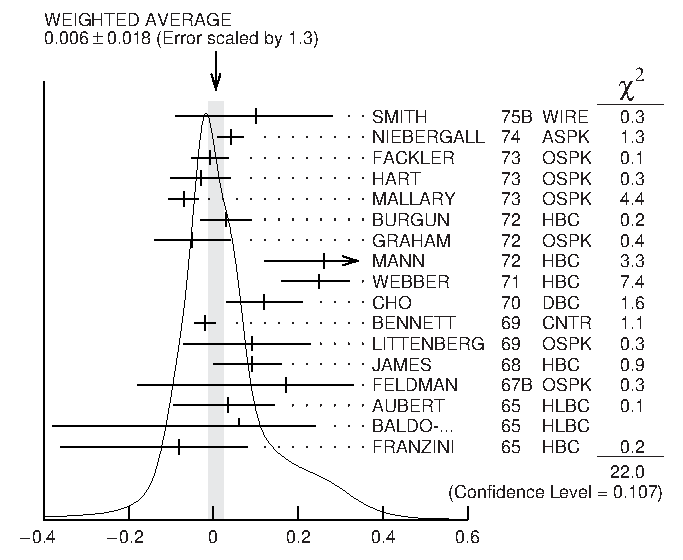
\includegraphics{filename.pdf}\hspace{1cm}
	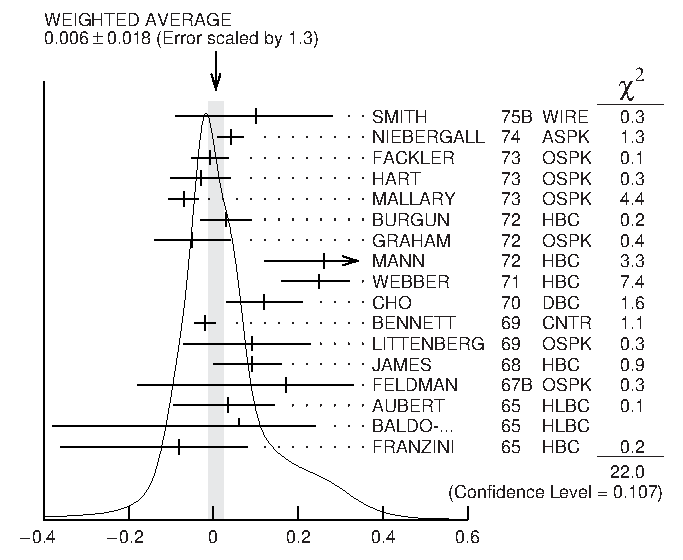
\includegraphics[width = !,scale =0.3,angle = 90]{filename}
	\caption{Example double figure, 
		with separate option and scaling keys, in both book and web versions}
	\label{examples:fig:example3}
\end{pdgxfigure}
\end{verbtex}
\begin{pdgxfigure}[wide=true,place=h,width = 0.3\linewidth] 
	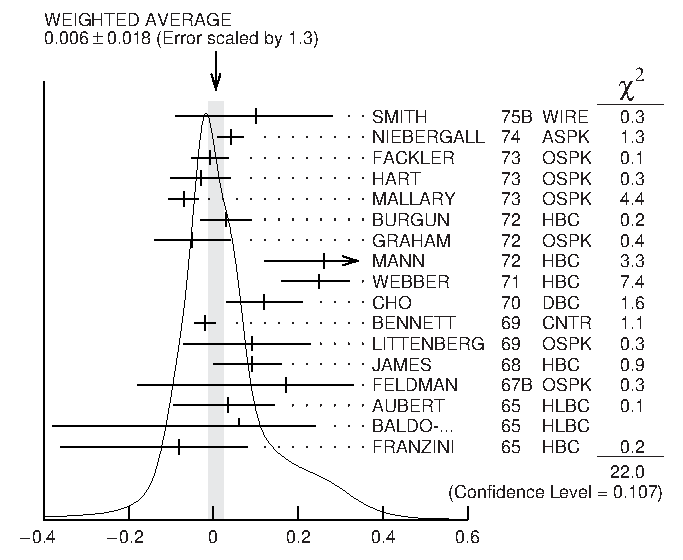
\includegraphics{filename.pdf}\hspace{1cm}
	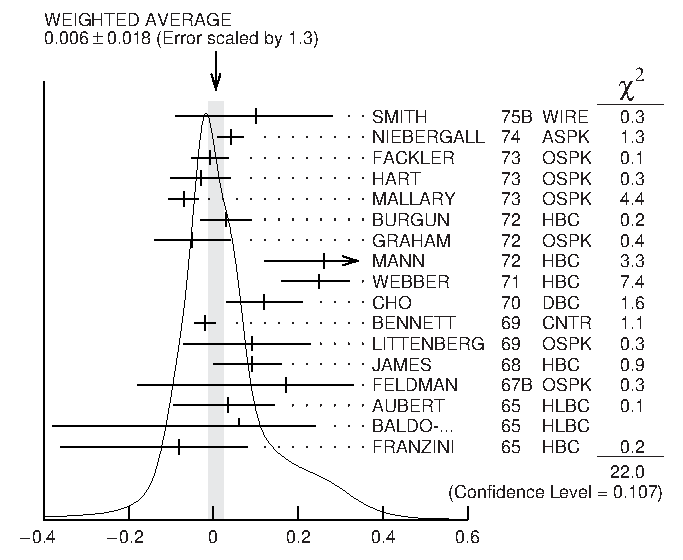
\includegraphics[width = !,scale =0.3,angle = 90]{filename}
	\caption{Example double wide figure, with separate option and scaling keys, in both book and web versions}
	\label{examples:fig:example3}
\end{pdgxfigure}

\Isubsection{\invt{pdgfigure} commands}
To add a figure, one may also use the \lstinline{\pdgfigure} or \lstinline{\pdgwidefigure} commands 
to typeset a single-column figure or double-column wide figure (for the book version), respectively. 
To include two images in one figure one may use \lstinline{\pdgdoublefigure}.
These commands are less powerful than \invt{pdgxfigure}, but automatically incorporate all PDG styles.

The macros \lstinline{\pdgfigure} and \lstinline{\pdgwidefigure} take the following arguments:
\begin{verbtex}
	\pdgfigure{<filename>}
	{<caption>}{<label>}{<placement options>}
	{<other option keys>}
\end{verbtex}
\vspace{-10pt}
while the macro \lstinline{\pdgdoublefigure} takes the following arguments:
\begin{verbtex}
	\pdgdoublefigure{<filename1>}{<filename2>}
	{<caption>}{<label>}{<placement options>}
	{<other option keys>}
\end{verbtex}
Some examples of the \invt{pdgfigure} commands are shown in Figs.~\ref{examples:fig:ideogram1}, \ref{examples:fig:ideogram2} and \ref{examples:fig:ideogram3}, respectively:
\begin{verbtex}
	\pdgfigure{filename.pdf}{Figure with caption and label}
	{examples:fig:ideogram1}{ht!}{}
	
	\pdgdoublefigure{filename.pdf}{filename.pdf}
	{Two figures, with caption and label, reduced in size}
	{examples:fig:ideogram2}{ht!}{width=0.3\textwidth}
	
	\pdgwidefigure{filename.pdf}{Wide figure}
	{examples:fig:ideogram3}{t}{}
\end{verbtex}
\FloatBarrier
\pdgfigure{filename.pdf}{Figure with caption and label}{examples:fig:ideogram1}{ht!}{}
\pdgdoublefigure{filename.pdf}{filename.pdf}{Two figures, with caption and label, reduced in size}{examples:fig:ideogram2}{ht!}{width=0.3\textwidth}
\pdgwidefigure{filename.pdf}{Wide figure}{examples:fig:ideogram3}{t}{}
\FloatBarrier

\Isection{Tables}
\label{sec:tables}
\Isubsection{ \invt{pdgxtable} and \invt{pdgxtabular}}
The PDG class provides multipurpose table and tabular environments, \invt{pdgxtable} and \invt{pdgxtabular}. 
These operate similarly to the standard \invt{table} and \invt{tabular} environments: \invt{(pdgx)table} creates a floating environment, 
while \invt{(pdgx)tabular} creates the actual tabulated display. 

The \lstinline!\caption! and \lstinline!\label! commands may be used as in the usual \invt{table} environment.
\textbf{Note: A table caption should be placed above the table.}
In addition, \invt{pdgxtable} takes a wide array of additional option keys that implement features and formatting of the prior PDG table commands/environments.  
These include keys that control placement, multicolumn spanning, version-specific widths and scaling (see Sec.~\ref{sec:ginkeys}), rotation, stretching, and caption widths.
The generic usage is
\begin{verbtex}
\begin{pdgxtable}[<option keys>]
	\caption{This is a PDG table}
	\label{tab:label}
	\begin{pdgxtabular}{<column settings>} % the usual c, l, r, | etc
		\pdgtableheader{...} %column header & separated entries go here
		%table & separated entries go here
	\end{pdgxtabular}
	%multiple pdgtabular environments are allowed
\end{pdgxtable}
\end{verbtex}

As for the usual \invt{table} environment, one may include multiple \invt{pdgxtabular}s in a single \invt{pdgxtable}.
While the \invt{pdgxtable} environment has default handling for caption widths in wide and regular tables, for both book and web versions, 
absolute control of the caption width can be implmented with a \lstinline{\captionsetup} command inside the \invt{pdgxtable} environment. 
For example \lstinline!\captionsetup{width=\linewidth}! gives a full width caption.

\Isubsection{Available keys for \invt{pdgxtable}}
Following is a list of available optional keys, and default settings if not invoked.
As usual, keys are evaluated left to right. 
While, the version-general \invt{width} key can be used (and will override any preceeding version-specfic width key), 
there is no version-general \invt{scale} key. 
Scaling of the tables is best done with the \invt{<version>scale} keys.

\begin{itemize}
	\item \invt{place}: Takes any combination of \invt{h}, \invt{t}, \invt{b}, \invt{p} (with optional \invt{\!}) that specifies float placement. Default is \invt{\!ht}.
	\item \invt{wide}: Takes \invt{true} or \invt{false} to specify the table as full page width in either single or two column mode. Default is \invt{false}.
	\item \invt{width} or \invt{<version>width}: Sets the version specific maximum width of the table bounding box. 
	Default is the maximum text width implied by the \invt{wide} key setting.
	Width settings exceeding this default are ineffective. Footnotes are scaled, but caption width is not affected.
	\item \invt{<version>scale}: Scales the table according to float value passed to the key. 
	For overwide tables, there is always a value $<1$ at which the table will be properly set to maximum page width.
	Footnotes are scaled, but caption width is not affected. Note the global \invt{scale} is disabled for \invt{pdgxtable}.
	\item \invt{<version>bbscale}: Scales the bounding box of the table. 
	For some overwide tables that are larger than the nominal page width, simply rescaling down the table does not allow the table to be properly aligned on the page.
	This key can be increased above $1$ (the default), to provide a sufficiently large bounding box for the table, that may then be scaled down to size with correct alignment.
	\item \invt{widecaptionscale}: For \invt{wide = true} tables, scales the caption width with respect to the maximum page width. Default is $0.75$.
	\item \invt{narrowcaptionscale}: For \invt{wide = false} or default tables, scales the caption width with respect to the maximum column width. Default is $0.9$.
	\item \invt{rotated}: Takes \invt{left} or \invt{right} to rotate the table, but not the caption, $90^\circ$ anticlockwise or clockwise, respectively. 
	The caption may be rotated independently, as needed with a \lstinline{\rotatebox}.
	\item \invt{sideways}: Takes \invt{true} or \invt{false} to rotate the table, including the caption, $90^\circ$ anticlockwise or clockwise, 
	according to whether the page number is even or odd.
	In a sideways table, other key width and scaling settings are still effective, but scale with respect to the page height. 
\end{itemize}


\Isubsection{Examples}
Some (simple) examples of \invt{pdgxtable} can be found in Table~\ref{examples:tab:styles} and Sec~\ref{sec:macros}.
For example, Tab.~\ref{examples:tab:styles} is typeset as
\begin{verbtex}
\begin{pdgxtable}[place=h,bookscale = 0.9,bookbbscale=2]
	\caption{Styles for the different typesetting versions}
	\label{examples:tab:styles}
	\begin{pdgxtabular}{ccccc}
		Version 		& Columns  & Font size 	& Helper Tags\footnote{
			Tags for each equation, table, figure, and bibliography entry 
			are displayed in margin or interspaced} & Line numbers\\
		\hline
		draft	& 1		   & 11pt		& Yes & Yes \\
		...
	\end{pdgxtabular}
\end{pdgxtable}
\end{verbtex}

Tables~\ref{examples:tab:commu} and~\ref{examples:tab:commp} are typeset as a two \invt{pdgxtabular}s in a single \invt{pdgxtable}, via
\begin{verbtex}
\begin{pdgxtable}[wide=true, place=!ht, webscale = 0.8]
	\caption{Common units}
	\label{examples:tab:commu}
	\begin{pdgxtabular}{lr | lr | lr}
		\showsymbol{\TeV} &  \showsymbol{\syin} & \showsymbol{\barn}   \\
		...
	\end{pdgxtabular}
	\caption{Common particles}
	\label{examples:tab:commp}
	\begin{pdgxtabular}{lr | lr | lr}
   		\showsymbol{\pp} &  \showsymbol{\ee} & \showsymbol{\pizero}   \\
  		...
	\end{pdgxtabular}
\end{pdgxtable}
\end{verbtex}

\Isubsection{Common problems and recommendations}
The \invt{pdgxtabular} environment is capable of handling the usual \lstinline{\multicolumn} and \lstinline{\multirow} objects, 
that allow for more complicated tables with cells spanning multiple rows and/or columns. 
We recommend avoiding use of \lstinline{\multispan}. 
For multiline cells, the \lstinline{\makecell} command from the \invt{makecell} package is recommended.

\Isection{Labels and referencing}
\label{sec:labels}

\Isubsection{Style guide}
As usual, the \lstinline{\label} and \lstinline{\ref} commands (and their derivatives) may be used to reference equations, tables, figures, and so on. 
To permit easy cross-referencing throughout the entire review, we request that you use the following labelling convention: \invt{BASENAME:type:name}
with \invt{type} corresponding to one of the following options
\begin{itemize}
\item {\tt fig} for figures
\item {\tt eq } for equation
\item {\tt tab} for tables
\item {\tt sec} for section, subsection etc..
\item {\tt foot} for footnotes.
\end{itemize}

\Isubsection{Missing references}

In default LaTeX, missing references are typically typeset as ``\textbf{??}''. 
To improve the typesetting experience, the \lstinline{\ref} command has been modified in the PDG class so that missing reference keys are printed out explicitly: 
For instance, a \lstinline!\ref{eqn:name}! that references a missing label called \invt{eqn:name}, will display as \ref{eqn:name}.
Similarly, the \lstinline{\cite} command will explicitly print out missing citation references. E.g. 
a \lstinline!\cite{name:2021ab}! that references a missing label called \invt{name:2021ab}, will display as \cite{name:2021ab}

\Isubsection{Cross-review referencing}
It is occasionally necessary or useful to reference (sub)sections, equations, figures, tables and so on belonging to other reviews or other reviews themselves. 
\textbf{Note:} Please use the \lstinline{\crossref} command for cross-review referencing.

Implementing a cross-reference to another review requires knowledge of its  \invt{BASENAME}:  
You must use the \invt{BASENAME} associated with the target review, not the \invt{BASENAME} of the review you're currently working on. 
To identify the  \invt{BASENAME} of another review, login into the \href{https://pdgworkspace.lbl.gov/Reviews.action}{PDG Workspace} (click to be redirected). 
Under \emph{Reviews} select from the drop-down menu \emph{All reviews}. 
Click on the title of the review you are interested in, and then select the \emph{Technical details} tab. 
The \invt{BASENAME} is the first entry.


If the full \invt{BASENAME:type:name} reference is known, you may include it with the usage \\
\lstinline!\crossref{BASENAME:type:name}!. 
This will typeset in your document as ``\crossref{BASENAME:type:name}'', because your local auxiliary files do not have the reference information of the other review.
PDG editorial staff will implement the cross-reference properly, when your review is prepared for production.

If the \invt{BASENAME:type:name} reference is not known, or the authors of the other review did not label the obect that you wish to reference, 
you may instead provide any descriptive argument to \lstinline{\crossref}. 
For example, \lstinline!\crossref{Equation 34.1.10}!.  
PDG editorial staff will implement the cross-reference properly, when your review and the other review are prepared for production.

\Isubsection{Booklet labeling and referencing}
If your review has a booklet version, it needs to be prepared at the same time as you prepare your full review.
The content to be displayed in the booklet needs to be included in \invt{BASENAME-booklet.tex}. 

The numerical tags for equations, tables, and figures in the booklet version of a review should match the tags in the full version. 
This can be achieved automatically in the booklet version by using a \lstinline!\tag{\ref{BASENAME:type:name}}! construction instead of \lstinline{\label}
to refer to the reference in the full version.
For example, if the full version has a labelled equation
\begin{verbtex}
\begin{equation}
	\label{BASENAME:eq:name}
	...
\end{equation}
\end{verbtex}
then including in \invt{BASENAME-booklet.tex}
\begin{verbtex}
\begin{equation}
	\tag{\ref{BASENAME:eq:name}}
	...
\end{equation}
\end{verbtex}
will automatically label the equation correctly. 
To achieve the same result for figures and tables, one may place in the booklet version
\begin{verbtex}
	\renewcommand{\thetable}{\ref{BASENAME:type:name}}
	\renewcommand{\thefigure}{\ref{BASENAME:type:name}}
\end{verbtex}
before each table or figure environment, respectively. 


\Isection{Index entries}
\label{sec:index}

Review authors should think about any keywords that should be included into the index of the Review of Particle Physics. PDG uses the standard \LaTeX\  \invt{makeidx} package. Thus an entry ``sample text'' can be added to the index by placing
\begin{verbtex}
\index{sample text}
\end{verbtex}
at the appropriate place in the source file. Formatting of entries with Greek letters or math symbols as well as subentries are also supported. For example
\begin{verbtex}
\index{sigma@$\$$\sigma$\$$} 
\end{verbtex}
creates an index entry $\sigma$ in the proper alphabetical order, while
\begin{verbtex}
\index{Searches!Axion searches} 
\end{verbtex}
produces a subentry ``Axion searches'' under the ``Searches'' index entry.

All index entries defined in a given review will be shown on the last page when the draft version is made. PDG staff will standardize all index entries during the final processing of all reviews. Therefore what matters is not the final formatting of index entries but that all relevant entries are added in the correct place.


\Isection{Bibliography}
\label{sec:cites}

Citations are handled using BibTeX. To add a citation to your review:
\begin{itemize}
\item Look up the reference in INSPIRE and download its BibTeX entry (see bottom of the \emph{Information} tab for the article, under \emph{Export}).
\item Add the BibTeX entry to the \invt{BASENAME.bib} file. Note the article tag assigned by INSPIRE: You can see it in the first line of the BibTeX entry, after \lstinline!@article{!.
\item Cite the reference with \lstinline{\cite}, using the article tag assigned by INSPIRE.
\end{itemize}

For example, to add a reference to the Review of Particle Physics (2018) 
add the following code to \invt{BASENAME.bib}:
\begin{verbtex}
@article{Tanabashi:2018oca,
      author         = "Tanabashi, M. and others",
      title          = "{Review of Particle Physics}",
      collaboration  = "Particle Data Group",
      journal        = "Phys. Rev.",
      volume         = "D98",
      year           = "2018",
      number         = "3",
      pages          = "030001",
      doi            = "10.1103/PhysRevD.98.030001",
      SLACcitation   = "%%CITATION = PHRVA,D98,030001;%%"
 }
\end{verbtex}
and then one may add a reference to it in \invt{BASENAME-main.tex} via \lstinline!\cite{Tanabashi:2018oca}!.

If a BibTeX entry downloaded from INSPIRE does not render correctly, 
you should first make sure you have the latest PDG style files, by running \invt{svn update} (after committing any edits you have made).
If this doesn't fix the issue please contact \invt{latexsupport@pdg.lbl.gov} for advice.  
If it appears, however, to be simply a mistake in INSPIRE's entry, 
rename the label to the form \invt{BASENAME:<INSPIRE label>} and then edit the entry as needed.
\textbf{Please do not edit entries downloaded from INSPIRE without changing the label.}
Changing the label will permit PDG editorial staff to easily identify and track edited citations, as well as notify INSPIRE of required corrections.
In case the reference does not appear in INSPIRE at all, please also use the convention for the label: \invt{BASENAME:name}.

Multiple references can be added to a single set of brackets with \lstinline!\cite{cite-key-1,cite-key-2,...}!.
One may group multiple references into the same numerical citation tag, using a \invt{*} prefix on subsequent citation keys: For example \lstinline!\cite{cite-key-1,*cite-key-2,*cite-key-3}!.
If a paper citation key is preceded by the asterisk, it can't be cited separately later, and doing so will result in a compilation error.
We recommend citing papers individually, without using the asterisk to group them.


\Isection{Footnotes}
Footnote styles are standardized throughout the review. In (rare) cases that the style needs to be changed, this is achieved via \lstinline!\setfootnotestyle{<style>}!,
where \invt{<style>} can be \lstinline{\fnsymbol} or \lstinline{\alph}, \lstinline{\Alph}, \lstinline{\arabic}, \lstinline{\roman}, \lstinline{\Roman} etc.

Sometimes the \LaTeX \ engine miscalculates the amount of space required for a footnote, resulting in overprinting of the footer.
One can help the engine obtain a better estimate by adjusting the effective page size. 
This can be done by placing \lstinline!\enlargethispage{-2\baselineskip}! somewhere just before the \lstinline{\footnote}; the \invt{-2} may be changed to any number. 

\Isection{Miscellaneous control commands}

\Isubsection{Unbalanced last page}
In the book version, the columns of the final page are automatically balanced. 
If this behavior is undesired, it may be altered by invoking \lstinline!\balancedlastpagefalse!.
The invocation may be added anywhere in the document.

\Isubsection{Blank last page}
In the book version, a blank final page may be added via \lstinline!\blankendpagetrue!.
The invocation may be added anywhere in the document.

\Isubsection{Book-only reviews}
Certain reviews are typeset for the web using the book version formatting. 
This is enforced automatically within the PDG system by \lstinline!\def\iswebbook{1}! before the \lstinline{\documentclass} invocation. 
The draft version, however, for such reviews are typeset in the usual draft/web format.

\clearpage
\Isection{PDG Macros}
\label{sec:macros}

\begin{pdgxtable}[wide=true, place=!ht, webscale = 0.8]
	\vspace{-10pt}
	\caption{Common units}
	\label{examples:tab:commu}
	\begin{pdgxtabular}{lr | lr | lr}
		\showsymbol{\TeV     } &  \showsymbol{\syin} & \showsymbol{\barn     }   \\
		\showsymbol{\MeV     } &  \showsymbol{\inch} & \showsymbol{\mbarn    }   \\
		\showsymbol{\keV     } &  \showsymbol{\ft  } & \showsymbol{\microbarn}   \\
		\showsymbol{\eV      } &  \showsymbol{\km  } & \showsymbol{\nb       }   \\
		\showsymbol{\GeVc    } &  \showsymbol{\m   } & \showsymbol{\pb       }   \\
		\showsymbol{\GeVcSq  } &  \showsymbol{\cm  } & \showsymbol{\fb       }   \\
		\showsymbol{\GeVcc   } &  \showsymbol{\mm  } & \showsymbol{\invnb    }   \\
		\showsymbol{\GeVccSq } &  \showsymbol{\mum } & \showsymbol{\invpb    }   \\
		\showsymbol{\MeVc    } &  \showsymbol{\nm  } & \showsymbol{\invfb    }   \\
		\showsymbol{\MeVcc   } &  \showsymbol{\fm  } & \showsymbol{\invab    }   \\
		\showsymbol{\invps   } &  \showsymbol{\nm  } & \showsymbol{\lum      }   \\
			&&  \showsymbol{\ma  } &&  \\
		\showsymbol{\degr    }  &  \showsymbol{\cma } && \\
			&&  \showsymbol{\mma } &&   \\
			&&  \showsymbol{\muma} &&   \\
	\end{pdgxtabular}
	\vspace{10pt}
	\caption{Common particles}
	\label{examples:tab:commp}
	\vspace{-10pt}
	\begin{pdgxtabular}{lr | lr | lr}
   \showsymbol{\pp         } &  \showsymbol{\ee           } & \showsymbol{\pizero   }   \\
   \showsymbol{\pbar       } &  \showsymbol{\epm          } & \showsymbol{\piplus   }   \\
   \showsymbol{\ppbar      } &  \showsymbol{\epem         } & \showsymbol{\piminus  }   \\
   \showsymbol{\tbar       } &  \showsymbol{\en           } & \showsymbol{\pipm     }   \\
   \showsymbol{\ttbar      } &  \showsymbol{\ep           } & \showsymbol{\pimp     }   \\
   \showsymbol{\bbar       } &  \showsymbol{\mumu         } & \showsymbol{\etaprime }   \\
   \showsymbol{\bbbar      } &  \showsymbol{\mun          } & \showsymbol{\Kzero    }   \\
   \showsymbol{\cbar       } &  \showsymbol{\mup          } & \showsymbol{\Kzerobar }   \\
   \showsymbol{\ccbar      } &  \showsymbol{\tautau       } & \showsymbol{\kaon     }   \\
   \showsymbol{\sbar       } &  \showsymbol{\taup         } & \showsymbol{\Kplus    }   \\
   \showsymbol{\ssbar      } &  \showsymbol{\taum         } & \showsymbol{\Kminus   }   \\
   \showsymbol{\ubar       } &  \showsymbol{\lepton       } & \showsymbol{\KzeroL   }   \\
   \showsymbol{\uubar      } &  \showsymbol{\leptonm      } & \showsymbol{\Kzerol   }   \\
   \showsymbol{\dbar       } &  \showsymbol{\ellm         } & \showsymbol{\Klong    }   \\
   \showsymbol{\ddbar      } &  \showsymbol{\leptonp      } & \showsymbol{\KzeroS   }   \\
   \showsymbol{\fbar       } &  \showsymbol{\ellp         } & \showsymbol{\Kzeros   }   \\
   \showsymbol{\ffbar      } &  \showsymbol{\leptonlepton } & \showsymbol{\Kshort   }   \\
   \showsymbol{\qbar       } &  \showsymbol{\ellell       } & \showsymbol{\Kstar    }   \\
   \showsymbol{\qqbar      } &  \showsymbol{\enu          } & \showsymbol{\jpsi     }   \\
   \showsymbol{\nbar       } &  \showsymbol{\munu         } & \showsymbol{\Jpsi     }   \\
   \showsymbol{\nnbar      } &  \showsymbol{\taunu        } & \showsymbol{\psip     }   \\
   \showsymbol{\neutron    } &  \showsymbol{\lnu          } & \showsymbol{\chic     }   \\
   \showsymbol{\antineutron} &  \showsymbol{\nub          } & \showsymbol{\UoneS    }   \\
   \showsymbol{\deuteron   } &  \showsymbol{\nunub        } & \showsymbol{\chib     }   \\
   \showsymbol{\Zzero      } &  \showsymbol{\nue          } & \showsymbol{\Dstar    }   \\
   \showsymbol{\Zboson     } &  \showsymbol{\nueb         } & \showsymbol{\Bd       }   \\
   \showsymbol{\Wplus      } &  \showsymbol{\nuenueb      } & \showsymbol{\Bs       }   \\
   \showsymbol{\Wminus	   } &  \showsymbol{\num          } & \showsymbol{\Bu       }   \\
   \showsymbol{\Wboson	   } &  \showsymbol{\numb         } & \showsymbol{\Bc       }   \\ 
   \showsymbol{\Wpm   	   } &  \showsymbol{\numnumb      } & \showsymbol{\Lb       }   \\
   \showsymbol{\Wmp        } &  \showsymbol{\nut          } & \showsymbol{\Bstar    }   \\
   \showsymbol{\Hzero } &  \showsymbol{\nutb         } & \showsymbol{\BoBo     }   \\
   \showsymbol{\Hboson}  &	\showsymbol{\nutnutb      } & \showsymbol{\BodBod   }    \\		    
   \showsymbol{            } &	\showsymbol{              } & \showsymbol{\BosBos   }    \\		    
   \showsymbol{            } &	\showsymbol{              } & \showsymbol{\LambdaStar}  \\
	\end{pdgxtabular}
\end{pdgxtable}

\begin{pdgxtable}[wide=true, place=h, webscale = 0.8]
	\caption{Hypothetical particles}
	\begin{pdgxtabular}{lr | lr | lr}
   \showsymbol{\Azero }      &  \showsymbol{\gravino   } & \showsymbol{\slepton   }   \\
   \showsymbol{\hzero }      &  \showsymbol{\Zprime    } & \showsymbol{\sleptonL  }   \\
   \showsymbol{\Hzero }      &  \showsymbol{\Zstar     } & \showsymbol{\sleptonR  }   \\
   \showsymbol{\Hplus }  	  &  \showsymbol{\squark    } & \showsymbol{\sel       }   \\
   \showsymbol{\Hminus}       &  \showsymbol{\squarkL   } & \showsymbol{\selL      }   \\
   \showsymbol{\Hpm   }   	&  \showsymbol{\squarkR   } & \showsymbol{\selR      }   \\
   \showsymbol{\Hmp   }       &  \showsymbol{\gluino    } & \showsymbol{\smu       }   \\
   \showsymbol{\ggino }     &  \showsymbol{\stop      } & \showsymbol{\smuL      }   \\
   \showsymbol{\chinop}      &  \showsymbol{\stopone   } & \showsymbol{\smuR      }   \\
   \showsymbol{\chinom}      &  \showsymbol{\stoptwo   } & \showsymbol{\stau      }   \\
   \showsymbol{\chinopm}      &  \showsymbol{\stopL     } & \showsymbol{\stauL     }   \\
   \showsymbol{\chinomp}     &  \showsymbol{\stopR     } & \showsymbol{\stauR     }   \\
   \showsymbol{\chinoonep}     &  \showsymbol{\sbottom   } & \showsymbol{\stauone   }   \\
   \showsymbol{\chinoonem}   &  \showsymbol{\sbottomone} & \showsymbol{\stautwo   }   \\
   \showsymbol{\chinoonepm}   &  \showsymbol{\sbottomtwo} & \showsymbol{\snu       }   \\
   \showsymbol{\chinotwop}  &  \showsymbol{\sbottomL  } & \showsymbol{           }   \\
   \showsymbol{\chinotwom}   &  \showsymbol{\sbottomR  } & \showsymbol{           }   \\
   \showsymbol{\chinotwopm}   &  \showsymbol{           } & \showsymbol{           }   \\
   \showsymbol{\nino}  &  \showsymbol{           } & \showsymbol{           }   \\
   \showsymbol{\ninoone}        &  \showsymbol{           } & \showsymbol{           }   \\
   \showsymbol{\ninotwo}     &  \showsymbol{           } & \showsymbol{           }   \\
   \showsymbol{\ninothree}     &  \showsymbol{           } & \showsymbol{           }   \\
   \showsymbol{\ninofour}   &  \showsymbol{           } & \showsymbol{           }   \\
	\end{pdgxtabular}
\vspace*{10pt}
	\caption{Useful symbols for proton-proton physics}
\vspace*{-10pt}	
	\begin{pdgxtabular}{lr | lr }
   \showsymbol{\pT  }      &  \showsymbol{\rts }   \\
   \showsymbol{\pt  }      &  \showsymbol{\sqs } \\
   \showsymbol{\ET  }      &  \showsymbol{\mh}  \\
   \showsymbol{\eT  }      &  \showsymbol{\mW}  \\
   \showsymbol{\et  }      & \showsymbol{\mZ}   \\
   \showsymbol{\HT  }      & \showsymbol{\mH}   \\
   \showsymbol{\pTsq}      &&   \\
   \showsymbol{\MET }      &&   \\
   \showsymbol{\met }      &&   \\
   \showsymbol{\Ecm }      &&   \\
	\end{pdgxtabular}
\vspace*{10pt}
	\caption{Monte Carlo Generators}
\vspace*{-10pt}		
	\begin{pdgxtabular}{lr | lr | lr}	
   \showsymbol{\ACERMC    }      &  \showsymbol{\MCatNLO   } & \showsymbol{\Comphep    }   \\
   \showsymbol{\ALPGEN    }      &  \showsymbol{\AMCatNLO  } & \showsymbol{\Prospino   }   \\
   \showsymbol{\GEANT     }      &  \showsymbol{\MCFM      } & \showsymbol{\LO         }   \\
   \showsymbol{\Herwigpp  }      &  \showsymbol{\METOP     } & \showsymbol{\NLO        }   \\
   \showsymbol{\HERWIGpp  }      &  \showsymbol{\POWHEG    } & \showsymbol{\NLL        }   \\
   \showsymbol{\Herwig    }      &  \showsymbol{\POWHEGBOX } & \showsymbol{\NNLO       }   \\
   \showsymbol{\HERWIG    }      &  \showsymbol{\POWPYTHIA } & \showsymbol{\muF        }   \\
   \showsymbol{\JIMMY     }      &  \showsymbol{\PROTOS    } & \showsymbol{\muR        }   \\
   \showsymbol{\MADSPIN   }      &  \showsymbol{\PYTHIA    } & \showsymbol{            }   \\
   \showsymbol{\MADGRAPH  }      &  \showsymbol{\SHERPA    } & \showsymbol{            }   \\
   \showsymbol{\MGMCatNLO }      &  \showsymbol{           } & \showsymbol{            }   \\
	\end{pdgxtabular}
\end{pdgxtable}

\Isection{Tables: Legacy commands}

Though no longer recommended, legacy \lstinline{\pdgtable} or \lstinline{\pdgwidetable} commands 
to typeset a single-column table or double-column wide table (for the book version), respectively.
The \lstinline{\pdgtableheader} macro may be used in the first line of the table to automatically typeset a header.

The macros \lstinline{\pdgtable} and \lstinline{\pdgwidetable} take the following arguments:
\begin{verbtex}
	\pdgtable{<column styles>}
	{<caption>}{<label>}{<option keys>}
\end{verbtex}
Some examples usages of these commands follow, in Tables~\ref{examples:tab:table1}, \ref{examples:tab:table2} and~\ref{examples:tab:table3} below.
\begin{verbtex}
\begin{pdgtable}{c c c} 
	{Table}{examples:tab:table1}{h!}
	\pdgtableheader{ Column 1 & Column 2 & Column 3}
	row1  & 1  & 2\\
	row2  & 1  & 2\\
	row3  & 1  & 2\\
\end{pdgtable}
\end{verbtex}   
\begin{verbtex}
\begin{pdgtable}{|c | c | c | c|} 
	{Multicolumn table}{examples:tab:table2}{h!}
	\pdgtableheader{ \multicolumn{2}{c}{Column 1} & 
	\multicolumn{2}{c}{Column 2}}
	\pdgtableheader{ A & B& C & D }
	row1  & 1 & 2 &3 \\
	row2  & 1 & 2 &3 \\
\end{pdgtable}
\end{verbtex}  
\begin{verbtex}
\begin{pdgtable}{c l}
	{Table with footnotes}{examples:tab:table3}{}
	One value & another\footnote{This is something to notice
	\label{kmmix:foot:one}}\\
	Two values\footref{kmmix:foot:one} & another \\
\end{pdgtable}
\end{verbtex} 
 
\FloatBarrier 
\begin{pdgtable}{c c c} 
{Table}{examples:tab:table1}{h!}
\pdgtableheader{ Column 1 & Column 2 & Column 3}
row1  & 1  & 2\\
row2  & 1  & 2\\
row3  & 1  & 2\\
\end{pdgtable}
\begin{pdgtable}{|c | c | c | c|} 
{Multicolumn table}{examples:tab:table2}{h!}
\pdgtableheader{ \multicolumn{2}{|c|}{Column 1} & 
\multicolumn{2}{|c|}{Column 2}}
\pdgtableheader{ A & B& C & D }
row1  & 1 & 2 &3 \\
row2  & 1 & 2 &3 \\
\end{pdgtable}
\begin{pdgtable}{c l}
{Table with footnotes}{examples:tab:table3}{}
One value & another\footnote{This is something to notice\label{kmmix:foot:one}}\\
Two values\footref{kmmix:foot:one} & another \\
\end{pdgtable}
! line that includes these instructions in the main source file of your review, \invt{databases-main.tex}.

This documentation focuses mostly on the specialized functionality of the PDG \LaTeX \ class: %There are many resources that provide more general guidance for typesetting in \LaTeX.
For further support, or any \LaTeX-related questions, we invite authors to contact
\vspace{-0.2cm}
\begin{center}
\scalebox{1.5}{
	\invt{latexsupport@pdg.lbl.gov}
}
\end{center}

\Isubsection{File structure}
The source files for a PDG review are kept in separate directories within a SVN repository. 
Some files in each directory are auto-generated, while others are designed to be edited by review authors. 
\textbf{Do not edit auto-generated files, as any edits to these files will be overwritten periodically.}

Each review is assigned a unique name ("basename") that is used to label the relevant review files and will be referred to as \invt{BASENAME} in the following. For example, the QCD review is assigned basename \invt{qcd}. Therefore \invt{BASENAME-main.tex} in this documentation refers to file \invt{qcd-main.tex} for the QCD review.

Your review is assigned basename \invt{databases}.

The basename is further used to label cross-references to the review (see Sec.~\ref{sec:labels}) and specialized citations (see Sec.~\ref{sec:cites}). 
The file structure of a typical review is as follows:
\begin{itemize}
\item \invt{BASENAME-main.tex} --- contains the text of your review. 
\item \invt{BASENAME-booklet.tex} --- contains the text of the booklet version of your review (if there is one)
\item \invt{BASENAME-preamble.tex} --- contains review-specific definitions or inclusion of packages, that need to go into the document's preamble
\item \invt{BASENAME.bib} --- BibTeX bibliography entries (see Sec~\ref{sec:cites})
\item \invt{/figures} --- directory containing all figures
\item Auxiliary files (\invt{.aux}, \invt{.out}, \invt{.log}) --- these are generated by the \LaTeX compiler
\item Other \invt{.tex} files --- may be added and included in \invt{BASENAME-main.tex} or \invt{BASENAME-booklet.tex} with the \lstinline{\input} command.
\item \textbf{[auto-generated]} \invt{BASENAME.tex} --- compilation file for the review
\item \textbf{[auto-generated]} \invt{Makefile} --- Makefile to compile the review automatically (see Sec.~\ref{sec:make})
\item \textbf{[auto-generated]} \invt{pdg.cls} --- PDG \LaTeX \ class file
\item \textbf{[auto-generated]} \invt{pdg.bst} --- BibTeX PDG style file
\item \textbf{[auto-generated]} \invt{pdg-xr-hyper.sty} --- helper BibTeX style file
\item \textbf{[auto-generated]} \invt{pdgdefs.tex} --- PDG standard symbols and macros
\item \textbf{[auto-generated]} \invt{examples.tex} --- This file
\end{itemize}

\begin{center}
~\\
%!%\vspace{-12pt}
%!%In your review, the basename is databases.
\end{center}
To identify the  \invt{BASENAME} of yours or another review, you may also login into the 
\href{https://pdgworkspace.lbl.gov/Reviews.action}{PDG Workspace} (click to be redirected). 
Under \emph{Reviews} select from the drop-down menu \emph{All reviews}. 
Click on the title of the review you are interested in, and then select the \emph{Technical details} tab. 
The \invt{BASENAME} is the first entry.

\Isubsection{Multiversion typesetting}
The PDG \LaTeX \ class has functionality to typeset in four different versions or styles: draft, web, book and booklet. 
(The draft and web versions are referred to below jointly as `web', since they are broadly similar). 
See Table~\ref{examples:tab:styles} for a broad summary.

\begin{pdgxtable}[place=h,bookscale = 0.9,bookbbscale=2]
	\caption{Styles for the different typesetting versions}
	\label{examples:tab:styles}
	\begin{pdgxtabular}{ccccc}
		Version 		& Columns  & Font size 	& Helper Tags\footnote{
			Tags for each equation, table, figure, and bibliography entry are displayed in margin or interspaced} & Line numbers\\
		\hline
		\invt{draft} 	& 1		   & 11pt		& Yes & Yes \\
		\invt{web} 		& 1		   & 11pt		& No  & No\\
		\invt{book} 	& 2		   & 8pt		& No  & No\\
		\invt{booklet} 	& 1		   & 8pt		& No & No \\
	\end{pdgxtabular}
\end{pdgxtable}

Specialized macros may also have version-specific implementations. 
These follow the naming convention \invt{<version><macroname>}, where \invt{<version>} may take values of \invt{book}, \invt{booklet} and \invt{web}.
See for example, Sec.~\ref{sec:align}.
Specialized option keys follow the same convention. See e.g. Sec.~\ref{sec:ginkeys}.


\Isubsection{Makefile}
\label{sec:make}
We recommend to compile the review using \invt{make} on the command line. The usage is as follows:
\begin{itemize}
	\item \invt{make} --- compiles in draft mode.
	\item \invt{make  <version>} --- compiles in \invt{<version>} mode. For example \invt{make web}.
	\item \invt{make bib} --- compiles only the BibTeX files.
	\item \invt{make clean} --- cleans out all auxiliary files.
	\item \invt{make cleanall} --- cleans out the compiled pdf and all auxiliary files.
	\item \invt{make prod} --- cleans all auxiliary files, then compiles the web version.
	\item {\footnotesize{\texttt{make crossref}}} --- compiles required cross-referencing files (advanced: requires checkout of the other reviews to be cross-referenced).
\end{itemize}



\Isection{Style guides}
\Isubsection{Particle symbols}
Particle symbols are italic (or slanted) characters: \en, \pbar, \Lb, \pizero, \Klong, \Dstar. 
Charge is indicated by a superscript: $B^{-}$, $\Delta^{++}$. 
Charge is not normally indicated for $p$, $n$, or the quarks, and is optional for neutral isosinglets: $\eta$ or $\eta^{0}$. 
Antiparticles and particles are distinguished by charge for
charged leptons and mesons: $\tau^{+}$, $\kaon^{-}$ 
Otherwise, distinct antiparticles are indicated by a bar (overline): $\nbar_{\mu}$, \tbar, \pbar, \Kzerobar.

\Isubsection{Macros and shortcuts}
The \invt{pdgdefs.tex} file implements a series of useful macros for particle symbols, units and other common notation. 
All definitions are terminated with  \lstinline!\string\xspace!, so you can simply write ``\lstinline!\ttbar production!'' to typeset inline ``\ttbar production''.
The entire list of macros is provided in Sec.~\ref{sec:macros}.

Most Monte Carlo generators have a macro with a suffix 'V' that allows you to include the version. E.g. \lstinline!\PYTHIAV{8.1}! produces \PYTHIAV{8.1}.
In case you need to define other symbols, please add them to the \invt{BASENAME-preamble.tex} file.

\Isubsection{Column switching}

The web version is typeset as single column, singleside 11pt style, the book as 8pt double column, double sided.

In all versions of the review, switching between single and double column mode can be done \emph{in situ} with \lstinline{\onecolumn} or \lstinline{\twocolumn}
respectively. For example

\medskip
\ifrppbook
	\onecolumn
\else
	\twocolumn
\fi
{\footnotesize{Lorem ipsum dolor sit amet, consectetur adipiscing elit. Duis congue lectus at lectus tristique porta. Vivamus scelerisque porta massa, laoreet pulvinar dolor blandit vitae. Nam rhoncus id risus in tincidunt. Maecenas ultrices, arcu id gravida tempor, urna libero sodales nunc, quis dapibus ipsum quam eget est. Quisque eget convallis odio, at pellentesque quam. Mauris pretium eu metus ac imperdiet. Class aptent taciti sociosqu ad litora torquent per conubia nostra, per inceptos himenaeos. Nulla quis tincidunt libero. Aliquam posuere at quam quis posuere. Etiam turpis nulla, faucibus eget massa sagittis, porttitor sagittis elit. Proin a lorem eleifend, rhoncus orci quis, mattis metus. Donec sit amet lobortis lacus. Quisque magna augue, elementum nec ipsum non, feugiat ultricies urna. Sed tincidunt nisl vestibulum leo finibus, vitae sollicitudin sapien bibendum. Duis maximus ipsum nec urna lobortis, sed scelerisque nulla facilisis. Sed id finibus libero. }}
\ifrppbook
	\twocolumn
\else
	\onecolumn
\fi
\medskip

\Isection{Equations}
Equations may be typeset using the \invt{equation}, \invt{array}, \invt{multline}, and \invt{gather} etc environments provided by \invt{amsmath} package. 
We do not recommend using \invt{eqnarray}. As a trivial example
\begin{verbtex}
\begin{equation}
\label{BASENAME:eq:equation}
	N_{exp} = \sigma_{exp} \times \int L(t) dt
\end{equation}
\end{verbtex}
which produces
\begin{equation}
	N_{exp} = \sigma_{exp} \times \int L(t) dt
\end{equation}


To tag a set of equations with a common numbering and label, please use the \invt{subequation} environment, together with \invt{align}.
As an example:
\begin{verbtex}
\begin{subequations}
	\label{BASENAME:eq:equation1}
	\begin{align}
		A + B = C\\
		D= \frac{E}{F}  
	\end{align}
\end{subequations}
\end{verbtex}
which produces
\begin{subequations}
\begin{align}
	A + B = C\\
	D= \frac{E}{F}  
\end{align}
\end{subequations}


\Isubsection{Wide equations: \invt{pdgstrip}}
Some wide equations are not easily amenable to display in the PDG book double column format. 
Similar to the ReVTeX \invt{widetext} environment, the PDG style provides a \invt{pdgstrip} environment, that may wrap any other equation (or align, array etc) environment. 
The \invt{pdgstrip} environment is not a float, and will respect absolute placement in the typesetting stream. 
For example:
\begin{verbtex}
	\begin{pdgstrip}
		\begin{equation} % or any other display environment
		...

		\end{equation}
	\end{pdgstrip}
\end{verbtex}
In the web and booklet versions, this environment performs no operation on the wrapped environment. 
In the book version, the equation is preserved as a single `strip' across both columns, with column-wide rules to guide the reader's eye. 
The column-wide rules may be disabled -- e.g if the strip environment falls at the top or bottom of a page --  by passing the option \invt{plain} to the \invt{pdgstrip} environment. I.e. 
\lstinline!\begin{pdgstrip}[plain]!.

In principle, the pdgstrip envirornment may also wrap a floating environment such as a figure. 
In the book version, this will disable the ability of the figure to float, and fix it to a desired location.

\Isubsection{Alignment}
\label{sec:align}
Within \invt{align} environments or any other environment that uses the special \invt{&} and \invt{\\\\} (or \lstinline{\cr}) control characters for alignment, one may use
use version specific \lstinline!\bookalign!, \lstinline!\webalign!, \lstinline!\bookletalign! and \lstinline!\bookcr!, \lstinline!\webcr!, \lstinline!\bookletcr! macros.

The \lstinline!\<version>align! macros insert a `\invt{&}' control character only in the \invt{<version>} of the review. 
The \lstinline!\<version>cr! macro similarly inserts a carriage return `\invt{\\\\}' only in the \invt{<version>} of the review, 
but takes two additional arguments that are placed before and after the carriage return, respectively. For instance,
\lstinline!\bookcr{\nonumber}{[10pt]}! inserts \lstinline!\nonumber\\[10pt]!.  An example usage is
\begin{verbtex}
\begin{align}
	{\cal A}_f 
	\bookalign = \frac{\Gamma(\bar{B}^0(t) \to f) - \Gamma(B^0(t) \to f)}
		{\Gamma(\bar{B}^0(t) \to f) + \Gamma(B^0(t) \to f)} \bookcr{\,,\nonumber}{}
	\bookalign = S_f \sin(\Delta m_d\, t) - C_f \cos(\Delta m_d\, t) \,.
\end{align}
\end{verbtex}
This produces in the web version
\ifrppbook
\onecolumn
	\begin{align}
		{\cal A}_f  = \frac{ \Gamma(\bar{B}^0(t) \to f) - \Gamma(B^0(t) \to  f) }
			{ \Gamma(\bar{B}^0(t) \to f) + \Gamma(B^0(t) \to  f) } 
			= S_f \sin(\Delta m_d\, t) - C_f \cos(\Delta m_d\, t) \,,
	\end{align}
\twocolumn
\else
	\begin{align}
		{\cal A}_f 
		\bookalign = \frac{ \Gamma(\bar{B}^0(t) \to f) - \Gamma(B^0(t) \to  f) }
			{ \Gamma(\bar{B}^0(t) \to f) + \Gamma(B^0(t) \to  f) } \bookcr{\,,\nonumber}{}
		\bookalign = S_f \sin(\Delta m_d\, t) - C_f \cos(\Delta m_d\, t) \,,
	\end{align}
\fi	
and in the two column book version
\addtocounter{equation}{-1}
\ifrppweb
	\twocolumn
	\begin{align}
		{\cal A}_f 
		& = \frac{ \Gamma(\bar{B}^0(t) \to f) - \Gamma(B^0(t) \to  f) }
			{ \Gamma(\bar{B}^0(t) \to f) + \Gamma(B^0(t) \to  f) } \,,\nonumber\\
		& = S_f \sin(\Delta m_d\, t) - C_f \cos(\Delta m_d\, t) \,,
	\end{align}
	\onecolumn
\else
	\begin{align}
		{\cal A}_f 
		\bookalign = \frac{ \Gamma(\bar{B}^0(t) \to f) - \Gamma(B^0(t) \to  f) }
			{ \Gamma(\bar{B}^0(t) \to f) + \Gamma(B^0(t) \to  f) } \bookcr{\,,\nonumber}{}
		\bookalign = S_f \sin(\Delta m_d\, t) - C_f \cos(\Delta m_d\, t) \,,
	\end{align}
\fi

\Isection{Figures}

\Isubsection{Figure requirements}
Permitted figure formats (for pdflatex) are pdf, png and jpg, in order of preferred format. 
In addition, please note:
\begin{itemize}
	\item Submissions should be be provided with a minimum resolution of 150DPI. However, 300DPI or greater is preferred.
	\item Our preference for the submission color palette is CMYK, but RGB is acceptable.
	\item Visible line (stroke) weight must be no less than $0.5$px, preferably at least $1$px.
	\item Submissions should be provided with fonts embedded, if possible.
	\item In print, colors are often not as vibrant or saturated as they appear on screen. Therefore, overlapping areas of color should be high contrast for visual clarity: 
	e.g. do not place magenta over blue, or light blue over a light green.	
\end{itemize}
If you are unsure your figure is of sufficient resolution or quality, please contact \invt{latexsupport@pdg.lbl.gov} for advice.

Encapsulated postscript or postscript figures may also be used, but they require conversion to pdf. 
Depending on your \LaTeX \ engine settings, running \invt{pdflatex} may automatically convert eps or ps files. 
If not, the conversion can be done manually with various programs, such as ImageMagick, or \invt{epstopdf} and \invt{pstopdf}.

\textbf{Note:} Make sure that the figure file is added into the subdirectory \invt{figures}, and that it is commited to svn or provided with your text.

\Isubsection{\invt{pdgxfigure} environment}
The multipurpose figure environment \invt{pdgxfigure} is now available, as an alternative to the various \invt{pdgfigure} and related commands.
These operate similarly to the standard \invt{figure} environments: \invt{(pdgx)figure} creates a floating environment.

The \lstinline!\caption! and \lstinline!\label! commands may be used as in the usual \invt{figure} environment. 
\textbf{Note: A figure caption should be placed below the figure.}
In addition, \invt{pdgxfigure} takes an array of additional option keys that implement features and formatting of the prior PDG figure commands.
These include keys that control placement, multicolumn spanning, and version-specific widths. 
The generic usage is
\begin{verbtex}
\begin{pdgxfigure}[<option keys>]
	\caption{This is a PDG figure}
	\label{examples:fig:label}
	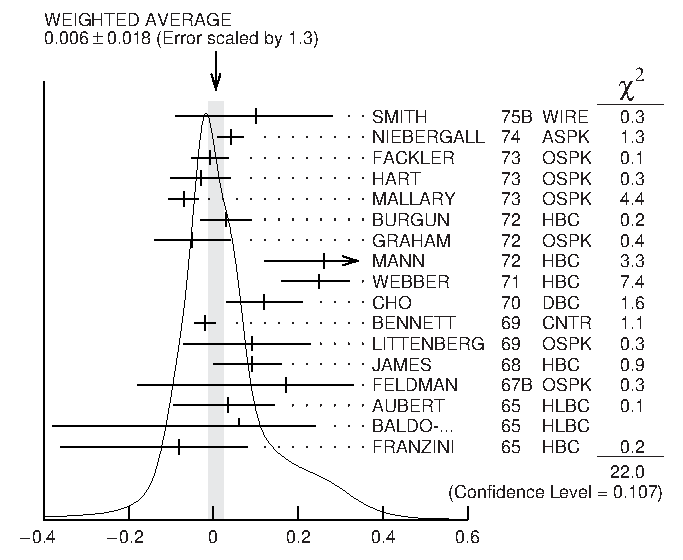
\includegraphics{filename} %multiple includegraphics may be used, 
	% with usual \hfill and \\ newline structures. 
\end{pdgxfigure}
\end{verbtex}

Figures placed in the \invt{figures} directory will be automaticallly found. 
Option keys may also be passed to individual \lstinline{\includegraphics} commands,  
as usual, if separate control is desired of multiple \lstinline{\includegraphics} in the same \invt{pdgxfigure} environment.
I.e. \lstinline!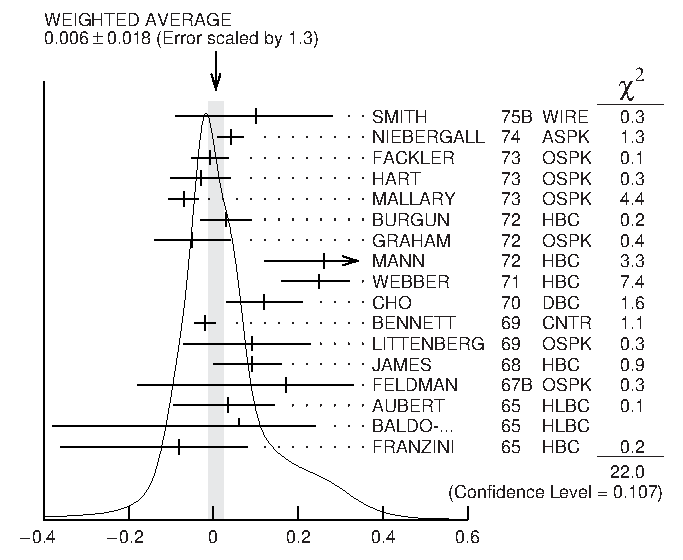
\includegraphics[<option keys>]{filename}!.

\Isubsection{Float scaling and width keys}
\label{sec:ginkeys}
As in the usual implementation of the \invt{graphicx} package, the \lstinline{\includegraphics} command takes optional standard keys \invt{width = ...}, \invt{scale = ...}.
which are used to control the width or scale of the bounding box. 
We use the same key structure to pass options to the \invt{pdgxfigure} environment, as well as to the \invt{pdgxtable} environment (see Sec.~\ref{sec:tables}).

The version specific keys \lstinline!<version>width! and \lstinline!<version>scale! have been added, 
that implement width or scaling choices only in the specific \invt{<version>}.
One may use these keys in concert with the usual \invt{width} and \invt{scale} keys, with the caveat that the order of keys matters: 
Keys are read left to right, and rightwards keys typically override leftwards ones. 
For example, passing the option keys (to either \invt{pdgxfigure} or \invt{pdgxtable}, or \lstinline{\includegraphics})
\begin{verbtex}
	[width=0.8\linewidth, bookwidth=0.9\linewidth]
\end{verbtex}
implements the \invt{width} key setting except in the book version. 
The option \lstinline!bookwidth=0.9\linewidth! followed by
\lstinline!width=0.8\linewidth! would instead implement only the version-general \lstinline!width=0.8\linewidth! setting.

\textbf{Note:} Because of specialization of the \invt{graphicx} key structure in the PDG class,
to use a \invt{scale} or \invt{<version>scale} key in an \lstinline{\includegraphics} command or \invt{pdgxfigure} environment
one must first pass an option key \invt{width=!}. This is not required for  \invt{pdgxtable}.

An additional key \lstinline!<version>bbscale! scales the float bounding box.
For some overwide floats that are larger than the nominal page width---in particular, overwide tables, see Sec.~\ref{sec:tables}---simply 
rescaling down the float does not allow it to be properly aligned on the page.
This key can be increased above $1$ (the default), to provide a sufficiently large bounding box for the float, that may then be scaled down to size with correct alignment.

\Isubsection{Available keys for \invt{pdgxfigure}}
Following is a list of available optional keys for \invt{pdgxfigure}, and default settings if not invoked.
As usual, keys are evaluated left to right. 
The version-general \invt{width} key can be used (and will override any preceeding version-specfic width key).
\begin{itemize}
	\item \invt{place}: Takes any combination of \invt{h}, \invt{t}, \invt{b}, \invt{p} (with optional \invt{\!}) that specifies float placement. Default is \invt{\!ht}.
	\item \invt{wide}: Takes \invt{true} or \invt{false} to specify the figure as full page width in either single or two column mode. Default is \invt{false}.
	\item \invt{width} or \invt{<version>width}: Sets the global or version specific width of the figure bounding box, respectively. Default is 0.75 of the line width (or text width, for wide figures).
	\item \invt{scale} or \invt{<version>scale}: Scales the figure according to float value passed to the key. 
	The option \lstinline{width=!} must be passed to turn off default width behavior and enable scaling keys.
\end{itemize}

\Isubsection{Examples}
The following produces a default-style, shown in Figure~\ref{examples:fig:example}. 
We recommend including the file extension in the \lstinline{\includegraphics} argument, to assist our editorial staff in addressing any figure quality problems.
\begin{verbtex}
\begin{pdgxfigure}[place=t] 
	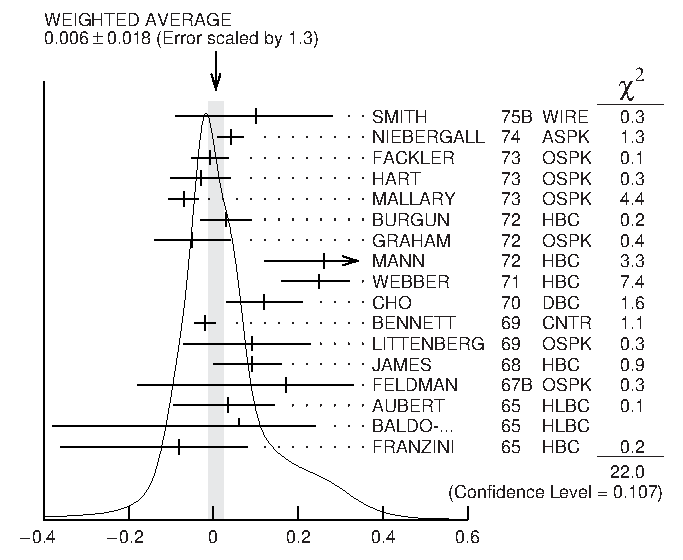
\includegraphics{filename.pdf}
	\caption{Example default figure}
	\label{examples:fig:example}
\end{pdgxfigure}
\end{verbtex}
\begin{pdgxfigure}[place=t]
	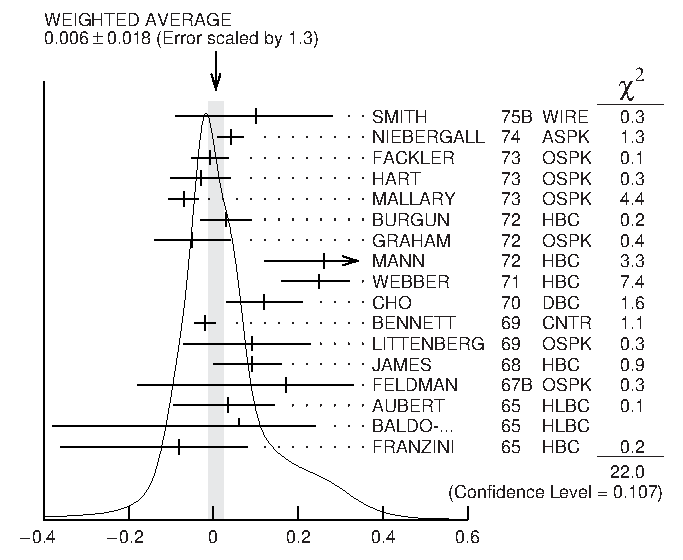
\includegraphics{filename.pdf}
	\caption{Example default figure}
	\label{examples:fig:example}
\end{pdgxfigure}

A double wide figure, shown in Fig.~\ref{examples:fig:example2}:
\begin{verbtex}
\begin{pdgxfigure}[wide=true,place=h, webwidth=0.45\linewidth, 
		bookwidth=0.9\linewidth] 
	%width key applies to all includegraphics instances
	%compiling in different versions will produce different widths
	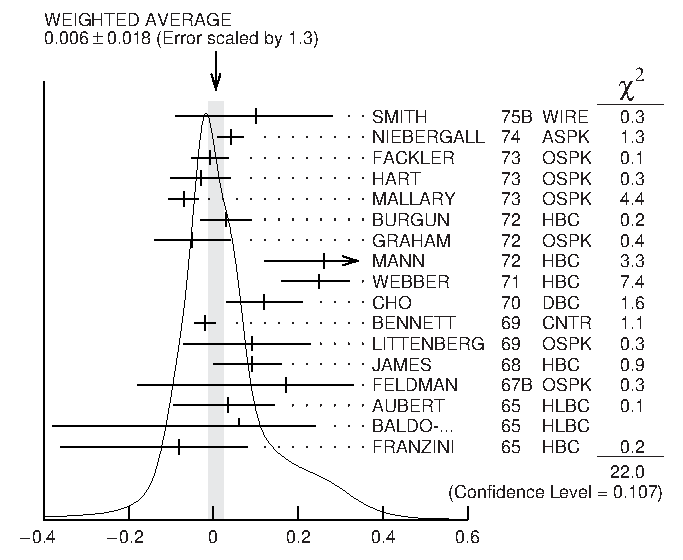
\includegraphics{filename.pdf}\hfill
	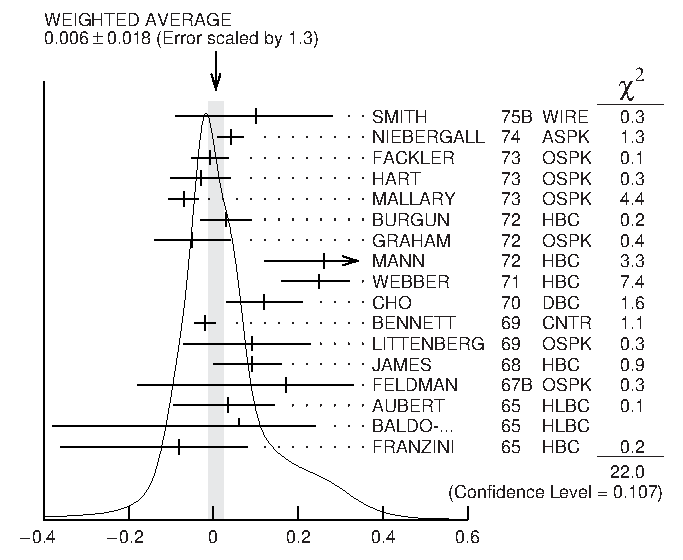
\includegraphics{filename.pdf}
	\caption{Example double wide figure, 
		with different book and web versions}
	\label{examples:fig:example2}
\end{pdgxfigure}
\end{verbtex}
\begin{pdgxfigure}[wide=true,place=h,width=0.45\textwidth] 
	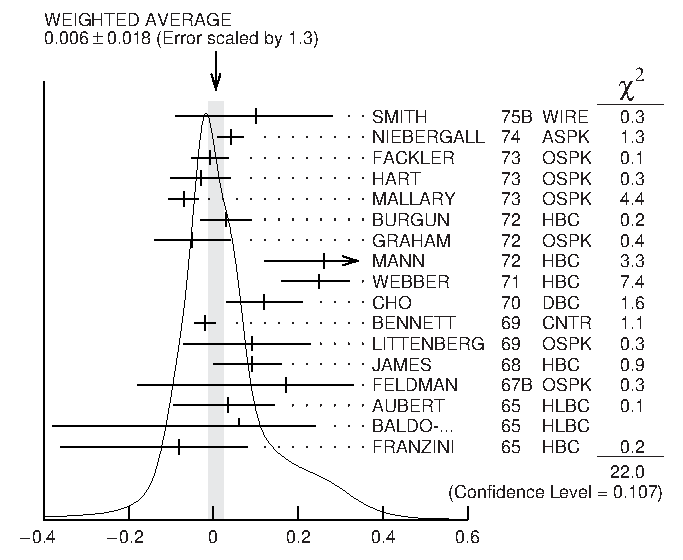
\includegraphics{filename.pdf}\hfill
	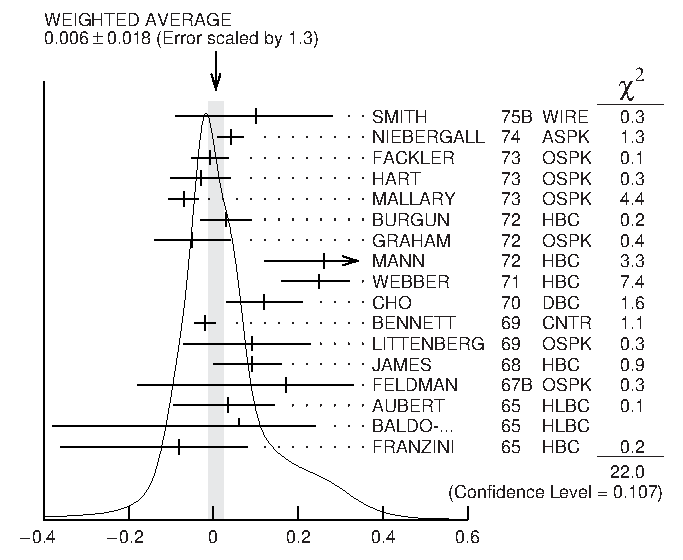
\includegraphics{filename.pdf}
	\caption{Example double wide figure, with different book and web versions}
	\label{examples:fig:example2}
\end{pdgxfigure}

A double wide figure with separate option and scaling keys, shown in Fig.~\ref{examples:fig:example3}:
\begin{verbtex}
\begin{pdgxfigure}[wide=true,place=h,width = 0.3\linewidth] 
	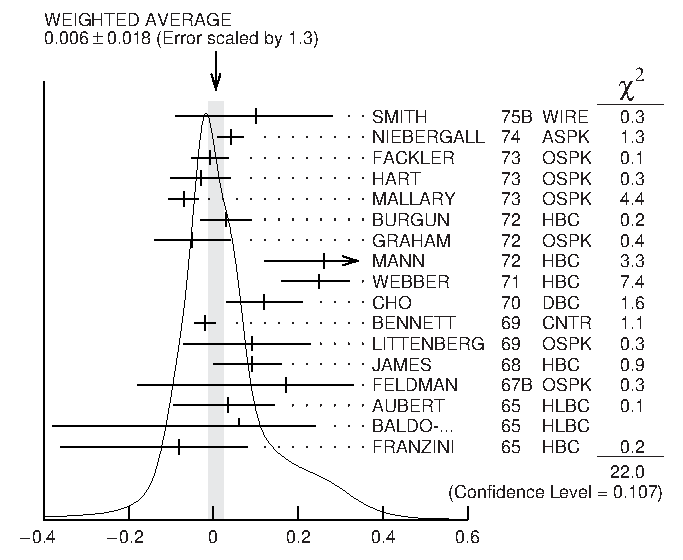
\includegraphics{filename.pdf}\hspace{1cm}
	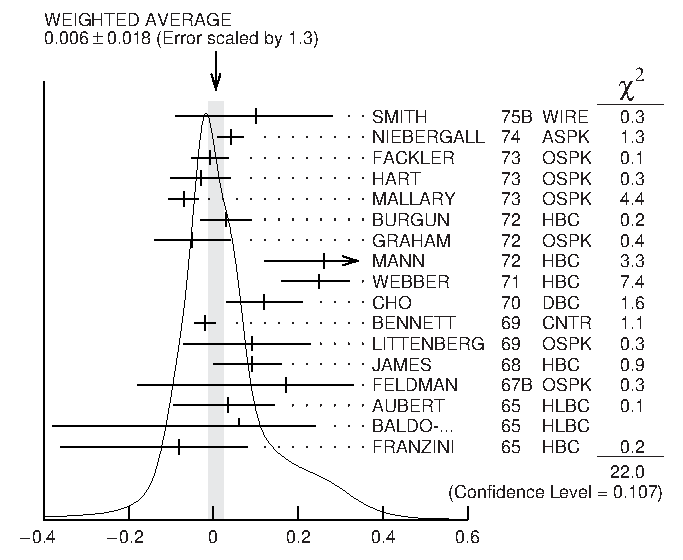
\includegraphics[width = !,scale =0.3,angle = 90]{filename}
	\caption{Example double figure, 
		with separate option and scaling keys, in both book and web versions}
	\label{examples:fig:example3}
\end{pdgxfigure}
\end{verbtex}
\begin{pdgxfigure}[wide=true,place=h,width = 0.3\linewidth] 
	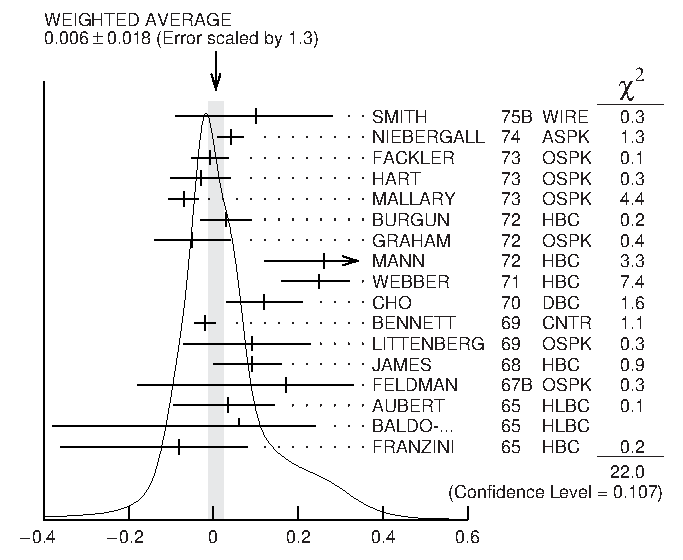
\includegraphics{filename.pdf}\hspace{1cm}
	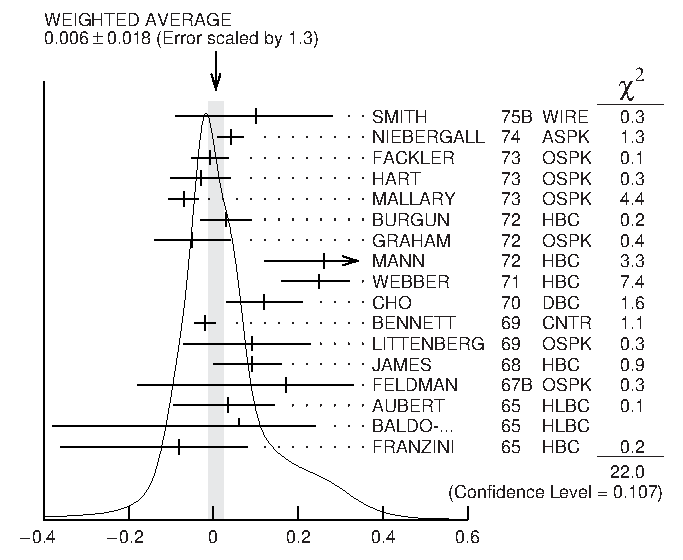
\includegraphics[width = !,scale =0.3,angle = 90]{filename}
	\caption{Example double wide figure, with separate option and scaling keys, in both book and web versions}
	\label{examples:fig:example3}
\end{pdgxfigure}

\Isubsection{\invt{pdgfigure} commands}
To add a figure, one may also use the \lstinline{\pdgfigure} or \lstinline{\pdgwidefigure} commands 
to typeset a single-column figure or double-column wide figure (for the book version), respectively. 
To include two images in one figure one may use \lstinline{\pdgdoublefigure}.
These commands are less powerful than \invt{pdgxfigure}, but automatically incorporate all PDG styles.

The macros \lstinline{\pdgfigure} and \lstinline{\pdgwidefigure} take the following arguments:
\begin{verbtex}
	\pdgfigure{<filename>}
	{<caption>}{<label>}{<placement options>}
	{<other option keys>}
\end{verbtex}
\vspace{-10pt}
while the macro \lstinline{\pdgdoublefigure} takes the following arguments:
\begin{verbtex}
	\pdgdoublefigure{<filename1>}{<filename2>}
	{<caption>}{<label>}{<placement options>}
	{<other option keys>}
\end{verbtex}
Some examples of the \invt{pdgfigure} commands are shown in Figs.~\ref{examples:fig:ideogram1}, \ref{examples:fig:ideogram2} and \ref{examples:fig:ideogram3}, respectively:
\begin{verbtex}
	\pdgfigure{filename.pdf}{Figure with caption and label}
	{examples:fig:ideogram1}{ht!}{}
	
	\pdgdoublefigure{filename.pdf}{filename.pdf}
	{Two figures, with caption and label, reduced in size}
	{examples:fig:ideogram2}{ht!}{width=0.3\textwidth}
	
	\pdgwidefigure{filename.pdf}{Wide figure}
	{examples:fig:ideogram3}{t}{}
\end{verbtex}
\FloatBarrier
\pdgfigure{filename.pdf}{Figure with caption and label}{examples:fig:ideogram1}{ht!}{}
\pdgdoublefigure{filename.pdf}{filename.pdf}{Two figures, with caption and label, reduced in size}{examples:fig:ideogram2}{ht!}{width=0.3\textwidth}
\pdgwidefigure{filename.pdf}{Wide figure}{examples:fig:ideogram3}{t}{}
\FloatBarrier

\Isection{Tables}
\label{sec:tables}
\Isubsection{ \invt{pdgxtable} and \invt{pdgxtabular}}
The PDG class provides multipurpose table and tabular environments, \invt{pdgxtable} and \invt{pdgxtabular}. 
These operate similarly to the standard \invt{table} and \invt{tabular} environments: \invt{(pdgx)table} creates a floating environment, 
while \invt{(pdgx)tabular} creates the actual tabulated display. 

The \lstinline!\caption! and \lstinline!\label! commands may be used as in the usual \invt{table} environment.
\textbf{Note: A table caption should be placed above the table.}
In addition, \invt{pdgxtable} takes a wide array of additional option keys that implement features and formatting of the prior PDG table commands/environments.  
These include keys that control placement, multicolumn spanning, version-specific widths and scaling (see Sec.~\ref{sec:ginkeys}), rotation, stretching, and caption widths.
The generic usage is
\begin{verbtex}
\begin{pdgxtable}[<option keys>]
	\caption{This is a PDG table}
	\label{tab:label}
	\begin{pdgxtabular}{<column settings>} % the usual c, l, r, | etc
		\pdgtableheader{...} %column header & separated entries go here
		%table & separated entries go here
	\end{pdgxtabular}
	%multiple pdgtabular environments are allowed
\end{pdgxtable}
\end{verbtex}

As for the usual \invt{table} environment, one may include multiple \invt{pdgxtabular}s in a single \invt{pdgxtable}.
While the \invt{pdgxtable} environment has default handling for caption widths in wide and regular tables, for both book and web versions, 
absolute control of the caption width can be implmented with a \lstinline{\captionsetup} command inside the \invt{pdgxtable} environment. 
For example \lstinline!\captionsetup{width=\linewidth}! gives a full width caption.

\Isubsection{Available keys for \invt{pdgxtable}}
Following is a list of available optional keys, and default settings if not invoked.
As usual, keys are evaluated left to right. 
While, the version-general \invt{width} key can be used (and will override any preceeding version-specfic width key), 
there is no version-general \invt{scale} key. 
Scaling of the tables is best done with the \invt{<version>scale} keys.

\begin{itemize}
	\item \invt{place}: Takes any combination of \invt{h}, \invt{t}, \invt{b}, \invt{p} (with optional \invt{\!}) that specifies float placement. Default is \invt{\!ht}.
	\item \invt{wide}: Takes \invt{true} or \invt{false} to specify the table as full page width in either single or two column mode. Default is \invt{false}.
	\item \invt{width} or \invt{<version>width}: Sets the version specific maximum width of the table bounding box. 
	Default is the maximum text width implied by the \invt{wide} key setting.
	Width settings exceeding this default are ineffective. Footnotes are scaled, but caption width is not affected.
	\item \invt{<version>scale}: Scales the table according to float value passed to the key. 
	For overwide tables, there is always a value $<1$ at which the table will be properly set to maximum page width.
	Footnotes are scaled, but caption width is not affected. Note the global \invt{scale} is disabled for \invt{pdgxtable}.
	\item \invt{<version>bbscale}: Scales the bounding box of the table. 
	For some overwide tables that are larger than the nominal page width, simply rescaling down the table does not allow the table to be properly aligned on the page.
	This key can be increased above $1$ (the default), to provide a sufficiently large bounding box for the table, that may then be scaled down to size with correct alignment.
	\item \invt{widecaptionscale}: For \invt{wide = true} tables, scales the caption width with respect to the maximum page width. Default is $0.75$.
	\item \invt{narrowcaptionscale}: For \invt{wide = false} or default tables, scales the caption width with respect to the maximum column width. Default is $0.9$.
	\item \invt{rotated}: Takes \invt{left} or \invt{right} to rotate the table, but not the caption, $90^\circ$ anticlockwise or clockwise, respectively. 
	The caption may be rotated independently, as needed with a \lstinline{\rotatebox}.
	\item \invt{sideways}: Takes \invt{true} or \invt{false} to rotate the table, including the caption, $90^\circ$ anticlockwise or clockwise, 
	according to whether the page number is even or odd.
	In a sideways table, other key width and scaling settings are still effective, but scale with respect to the page height. 
\end{itemize}


\Isubsection{Examples}
Some (simple) examples of \invt{pdgxtable} can be found in Table~\ref{examples:tab:styles} and Sec~\ref{sec:macros}.
For example, Tab.~\ref{examples:tab:styles} is typeset as
\begin{verbtex}
\begin{pdgxtable}[place=h,bookscale = 0.9,bookbbscale=2]
	\caption{Styles for the different typesetting versions}
	\label{examples:tab:styles}
	\begin{pdgxtabular}{ccccc}
		Version 		& Columns  & Font size 	& Helper Tags\footnote{
			Tags for each equation, table, figure, and bibliography entry 
			are displayed in margin or interspaced} & Line numbers\\
		\hline
		draft	& 1		   & 11pt		& Yes & Yes \\
		...
	\end{pdgxtabular}
\end{pdgxtable}
\end{verbtex}

Tables~\ref{examples:tab:commu} and~\ref{examples:tab:commp} are typeset as a two \invt{pdgxtabular}s in a single \invt{pdgxtable}, via
\begin{verbtex}
\begin{pdgxtable}[wide=true, place=!ht, webscale = 0.8]
	\caption{Common units}
	\label{examples:tab:commu}
	\begin{pdgxtabular}{lr | lr | lr}
		\showsymbol{\TeV} &  \showsymbol{\syin} & \showsymbol{\barn}   \\
		...
	\end{pdgxtabular}
	\caption{Common particles}
	\label{examples:tab:commp}
	\begin{pdgxtabular}{lr | lr | lr}
   		\showsymbol{\pp} &  \showsymbol{\ee} & \showsymbol{\pizero}   \\
  		...
	\end{pdgxtabular}
\end{pdgxtable}
\end{verbtex}

\Isubsection{Common problems and recommendations}
The \invt{pdgxtabular} environment is capable of handling the usual \lstinline{\multicolumn} and \lstinline{\multirow} objects, 
that allow for more complicated tables with cells spanning multiple rows and/or columns. 
We recommend avoiding use of \lstinline{\multispan}. 
For multiline cells, the \lstinline{\makecell} command from the \invt{makecell} package is recommended.

\Isection{Labels and referencing}
\label{sec:labels}

\Isubsection{Style guide}
As usual, the \lstinline{\label} and \lstinline{\ref} commands (and their derivatives) may be used to reference equations, tables, figures, and so on. 
To permit easy cross-referencing throughout the entire review, we request that you use the following labelling convention: \invt{BASENAME:type:name}
with \invt{type} corresponding to one of the following options
\begin{itemize}
\item {\tt fig} for figures
\item {\tt eq } for equation
\item {\tt tab} for tables
\item {\tt sec} for section, subsection etc..
\item {\tt foot} for footnotes.
\end{itemize}

\Isubsection{Missing references}

In default LaTeX, missing references are typically typeset as ``\textbf{??}''. 
To improve the typesetting experience, the \lstinline{\ref} command has been modified in the PDG class so that missing reference keys are printed out explicitly: 
For instance, a \lstinline!\ref{eqn:name}! that references a missing label called \invt{eqn:name}, will display as \ref{eqn:name}.
Similarly, the \lstinline{\cite} command will explicitly print out missing citation references. E.g. 
a \lstinline!\cite{name:2021ab}! that references a missing label called \invt{name:2021ab}, will display as \cite{name:2021ab}

\Isubsection{Cross-review referencing}
It is occasionally necessary or useful to reference (sub)sections, equations, figures, tables and so on belonging to other reviews or other reviews themselves. 
\textbf{Note:} Please use the \lstinline{\crossref} command for cross-review referencing.

Implementing a cross-reference to another review requires knowledge of its  \invt{BASENAME}:  
You must use the \invt{BASENAME} associated with the target review, not the \invt{BASENAME} of the review you're currently working on. 
To identify the  \invt{BASENAME} of another review, login into the \href{https://pdgworkspace.lbl.gov/Reviews.action}{PDG Workspace} (click to be redirected). 
Under \emph{Reviews} select from the drop-down menu \emph{All reviews}. 
Click on the title of the review you are interested in, and then select the \emph{Technical details} tab. 
The \invt{BASENAME} is the first entry.


If the full \invt{BASENAME:type:name} reference is known, you may include it with the usage \\
\lstinline!\crossref{BASENAME:type:name}!. 
This will typeset in your document as ``\crossref{BASENAME:type:name}'', because your local auxiliary files do not have the reference information of the other review.
PDG editorial staff will implement the cross-reference properly, when your review is prepared for production.

If the \invt{BASENAME:type:name} reference is not known, or the authors of the other review did not label the obect that you wish to reference, 
you may instead provide any descriptive argument to \lstinline{\crossref}. 
For example, \lstinline!\crossref{Equation 34.1.10}!.  
PDG editorial staff will implement the cross-reference properly, when your review and the other review are prepared for production.

\Isubsection{Booklet labeling and referencing}
If your review has a booklet version, it needs to be prepared at the same time as you prepare your full review.
The content to be displayed in the booklet needs to be included in \invt{BASENAME-booklet.tex}. 

The numerical tags for equations, tables, and figures in the booklet version of a review should match the tags in the full version. 
This can be achieved automatically in the booklet version by using a \lstinline!\tag{\ref{BASENAME:type:name}}! construction instead of \lstinline{\label}
to refer to the reference in the full version.
For example, if the full version has a labelled equation
\begin{verbtex}
\begin{equation}
	\label{BASENAME:eq:name}
	...
\end{equation}
\end{verbtex}
then including in \invt{BASENAME-booklet.tex}
\begin{verbtex}
\begin{equation}
	\tag{\ref{BASENAME:eq:name}}
	...
\end{equation}
\end{verbtex}
will automatically label the equation correctly. 
To achieve the same result for figures and tables, one may place in the booklet version
\begin{verbtex}
	\renewcommand{\thetable}{\ref{BASENAME:type:name}}
	\renewcommand{\thefigure}{\ref{BASENAME:type:name}}
\end{verbtex}
before each table or figure environment, respectively. 


\Isection{Index entries}
\label{sec:index}

Review authors should think about any keywords that should be included into the index of the Review of Particle Physics. PDG uses the standard \LaTeX\  \invt{makeidx} package. Thus an entry ``sample text'' can be added to the index by placing
\begin{verbtex}
\index{sample text}
\end{verbtex}
at the appropriate place in the source file. Formatting of entries with Greek letters or math symbols as well as subentries are also supported. For example
\begin{verbtex}
\index{sigma@$\$$\sigma$\$$} 
\end{verbtex}
creates an index entry $\sigma$ in the proper alphabetical order, while
\begin{verbtex}
\index{Searches!Axion searches} 
\end{verbtex}
produces a subentry ``Axion searches'' under the ``Searches'' index entry.

All index entries defined in a given review will be shown on the last page when the draft version is made. PDG staff will standardize all index entries during the final processing of all reviews. Therefore what matters is not the final formatting of index entries but that all relevant entries are added in the correct place.


\Isection{Bibliography}
\label{sec:cites}

Citations are handled using BibTeX. To add a citation to your review:
\begin{itemize}
\item Look up the reference in INSPIRE and download its BibTeX entry (see bottom of the \emph{Information} tab for the article, under \emph{Export}).
\item Add the BibTeX entry to the \invt{BASENAME.bib} file. Note the article tag assigned by INSPIRE: You can see it in the first line of the BibTeX entry, after \lstinline!@article{!.
\item Cite the reference with \lstinline{\cite}, using the article tag assigned by INSPIRE.
\end{itemize}

For example, to add a reference to the Review of Particle Physics (2018) 
add the following code to \invt{BASENAME.bib}:
\begin{verbtex}
@article{Tanabashi:2018oca,
      author         = "Tanabashi, M. and others",
      title          = "{Review of Particle Physics}",
      collaboration  = "Particle Data Group",
      journal        = "Phys. Rev.",
      volume         = "D98",
      year           = "2018",
      number         = "3",
      pages          = "030001",
      doi            = "10.1103/PhysRevD.98.030001",
      SLACcitation   = "%%CITATION = PHRVA,D98,030001;%%"
 }
\end{verbtex}
and then one may add a reference to it in \invt{BASENAME-main.tex} via \lstinline!\cite{Tanabashi:2018oca}!.

If a BibTeX entry downloaded from INSPIRE does not render correctly, 
you should first make sure you have the latest PDG style files, by running \invt{svn update} (after committing any edits you have made).
If this doesn't fix the issue please contact \invt{latexsupport@pdg.lbl.gov} for advice.  
If it appears, however, to be simply a mistake in INSPIRE's entry, 
rename the label to the form \invt{BASENAME:<INSPIRE label>} and then edit the entry as needed.
\textbf{Please do not edit entries downloaded from INSPIRE without changing the label.}
Changing the label will permit PDG editorial staff to easily identify and track edited citations, as well as notify INSPIRE of required corrections.
In case the reference does not appear in INSPIRE at all, please also use the convention for the label: \invt{BASENAME:name}.

Multiple references can be added to a single set of brackets with \lstinline!\cite{cite-key-1,cite-key-2,...}!.
One may group multiple references into the same numerical citation tag, using a \invt{*} prefix on subsequent citation keys: For example \lstinline!\cite{cite-key-1,*cite-key-2,*cite-key-3}!.
If a paper citation key is preceded by the asterisk, it can't be cited separately later, and doing so will result in a compilation error.
We recommend citing papers individually, without using the asterisk to group them.


\Isection{Footnotes}
Footnote styles are standardized throughout the review. In (rare) cases that the style needs to be changed, this is achieved via \lstinline!\setfootnotestyle{<style>}!,
where \invt{<style>} can be \lstinline{\fnsymbol} or \lstinline{\alph}, \lstinline{\Alph}, \lstinline{\arabic}, \lstinline{\roman}, \lstinline{\Roman} etc.

Sometimes the \LaTeX \ engine miscalculates the amount of space required for a footnote, resulting in overprinting of the footer.
One can help the engine obtain a better estimate by adjusting the effective page size. 
This can be done by placing \lstinline!\enlargethispage{-2\baselineskip}! somewhere just before the \lstinline{\footnote}; the \invt{-2} may be changed to any number. 

\Isection{Miscellaneous control commands}

\Isubsection{Unbalanced last page}
In the book version, the columns of the final page are automatically balanced. 
If this behavior is undesired, it may be altered by invoking \lstinline!\balancedlastpagefalse!.
The invocation may be added anywhere in the document.

\Isubsection{Blank last page}
In the book version, a blank final page may be added via \lstinline!\blankendpagetrue!.
The invocation may be added anywhere in the document.

\Isubsection{Book-only reviews}
Certain reviews are typeset for the web using the book version formatting. 
This is enforced automatically within the PDG system by \lstinline!\def\iswebbook{1}! before the \lstinline{\documentclass} invocation. 
The draft version, however, for such reviews are typeset in the usual draft/web format.

\clearpage
\Isection{PDG Macros}
\label{sec:macros}

\begin{pdgxtable}[wide=true, place=!ht, webscale = 0.8]
	\vspace{-10pt}
	\caption{Common units}
	\label{examples:tab:commu}
	\begin{pdgxtabular}{lr | lr | lr}
		\showsymbol{\TeV     } &  \showsymbol{\syin} & \showsymbol{\barn     }   \\
		\showsymbol{\MeV     } &  \showsymbol{\inch} & \showsymbol{\mbarn    }   \\
		\showsymbol{\keV     } &  \showsymbol{\ft  } & \showsymbol{\microbarn}   \\
		\showsymbol{\eV      } &  \showsymbol{\km  } & \showsymbol{\nb       }   \\
		\showsymbol{\GeVc    } &  \showsymbol{\m   } & \showsymbol{\pb       }   \\
		\showsymbol{\GeVcSq  } &  \showsymbol{\cm  } & \showsymbol{\fb       }   \\
		\showsymbol{\GeVcc   } &  \showsymbol{\mm  } & \showsymbol{\invnb    }   \\
		\showsymbol{\GeVccSq } &  \showsymbol{\mum } & \showsymbol{\invpb    }   \\
		\showsymbol{\MeVc    } &  \showsymbol{\nm  } & \showsymbol{\invfb    }   \\
		\showsymbol{\MeVcc   } &  \showsymbol{\fm  } & \showsymbol{\invab    }   \\
		\showsymbol{\invps   } &  \showsymbol{\nm  } & \showsymbol{\lum      }   \\
			&&  \showsymbol{\ma  } &&  \\
		\showsymbol{\degr    }  &  \showsymbol{\cma } && \\
			&&  \showsymbol{\mma } &&   \\
			&&  \showsymbol{\muma} &&   \\
	\end{pdgxtabular}
	\vspace{10pt}
	\caption{Common particles}
	\label{examples:tab:commp}
	\vspace{-10pt}
	\begin{pdgxtabular}{lr | lr | lr}
   \showsymbol{\pp         } &  \showsymbol{\ee           } & \showsymbol{\pizero   }   \\
   \showsymbol{\pbar       } &  \showsymbol{\epm          } & \showsymbol{\piplus   }   \\
   \showsymbol{\ppbar      } &  \showsymbol{\epem         } & \showsymbol{\piminus  }   \\
   \showsymbol{\tbar       } &  \showsymbol{\en           } & \showsymbol{\pipm     }   \\
   \showsymbol{\ttbar      } &  \showsymbol{\ep           } & \showsymbol{\pimp     }   \\
   \showsymbol{\bbar       } &  \showsymbol{\mumu         } & \showsymbol{\etaprime }   \\
   \showsymbol{\bbbar      } &  \showsymbol{\mun          } & \showsymbol{\Kzero    }   \\
   \showsymbol{\cbar       } &  \showsymbol{\mup          } & \showsymbol{\Kzerobar }   \\
   \showsymbol{\ccbar      } &  \showsymbol{\tautau       } & \showsymbol{\kaon     }   \\
   \showsymbol{\sbar       } &  \showsymbol{\taup         } & \showsymbol{\Kplus    }   \\
   \showsymbol{\ssbar      } &  \showsymbol{\taum         } & \showsymbol{\Kminus   }   \\
   \showsymbol{\ubar       } &  \showsymbol{\lepton       } & \showsymbol{\KzeroL   }   \\
   \showsymbol{\uubar      } &  \showsymbol{\leptonm      } & \showsymbol{\Kzerol   }   \\
   \showsymbol{\dbar       } &  \showsymbol{\ellm         } & \showsymbol{\Klong    }   \\
   \showsymbol{\ddbar      } &  \showsymbol{\leptonp      } & \showsymbol{\KzeroS   }   \\
   \showsymbol{\fbar       } &  \showsymbol{\ellp         } & \showsymbol{\Kzeros   }   \\
   \showsymbol{\ffbar      } &  \showsymbol{\leptonlepton } & \showsymbol{\Kshort   }   \\
   \showsymbol{\qbar       } &  \showsymbol{\ellell       } & \showsymbol{\Kstar    }   \\
   \showsymbol{\qqbar      } &  \showsymbol{\enu          } & \showsymbol{\jpsi     }   \\
   \showsymbol{\nbar       } &  \showsymbol{\munu         } & \showsymbol{\Jpsi     }   \\
   \showsymbol{\nnbar      } &  \showsymbol{\taunu        } & \showsymbol{\psip     }   \\
   \showsymbol{\neutron    } &  \showsymbol{\lnu          } & \showsymbol{\chic     }   \\
   \showsymbol{\antineutron} &  \showsymbol{\nub          } & \showsymbol{\UoneS    }   \\
   \showsymbol{\deuteron   } &  \showsymbol{\nunub        } & \showsymbol{\chib     }   \\
   \showsymbol{\Zzero      } &  \showsymbol{\nue          } & \showsymbol{\Dstar    }   \\
   \showsymbol{\Zboson     } &  \showsymbol{\nueb         } & \showsymbol{\Bd       }   \\
   \showsymbol{\Wplus      } &  \showsymbol{\nuenueb      } & \showsymbol{\Bs       }   \\
   \showsymbol{\Wminus	   } &  \showsymbol{\num          } & \showsymbol{\Bu       }   \\
   \showsymbol{\Wboson	   } &  \showsymbol{\numb         } & \showsymbol{\Bc       }   \\ 
   \showsymbol{\Wpm   	   } &  \showsymbol{\numnumb      } & \showsymbol{\Lb       }   \\
   \showsymbol{\Wmp        } &  \showsymbol{\nut          } & \showsymbol{\Bstar    }   \\
   \showsymbol{\Hzero } &  \showsymbol{\nutb         } & \showsymbol{\BoBo     }   \\
   \showsymbol{\Hboson}  &	\showsymbol{\nutnutb      } & \showsymbol{\BodBod   }    \\		    
   \showsymbol{            } &	\showsymbol{              } & \showsymbol{\BosBos   }    \\		    
   \showsymbol{            } &	\showsymbol{              } & \showsymbol{\LambdaStar}  \\
	\end{pdgxtabular}
\end{pdgxtable}

\begin{pdgxtable}[wide=true, place=h, webscale = 0.8]
	\caption{Hypothetical particles}
	\begin{pdgxtabular}{lr | lr | lr}
   \showsymbol{\Azero }      &  \showsymbol{\gravino   } & \showsymbol{\slepton   }   \\
   \showsymbol{\hzero }      &  \showsymbol{\Zprime    } & \showsymbol{\sleptonL  }   \\
   \showsymbol{\Hzero }      &  \showsymbol{\Zstar     } & \showsymbol{\sleptonR  }   \\
   \showsymbol{\Hplus }  	  &  \showsymbol{\squark    } & \showsymbol{\sel       }   \\
   \showsymbol{\Hminus}       &  \showsymbol{\squarkL   } & \showsymbol{\selL      }   \\
   \showsymbol{\Hpm   }   	&  \showsymbol{\squarkR   } & \showsymbol{\selR      }   \\
   \showsymbol{\Hmp   }       &  \showsymbol{\gluino    } & \showsymbol{\smu       }   \\
   \showsymbol{\ggino }     &  \showsymbol{\stop      } & \showsymbol{\smuL      }   \\
   \showsymbol{\chinop}      &  \showsymbol{\stopone   } & \showsymbol{\smuR      }   \\
   \showsymbol{\chinom}      &  \showsymbol{\stoptwo   } & \showsymbol{\stau      }   \\
   \showsymbol{\chinopm}      &  \showsymbol{\stopL     } & \showsymbol{\stauL     }   \\
   \showsymbol{\chinomp}     &  \showsymbol{\stopR     } & \showsymbol{\stauR     }   \\
   \showsymbol{\chinoonep}     &  \showsymbol{\sbottom   } & \showsymbol{\stauone   }   \\
   \showsymbol{\chinoonem}   &  \showsymbol{\sbottomone} & \showsymbol{\stautwo   }   \\
   \showsymbol{\chinoonepm}   &  \showsymbol{\sbottomtwo} & \showsymbol{\snu       }   \\
   \showsymbol{\chinotwop}  &  \showsymbol{\sbottomL  } & \showsymbol{           }   \\
   \showsymbol{\chinotwom}   &  \showsymbol{\sbottomR  } & \showsymbol{           }   \\
   \showsymbol{\chinotwopm}   &  \showsymbol{           } & \showsymbol{           }   \\
   \showsymbol{\nino}  &  \showsymbol{           } & \showsymbol{           }   \\
   \showsymbol{\ninoone}        &  \showsymbol{           } & \showsymbol{           }   \\
   \showsymbol{\ninotwo}     &  \showsymbol{           } & \showsymbol{           }   \\
   \showsymbol{\ninothree}     &  \showsymbol{           } & \showsymbol{           }   \\
   \showsymbol{\ninofour}   &  \showsymbol{           } & \showsymbol{           }   \\
	\end{pdgxtabular}
\vspace*{10pt}
	\caption{Useful symbols for proton-proton physics}
\vspace*{-10pt}	
	\begin{pdgxtabular}{lr | lr }
   \showsymbol{\pT  }      &  \showsymbol{\rts }   \\
   \showsymbol{\pt  }      &  \showsymbol{\sqs } \\
   \showsymbol{\ET  }      &  \showsymbol{\mh}  \\
   \showsymbol{\eT  }      &  \showsymbol{\mW}  \\
   \showsymbol{\et  }      & \showsymbol{\mZ}   \\
   \showsymbol{\HT  }      & \showsymbol{\mH}   \\
   \showsymbol{\pTsq}      &&   \\
   \showsymbol{\MET }      &&   \\
   \showsymbol{\met }      &&   \\
   \showsymbol{\Ecm }      &&   \\
	\end{pdgxtabular}
\vspace*{10pt}
	\caption{Monte Carlo Generators}
\vspace*{-10pt}		
	\begin{pdgxtabular}{lr | lr | lr}	
   \showsymbol{\ACERMC    }      &  \showsymbol{\MCatNLO   } & \showsymbol{\Comphep    }   \\
   \showsymbol{\ALPGEN    }      &  \showsymbol{\AMCatNLO  } & \showsymbol{\Prospino   }   \\
   \showsymbol{\GEANT     }      &  \showsymbol{\MCFM      } & \showsymbol{\LO         }   \\
   \showsymbol{\Herwigpp  }      &  \showsymbol{\METOP     } & \showsymbol{\NLO        }   \\
   \showsymbol{\HERWIGpp  }      &  \showsymbol{\POWHEG    } & \showsymbol{\NLL        }   \\
   \showsymbol{\Herwig    }      &  \showsymbol{\POWHEGBOX } & \showsymbol{\NNLO       }   \\
   \showsymbol{\HERWIG    }      &  \showsymbol{\POWPYTHIA } & \showsymbol{\muF        }   \\
   \showsymbol{\JIMMY     }      &  \showsymbol{\PROTOS    } & \showsymbol{\muR        }   \\
   \showsymbol{\MADSPIN   }      &  \showsymbol{\PYTHIA    } & \showsymbol{            }   \\
   \showsymbol{\MADGRAPH  }      &  \showsymbol{\SHERPA    } & \showsymbol{            }   \\
   \showsymbol{\MGMCatNLO }      &  \showsymbol{           } & \showsymbol{            }   \\
	\end{pdgxtabular}
\end{pdgxtable}

\Isection{Tables: Legacy commands}

Though no longer recommended, legacy \lstinline{\pdgtable} or \lstinline{\pdgwidetable} commands 
to typeset a single-column table or double-column wide table (for the book version), respectively.
The \lstinline{\pdgtableheader} macro may be used in the first line of the table to automatically typeset a header.

The macros \lstinline{\pdgtable} and \lstinline{\pdgwidetable} take the following arguments:
\begin{verbtex}
	\pdgtable{<column styles>}
	{<caption>}{<label>}{<option keys>}
\end{verbtex}
Some examples usages of these commands follow, in Tables~\ref{examples:tab:table1}, \ref{examples:tab:table2} and~\ref{examples:tab:table3} below.
\begin{verbtex}
\begin{pdgtable}{c c c} 
	{Table}{examples:tab:table1}{h!}
	\pdgtableheader{ Column 1 & Column 2 & Column 3}
	row1  & 1  & 2\\
	row2  & 1  & 2\\
	row3  & 1  & 2\\
\end{pdgtable}
\end{verbtex}   
\begin{verbtex}
\begin{pdgtable}{|c | c | c | c|} 
	{Multicolumn table}{examples:tab:table2}{h!}
	\pdgtableheader{ \multicolumn{2}{c}{Column 1} & 
	\multicolumn{2}{c}{Column 2}}
	\pdgtableheader{ A & B& C & D }
	row1  & 1 & 2 &3 \\
	row2  & 1 & 2 &3 \\
\end{pdgtable}
\end{verbtex}  
\begin{verbtex}
\begin{pdgtable}{c l}
	{Table with footnotes}{examples:tab:table3}{}
	One value & another\footnote{This is something to notice
	\label{kmmix:foot:one}}\\
	Two values\footref{kmmix:foot:one} & another \\
\end{pdgtable}
\end{verbtex} 
 
\FloatBarrier 
\begin{pdgtable}{c c c} 
{Table}{examples:tab:table1}{h!}
\pdgtableheader{ Column 1 & Column 2 & Column 3}
row1  & 1  & 2\\
row2  & 1  & 2\\
row3  & 1  & 2\\
\end{pdgtable}
\begin{pdgtable}{|c | c | c | c|} 
{Multicolumn table}{examples:tab:table2}{h!}
\pdgtableheader{ \multicolumn{2}{|c|}{Column 1} & 
\multicolumn{2}{|c|}{Column 2}}
\pdgtableheader{ A & B& C & D }
row1  & 1 & 2 &3 \\
row2  & 1 & 2 &3 \\
\end{pdgtable}
\begin{pdgtable}{c l}
{Table with footnotes}{examples:tab:table3}{}
One value & another\footnote{This is something to notice\label{kmmix:foot:one}}\\
Two values\footref{kmmix:foot:one} & another \\
\end{pdgtable}
